\chapter{Introduction}
\label{chap:introFR}

\section{Introduction en fran\c cais}

\subsection{Analyse de donn\'ee et apprentissage automatique}

%\paragraph*{Data Analysis and Machine Learning.} 

La g\'en\'eration et l'accumulation de donn\'ees dans des secteurs d'activit\'es vari\'es, autant industriels qu'acad\'emiques,
ont pris beaucoup d'importance au cours des derni\`eres ann\'ees, et 
sont maintenant omnipr\'esents dans de nombreux domaines scientifiques, financiers et industriels.
A titre d'exemple, en science du num\'erique, le d\'eveloppement rapide des processus d'acquisition et de traitement d'images ont permis
la mise \`a disposition publique en ligne d'importantes bases de donn\'ees~\cite{Lecun98, Krizhevsky09, Nene96, Ojala02, Russell08}.
De la m\^eme mani\`ere, en biologie, la nouvelle g\'en\'eration de s\'equenceurs ont permis \`a la plupart des laboratoires d'ais\'ement d\'eterminer
%avoir acc\`es \`a 
l'ADN de diff\'erents organismes~\cite{Bindewald06,Goodwin16,Kim16,Metzker10}. 
Ainsi, la synth\'etisation et l'extraction d'informations utiles \`a partir de ces bases de donn\'ees massives sont devenus des probl\`emes d'int\'er\^et majeur.

%Data collection and generation in different human activities, including both industry and academia, have grown 
%exponentially over the last decade and are now ubiquitous in many different fields of science, finance and industry.
%For example, in digital science, the fast development of image acquisition and processing has allowed large amounts of images to 
%become publicly available online~\cite{Lecun98, Krizhevsky09, Nene96, Ojala02, Russell08}.
%Similarly, in biology, next generation high-throughput sequencing allowed most laboratories 
%to easily determine DNA sequences of sample organisms~\cite{Bindewald06,Goodwin16,Kim16,Metzker10}.  
%Hence, the summarization and the extraction of useful information from these massive amounts of data has become a problem of primary interest.

L'apprentissage automatique est un domaine de la science des donn\'ees dont le but est de fournir des algorithmes ("automatique") pouvant r\'ealiser des
pr\'edictions sur de nouvelles donn\'ees \`a partir seulement de  l'information d\'ej\`a pr\'esente dans des donn\'ees pr\'ealablement collect\'ees ("apprentissage").
Ces techniques permettent de r\'epondre \`a de multiples probl\`emes de l'analyse de donn\'ees, tels que la {\em classification}, o\`u l'on cherche
\`a pr\'edire des labels, le {\em clustering}, o\`u l'on cherche \`a regrouper les donn\'ees en diff\'erents groupes, ou la {\em r\'egression}, o\`u l'on
cherche \`a approcher une fonction \`a partir de sa valeur sur les points de donn\'ees. Nous orientons le lecteur d\'esireux de trouver plus de d\'etails
vers~\cite{Friedman01} pour une introduction compl\`ete de ces probl\'ematiques.
Par exemple, un probl\`eme typique de classification est la pr\'ediction de la pr\'esence ou non d'effets d'un m\'edicament sur un patient $P$. Il s'agit 
d'un probl\`eme de classification binaire en cela que les labels \`a pr\'edire sont au nombre de deux, \`a savoir "effet" ou "sans effet".
En supposant qu'une base de donn\'ees est disponible, dans laquelle sont enregistr\'es les effets ou non du m\'edicament sur plusieurs patients, 
une des mani\`eres les plus simples de proc\'eder est de chercher le patient le plus proche de $P$ dans la base de donn\'ees, et d'attribuer
\`a $P$ le label de ce patient. Cette m\'ethode, simple quoique tr\`es efficace, s'appelle la pr\'ediction par le plus proche voisin,
et a d\'ej\`a \'et\'e \'etudi\'ee en d\'etail. Plus g\'en\'eralement, la pr\'ediction par le plus proche voisin n'est qu'une m\'ethode parmi de nombreuses autres
en apprentissage automatique, qui peuvent traiter de probl\`emes aussi vari\'es que la classification d'images, la pr\'ediction du genre musical
ou le diagnostic m\'edical, pour ne citer que quelques exemples.
D'autres exemples d'applications sont pr\'esent\'es dans~\cite{Friedman01}. %\`a l'adresse \url{https://en.wikipedia.org/wiki/List_of_datasets_for_machine_learning_research}}.
 



%Machine Learning is a field of data science that aims at deriving algorithms ("Machine") that can 
%predict new data solely from the information that is contained in already collected datasets ("Learning").
%These techniques provide answers to multiple data analysis problems such as {\em classification}, which aims at predicting labels,
%{\em clustering}, which aims at separating data into groups or clusters, or {\em regression}, which aims at approximating functions on data.
%We refer the interested reader to~\cite{Friedman01} for a comprehensive introduction to these methods.
%For example, a typical classification problem would be to predict if a drug will have effects on a specific patient $P$. This is a binary classification
%problem since the label we want to predict for $P$ is either "effect" or "no effects".
%Assuming you have a database of patients at hand, in which the drug effects on each patient were recorded, one of the simplest way to proceed is
%to look for the closest match, or most similar patient, to $P$ in this database, 
%and to take the label of this match.  
%This extremely simple yet powerful method
%is called {\em nearest neighbor} prediction, and has been extensively studied by data scientists. 
%More generally, nearest neighbor prediction is nothing but a small part of the large variety of methods proposed in Machine Learning, 
%which can tackle many real-life challenges including image classification, musical genre prediction or medical prognosis to name a few\footnote{
%Examples of applications and datasets can be found on \url{https://en.wikipedia.org/wiki/List_of_datasets_for_machine_learning_research}}.
    

\paragraph*{Descripteurs.} En g\'en\'eral, les donn\'ees prennent la forme de nuage de points dans $\R^D$, o\`u $D\in\N^*$.
Chaque point de donn\'ee repr\'esente une {\em observation}, et chaque dimension, ou coordonn\'ee, repr\'esente une {\em mesure}.
Par exemple, les observations peuvent \^etre des patients, des images ou des s\'equences d'ADN, dont les mesures correspondantes seraient
des caract\'eristiques physiques (la taille, le poids, l'\^age...), le niveau de gris des pixels, ou des bases azot\'ees A, C, T ou G composant l'ADN.
Tr\`es souvent, le nombre de mesures est \'elev\'e, fournissant ainsi beaucoup d'informations, mais rendant 
dans le m\^eme temps les donn\'ees impossibles \`a visualiser.

Ainsi, une grande partie de l'analyse de donn\'ees se consacre \`a la synth\'etisation de l'information contenue dans les donn\'ees
en des {\em descripteurs} simples et interpr\'etables, qui d\'ependent en g\'en\'eral de l'application.
Par exemple, on peut touver, parmi les descripteurs usuels :
le mod\`ele sac-de-mots~\cite{Soumya14} pour les donn\'ees textuelles,
les descripteurs SIFT~\cite{Lowe04} et HoG~\cite{Dalal05} pour les images,
la courbure et les images de spin~\cite{Johnson99} pour les formes 3D,
les descripteurs en ondelettes~\cite{Mallat08} pour le traitement du signal,
et, plus g\'en\'eralement, le r\'esultat d'une technique de r\'eduction de dimension, comme l'ACP, MDS ou Isomap~\cite{Tenenbaum00}.
L'efficacit\'e des descripteurs est souvent corr\'el\'ee aux propri\'et\'es dont ils b\'en\'eficient. En fonction de l'application,
il peut \^etre pertinent d'exiger d'un descripteur qu'il soit invariant par translation ou rotation, intrins\`eque ou extrins\`eque, un vecteur Euclidien, etc.
Trouver des descripteurs avec de telles propri\'et\'es est une question importante car permettant d'am\'eliorer grandement l'interpr\'etation et la visualisation
des donn\'ees, comme mentionn\'e plus haut, mais aussi le r\'esultat des algorithmes d'apprentissage, qui sont susceptibles 
de produire de mauvaises performances si aliment\'es avec des donn\'ees brutes.
Le but de cette th\`ese est d'\'etudier une classe sp\'ecifique de descripteurs appel\'es {\em topologiques}, et qui sont connus
pour \^etre invariants aux d\'eformations continues des donn\'ees qui n'impliquent pas de d\'echirement ou de recollement~\cite{Carlsson09a}. 

%\paragraph*{Descriptors.} Usually, data comes in the form of a point cloud in $\R^D$, where $D\in\N^*$. 
%Each data point represents an {\em observation} and each dimension, 
%or coordinate, represents a {\em measurement}. For instance, observations can be patients, images or DNA sequences, whose corresponding measurements are
%physical characteristics (height, weight, age...), grey scale values of pixels or nucleobases A, C, T or G composing DNA.
%It is often the case that the number of measurements is very large, leading to a rich level of information, but also making 
%data very high-dimensional and impossible to visualize.  

%Hence, a large part of data analysis is devoted to the summarization 
%of the information contained in datasets or data points into simple and 
%interpretable {\em descriptors}, which are usually application specific. 
%For instance, among common descriptors are: 
%bag-of-words models~\cite{Soumya14} for text document data,
%SIFT~\cite{Lowe04} and HoG~\cite{Dalal05} descriptors for image data,
%curvature and spin images~\cite{Johnson99} for 3D shape data,
%wavelet descriptors~\cite{Mallat08} for signal data,
%and, more generally, outputs of any data reduction techniques, such as MDS, PCA or Isomap~\cite{Tenenbaum00}.
%The efficiency of descriptors is very often correlated to the properties they enjoy. Depending on the application,
%one may want descriptors  to be translation or rotation invariant, intrinsic or extrinsic, to lie in Euclidean space...
%Deriving descriptors with desireable properties is important since it greatly enhances interpretation and visualization, as mentioned above,
%but also the performance of Machine Learning algorithms, which may perform poorly if feeded with raw data.
%The aim of this thesis is to study a specific class of descriptors called {\em topological} descriptors, which are known to be 
%{\em stable}, in the sense that descriptors of similar data cannot be far from each other, and 
%invariant to continuous deformation of data~\cite{Carlsson09a}. Topological descriptors have been proved
%useful and helped improve data analysis in many different applications, ranging from 3D shape analysis~\cite{Carriere15a, Chazal09c} 
%to medical diagnosis~\cite{Lum13,Nicolau11,Rucco15} to
%glass material transition~\cite{Gameiro16, Hiraoka16} to genomics~\cite{Camara16,Chan13} among many others. 
  
\subsection{Descripteurs topologiques}

L'id\'ee derri\`ere les descripteurs topologiques est de synth\'etiser {\em l'information topologique} pr\'esente dans les donn\'ees~\cite{Carlsson09a}.
Intuitivement, la topologie des donn\'ees englobe toutes les propri\'et\'es qui sont pr\'eserv\'ees par des d\'eformations continues, 
comme l'\'etirement, le r\'etr\'ecissement ou l'\'epaississement, sans d\'echirure ni recollement. Par exemple, 
%l'int\'erieur d'un cercle, qui est un trou de dimension 1, est de nature topologique : 
si un cercle est continument d\'eform\'e sans d\'echirement ou recollement, un trou va toujours subsister
dans l'objet r\'esultant, quelle qu'ait \'et\'e la transformation. C'est ce qu'on appelle un {\em attribut topologique}. 
Voir la Figure~\ref{fig:deformation}, o\`u la pr\'esence d'un trou est attest\'ee dans diff\'erentes d\'eformations du cercle.

%\section{Topological Descriptors}

%The idea of topological descriptors is to summarize the {\em topological information} contained in data~\cite{Carlsson09a}.
%Intuitively, the topology of data encompasses all of its properties that are preserved under continuous deformations, such as stretching, shrinking
%or thickening without tearing or gluing. For instance, the inside of a circle, which is a 1-dimensional hole, is of topological nature: 
%if a circle is continuously deformed, a hole will always remain in the resulting object, whatever the transformation was. See Figure~\ref{fig:deform},
%where a 1-dimensional hole is always present in the displayed deformations of the circle.

\begin{figure}
\centering
\begin{minipage}{.7\textwidth}
  \centering
  
\includegraphics[width=.9\linewidth]{figures/ExampleDeformation}
  \captionof{figure}{D\'eformations du cercle.}
  \label{fig:deformation}
\end{minipage}%
\begin{minipage}{.3\textwidth}
  \centering
  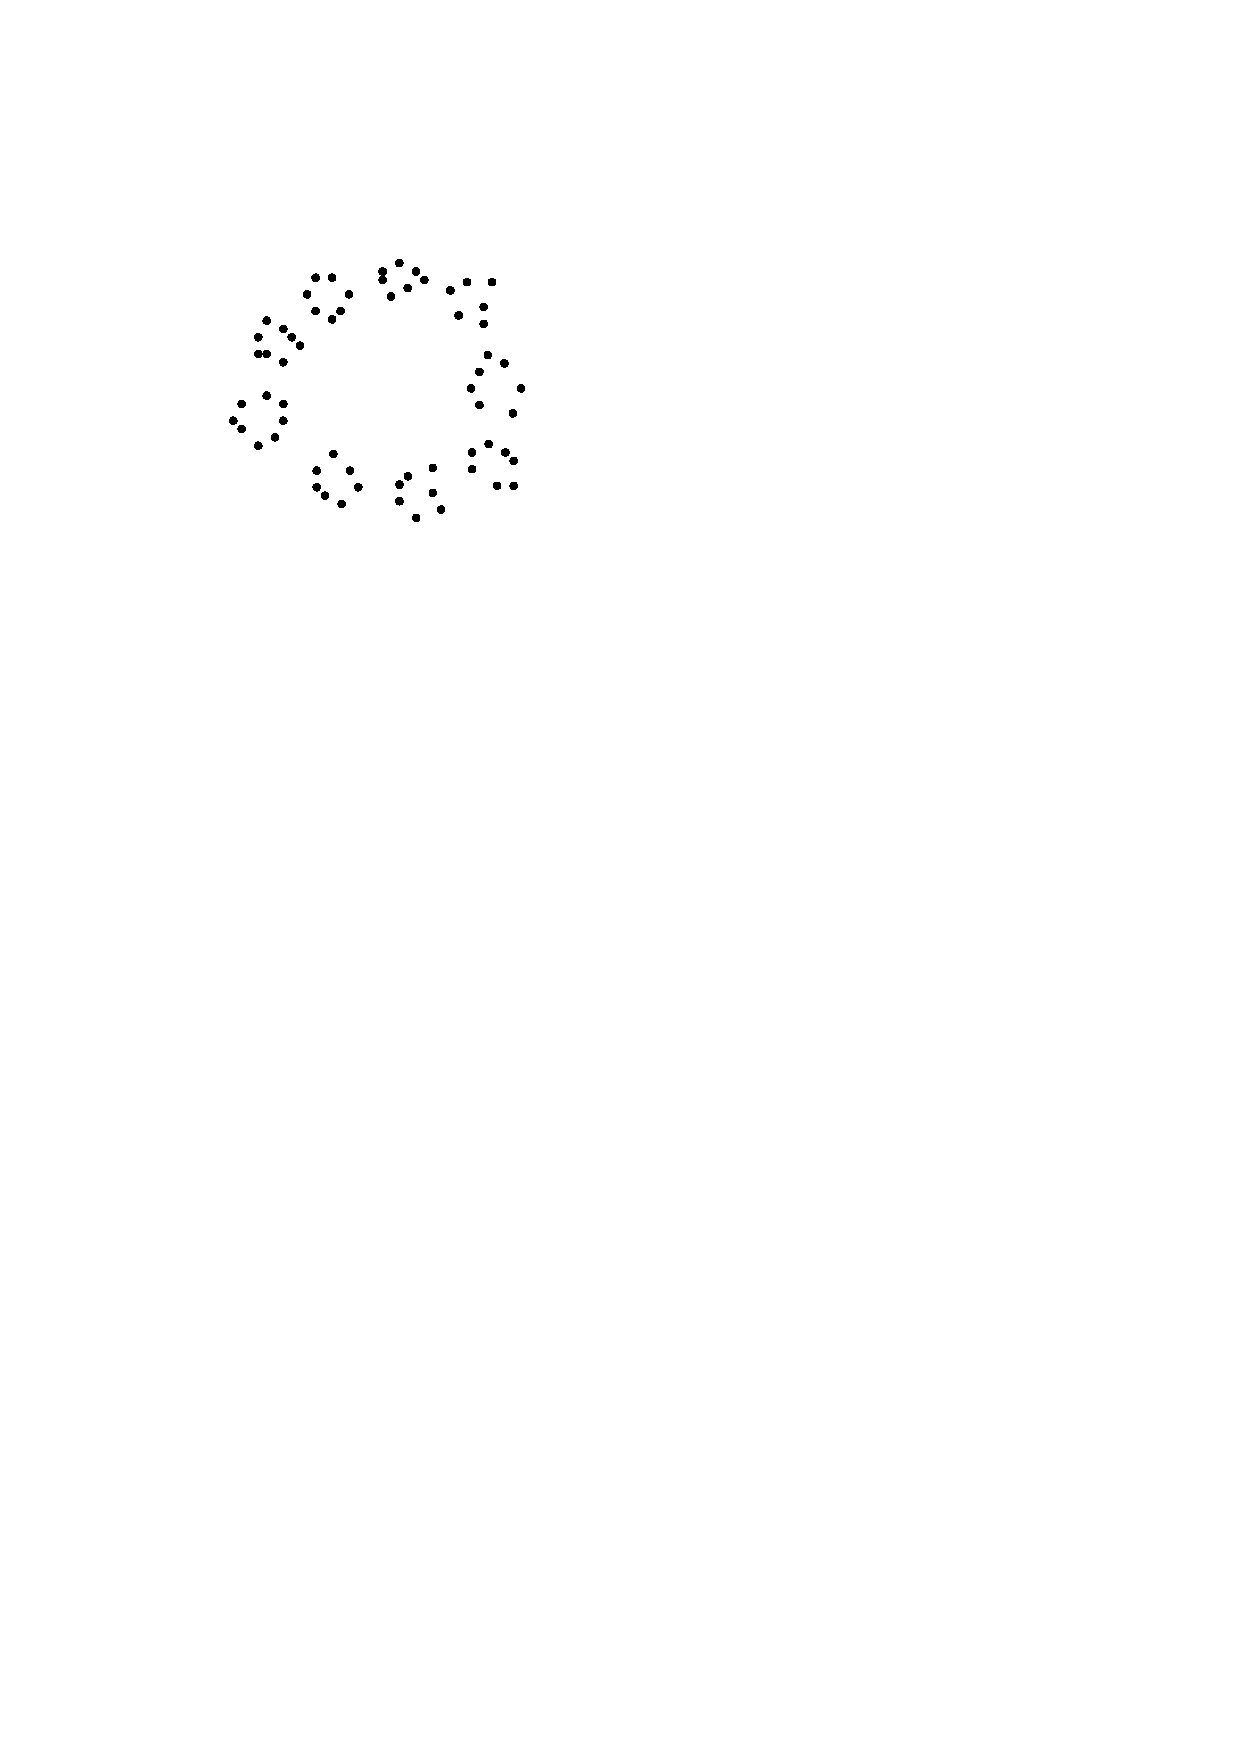
\includegraphics[width=.5\linewidth]{figures/ExampleScale}
  \captionof{figure}{
%Nuage de points avec diff\'erentes interprations topologiques d\'ependant de l'\'echelle. }
%A petite \'echelle, 
Ce nuage de points semble \'echantillonn\'e sur neuf cercle \`a petite \'echelle,
%\^etre l'union de neuf cercles, tandis qu'\`a une \'echelle plus grande, il s'agit plut\^ot d'
et sur un seul cercle \`a plus grande \'echelle.}
  \label{fig:echelle}
\end{minipage}
\end{figure}

%\begin{figure}
%\centering
%\begin{minipage}{.7\textwidth}
%  \centering
%  
\includegraphics[width=.9\linewidth]{figures/ExampleDeformation}
%  \captionof{figure}{Deformations of a circle.}
%A 1-dimensional hole is present in all of these deformations of the circle.}
%  \label{fig:deform}
%\end{minipage}%
%\begin{minipage}{.3\textwidth}
%  \centering
%  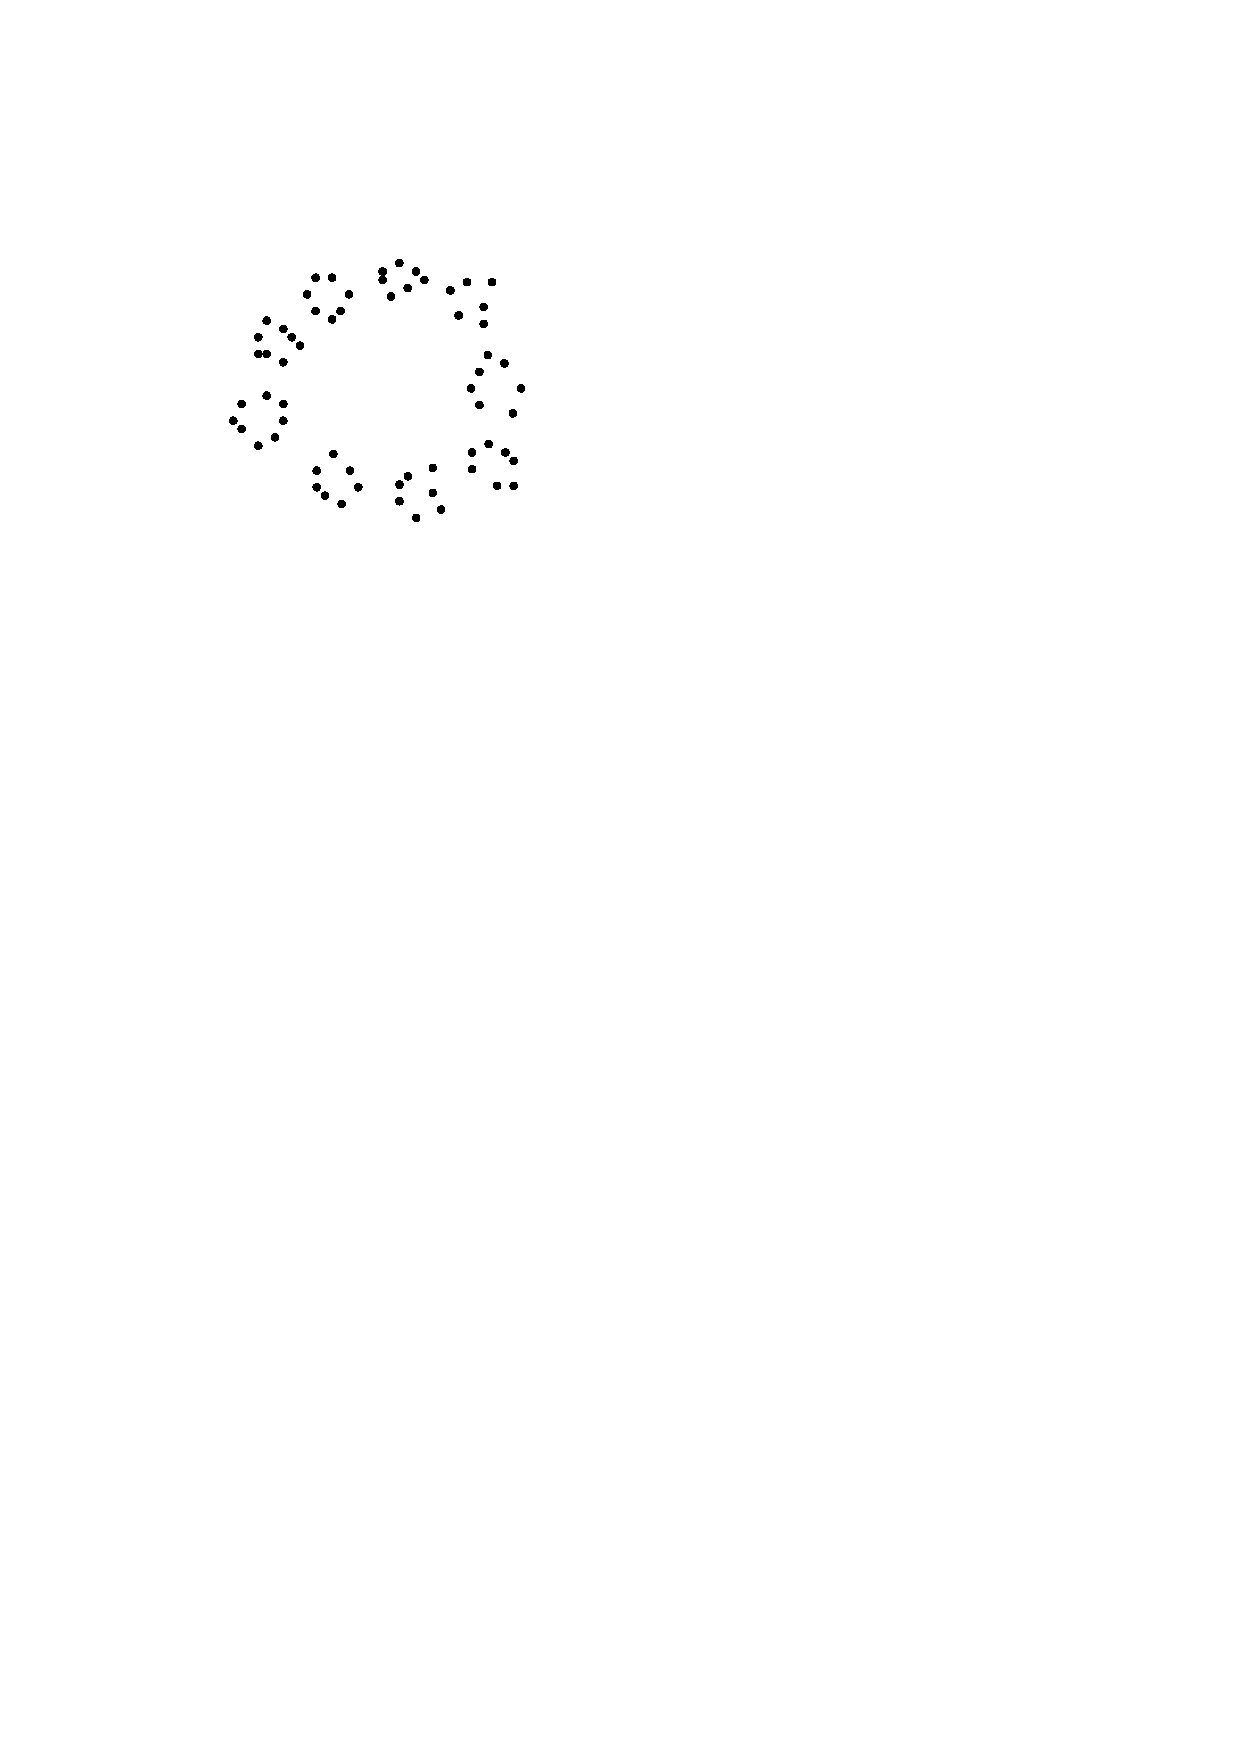
\includegraphics[width=.5\linewidth]{figures/ExampleScale}
%  \captionof{figure}{Point cloud with different topological features depending on the scale.}
%It is unclear in this example what the geometric underlying object is. At small scale, it seems to be a union 
%of nine circles, whereas it would rather be a single disk at a larger scale.}
%  \label{fig:scale}
%\end{minipage}
%\end{figure}

De mani\`ere similaire, les composantes connexes, cavit\'es, et trous de dimension sup\'erieure sont des attributs topologiques.
Dans l'optique de formaliser la pr\'esence de tels attributs (en toute dimension), {\em la th\'eorie de l'homologie}, 
a \'et\'e d\'evelopp\'ee au 19e et au d\'ebut du 20e si\`ecle.
Elle se pr\'esente comme un encodage alg\'ebrique de l'information topologique.
L'homologie d'un espace est une famille de groupes ab\'eliens (un pour chaque dimension), dont les \'el\'ements sont des combinaisons
lin\'eaires des trous de l'espace.

Cependant, les groupes d'homologie ne %peuvent pas \^etre utilis\'es en tant que tels comme 
sont pas des descripteurs topologiques tr\`es performants en tant que tels, la raison principale 
\'etant que les donn\'ees prennent souvent la forme de nuages de points, dont les groupes d'homologie ne sont pas informatifs : 
chaque point du nuage est un g\'en\'erateur du groupe d'homologie en dimension 0, puisque l'homologie en dimension 0 compte les
composantes connexes, et tous les groupes d'homologie de dimension sup\'erieure sont triviaux puisque le nuage n'a aucun trou.
Evidemment, le nuage de points peut tout de m\^eme refl\'eter de l'information topologique - par exemple s'il est \'echantillonn\'e 
sur un objet g\'eom\'etrique comme un cercle, une sph\`ere ou un tore. La question devient ainsi celle de l'\'echelle avec laquelle
observer les donn\'ees, comme illustr\'e dans la Figure~\ref{fig:echelle}. %, dans laquelle l'objet g\'eom\'etrique sous-jacent est ambigu.



%Similarly, connected components, cavities
%and higher-dimensional holes are topological features. In order to formalize the presence of such holes (in any dimension), 
%the so-called {\em homology} was developed in the 19th and the beginning of the 20th century as an algebraic encoding of such topological information. 
%Basically, the homology of a space is a family of algebraic groups
%(one for each topological dimension), whose elements are linear combinations of the space's holes.

%However, it turns out that the homology groups themselves cannot be used per se as topological descriptors. The main reason
%is that data often comes in the form of point clouds in data analysis, and the homology groups are not informative for such objects:
%each point of the cloud is a generator of the 0-dimensional homology group, since 0-dimensional homology is concerned with connected 
%components, and all higher-dimensional homology groups are trivial since the point cloud has no holes.
%However, it may happen that the data still contains topological information; 
%for instance if the point cloud is a sampling of a geometric underlying object such as
%a circle, a sphere or a torus. 
%Hence, the question that raises is that of the scale to which one should look at the data,
%as illustrated in Figure~\ref{fig:scale}, in which it is unclear what the geometric underlying object is. 
%At small scale, it seems to be a disjoint union of nine circles, whereas it would rather be a single circle at a larger scale.

%\begin{figure}[h]\centering
%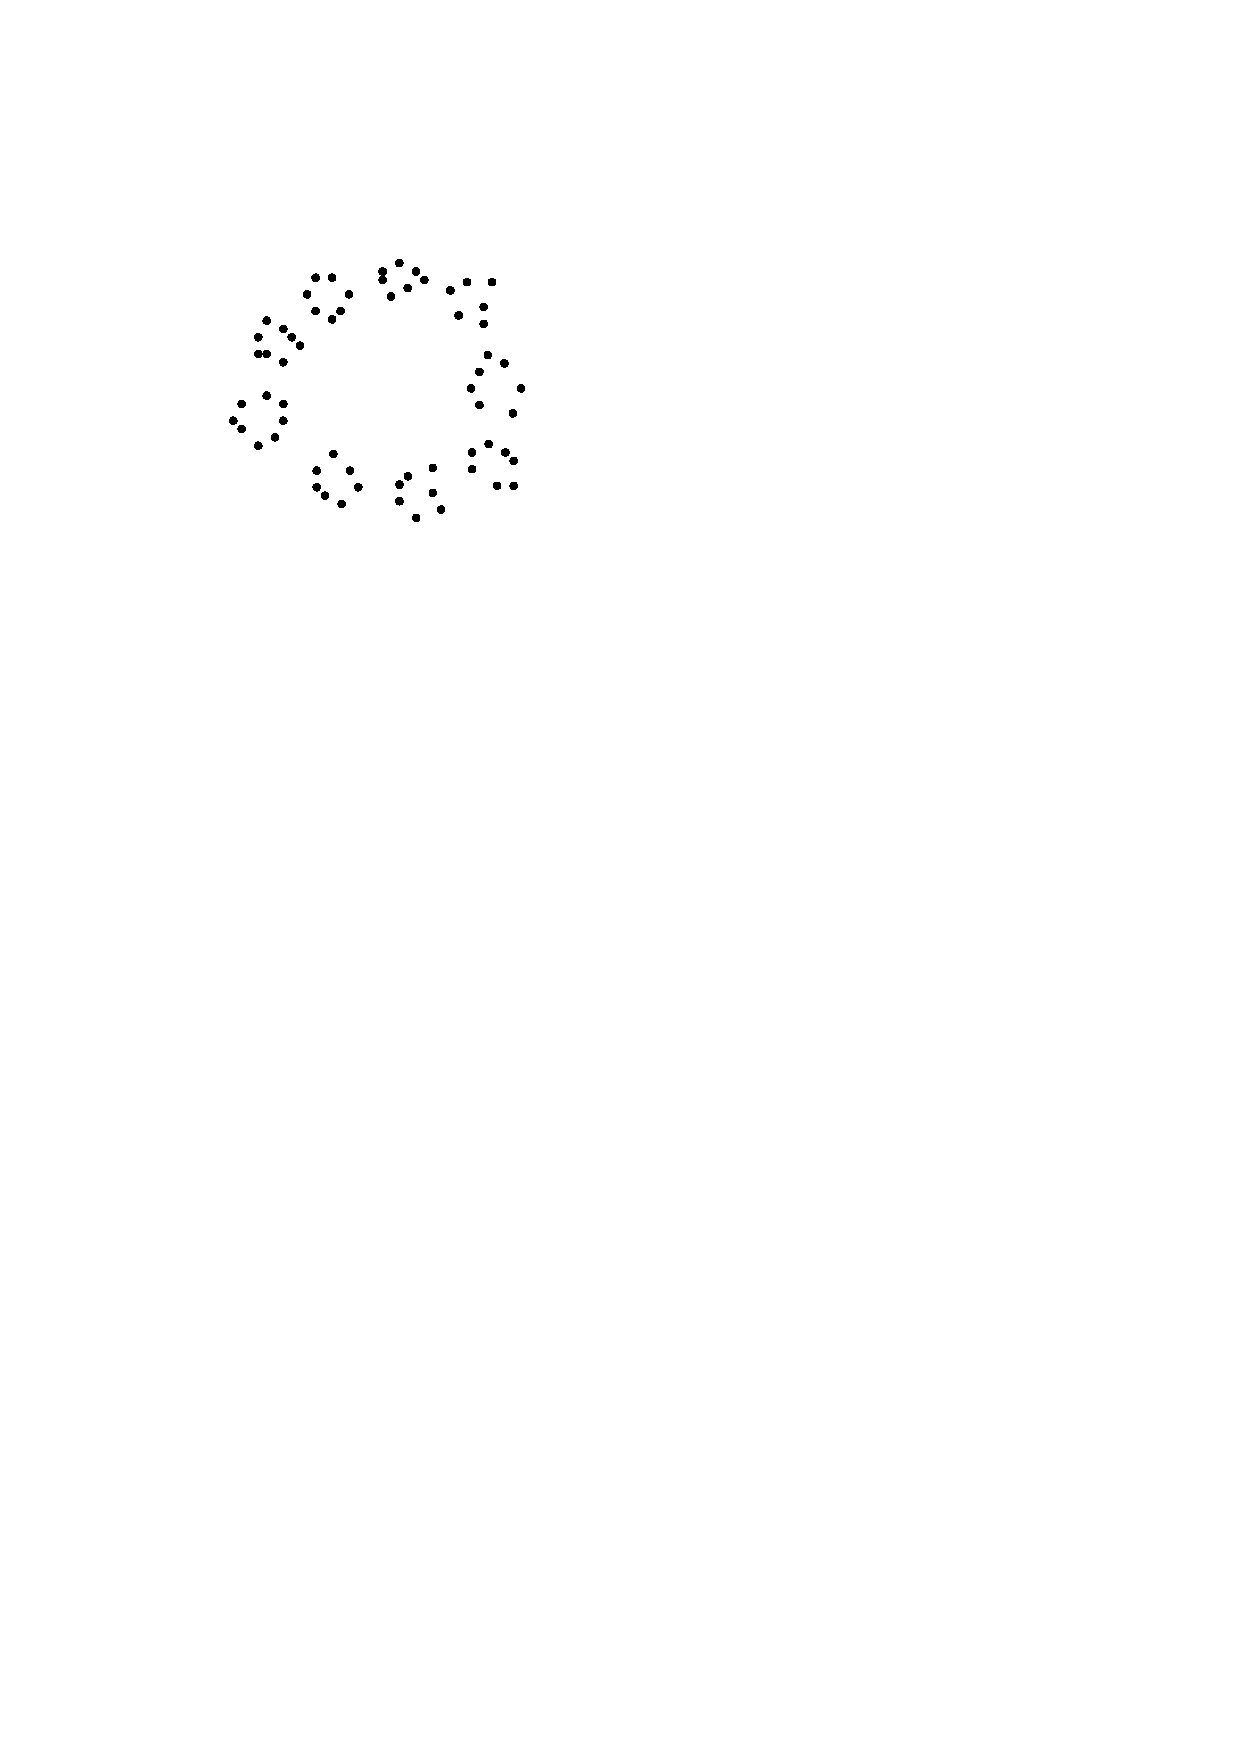
\includegraphics[height=2cm]{figures/ExampleScale}
%\caption{\label{fig:scale} It is unclear in this example what the geometric underlying object is. At small scale, it seems to be a union 
%of nine circles, whereas it would rather be a single disk at a larger scale.}
%\end{figure}



L'analyse de donn\'ees topologiques fournit deux constructions : les diagramme de persistance, qui synth\'etisent l'information topologique
\`a toutes les \'echelles, et les Mappers, qui encodent plus d'information g\'eom\'etrique \`a \'echelle fix\'ee.

%Topological data analysis provides two constructions:    
%the {\em persistence diagram}, which summarizes the topological information at all possible scales, and the {\em Mapper},
%which encodes more information, but at a fixed scale.

\paragraph*{Diagrammes de persistance.} Puisque chaque \'echelle fournit des informations topologiques pertinentes,
l'id\'ee de l'homologie persistante est d'encoder l'homologie du nuage de points \`a toutes les \'echelles. Consid\'erons
la base de donn\'ees de la Figure~\ref{fig:donnees}, contenant des images \`a 128 $\times$ 128 pixels, vus comme
des vecteurs en dimension 16 384, o\`u chaque coordonn\'ee est le niveau de gris d'un pixel.
%Puisque ces images repr\'esentent le m\^eme objet vus sous des angles diff\'erents, 
Puisque la cam\'era a tourn\'e autour de l'objet,
il s'ensuit qu'\`a petite \'echelle, les donn\'ees
semblent \^etre r\'eparties en petits groupes, tandis qu'\`a \'echelle plus grande, elles semblent \'echantillonn\'ees sur un cercle
(plong\'e dans $\R^{16384}$).

%\paragraph*{Persistence diagrams.} 
%Since several different scales may contain different topological information, the idea of persistent homology
%is to encode the homology of the point cloud at all possible scales. Consider the dataset of Figure~\ref{fig:dataset},
%containing images with 128 $\times$ 128 pixels, seen as 16,384-dimensional vectors, where each coordinate is the grey scale value of a pixel.
%Since these images represent the same object taken at different angles, it follows that, at a small scale, the data looks 
%composed of small clusters, each of which characterizing a specific angle, whereas at a larger scale, 
%the data seems to be sampled on a circle (embedded in $\R^{16,384}$).

\begin{figure}[h]\centering
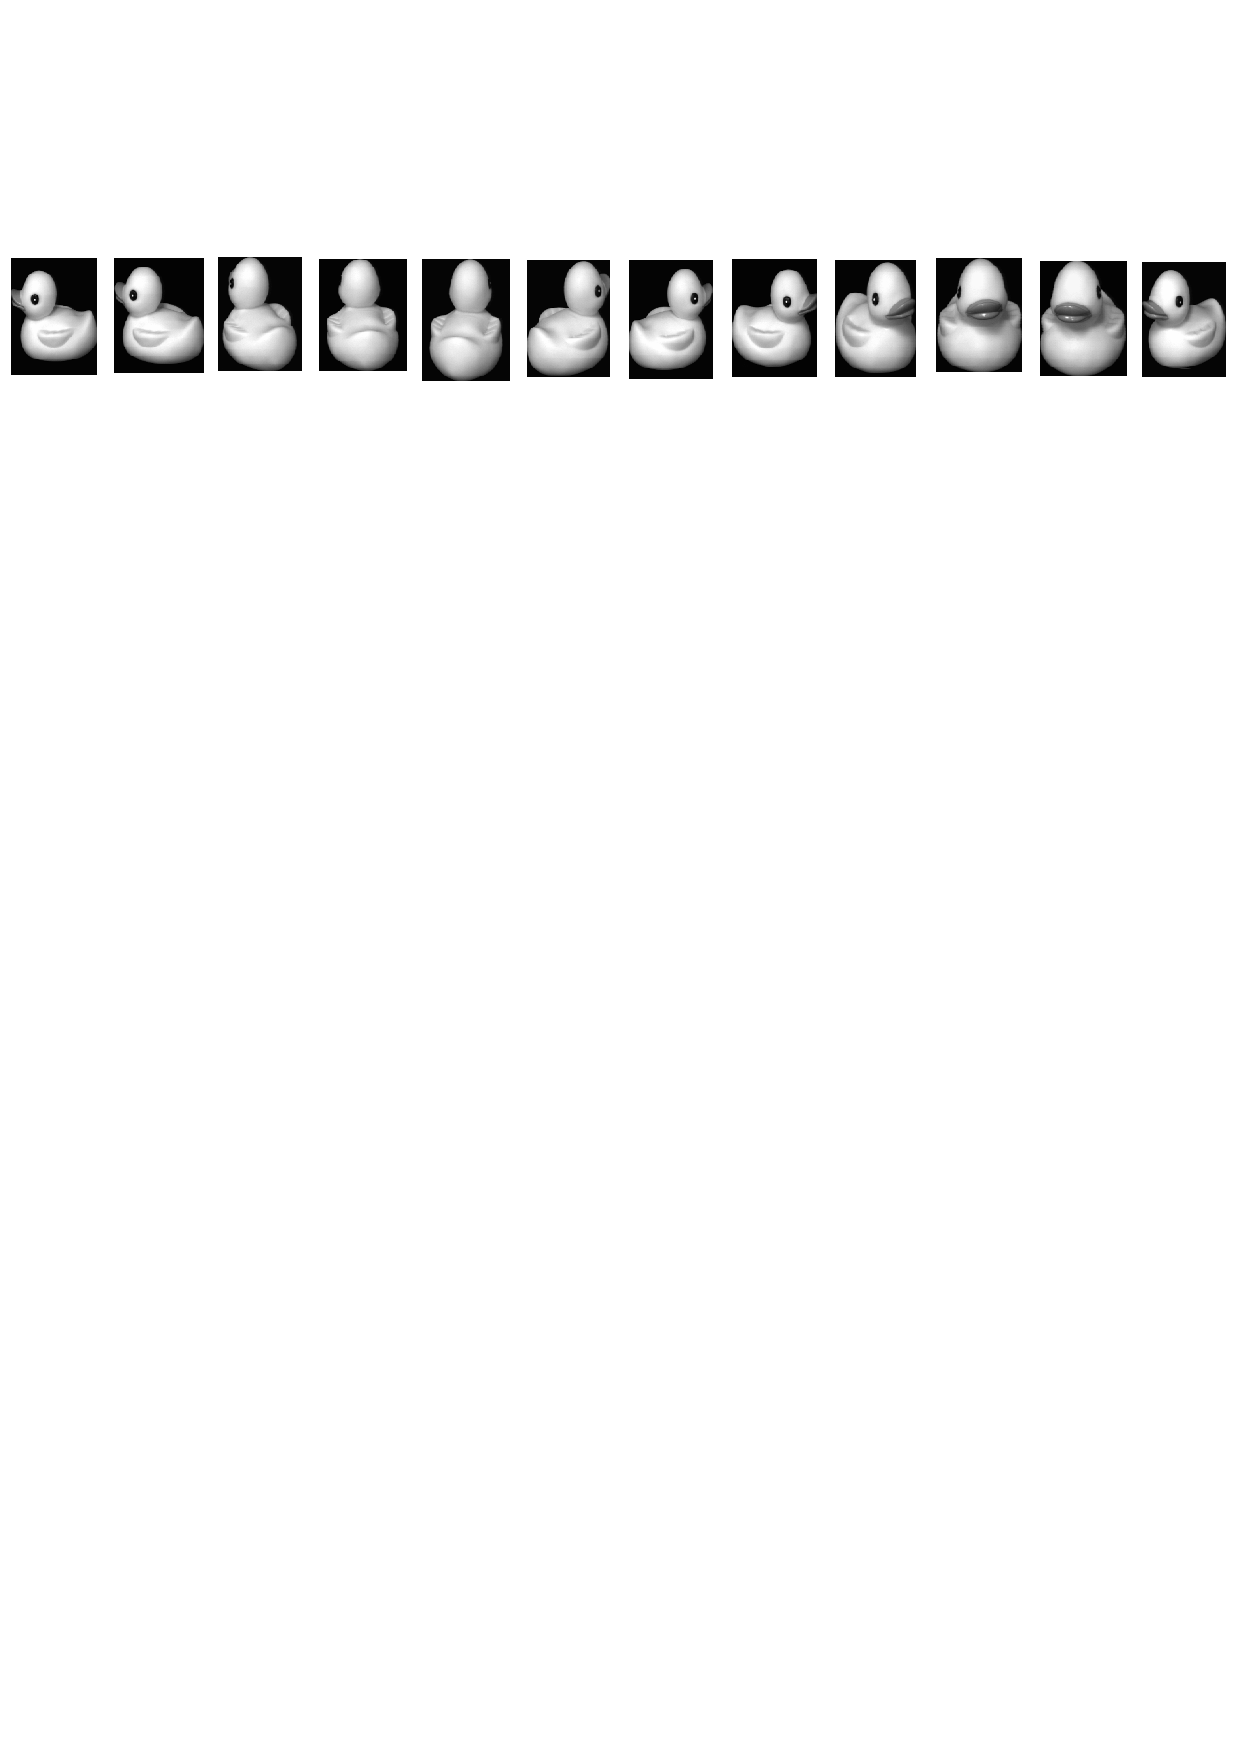
\includegraphics[width=\textwidth]{figures/ExampleDataset}
\caption{\label{fig:donnees} Une base de donn\'ees d'images.}
\end{figure}

%\begin{figure}[h]\centering
%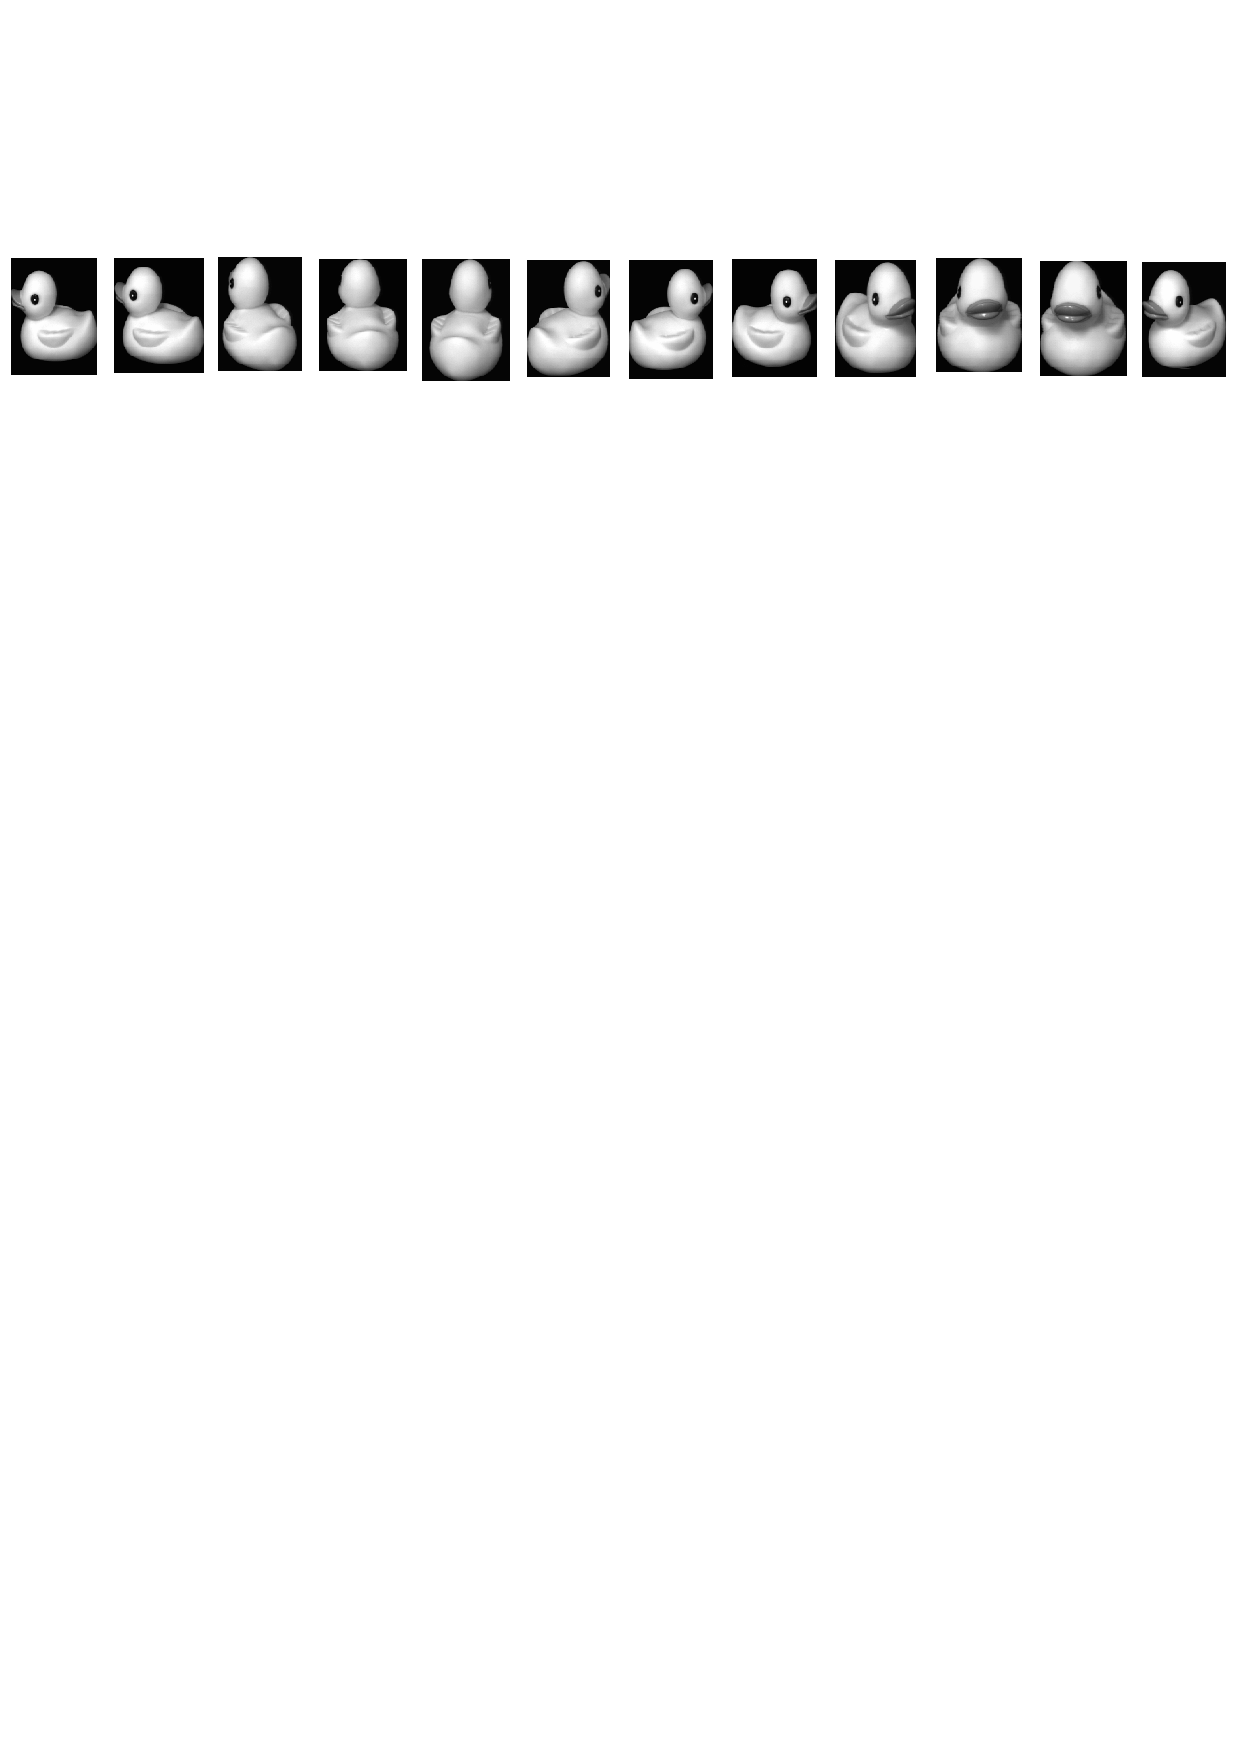
\includegraphics[width=\textwidth]{figures/ExampleDataset}
%\caption{\label{fig:dataset} A dataset of images.}
%\end{figure}

Pour synth\'etiser cette information, on peut faire grossir des boules centr\'ees sur les points de donn\'ees.
Consid\'erons trois rayons diff\'erents pour ces boules : un petit $\alpha$, un l\'eg\`erement plus grand $\beta$ et un
beaucoup plus grand $\gamma$, comme montr\'e dans la Figure~\ref{fig:ExemplePersistance}.

%To summarize this information, the idea is to grow balls centered on each point of the dataset. 
%Let us look at three different radius values: a small one $\alpha$, an slightly larger intermediate one $\beta$ and
%a very larger one $\gamma$ for these balls, as displayed in Figure~\ref{fig:ExamplePersistence}.

%\begin{figure}[h]\centering
%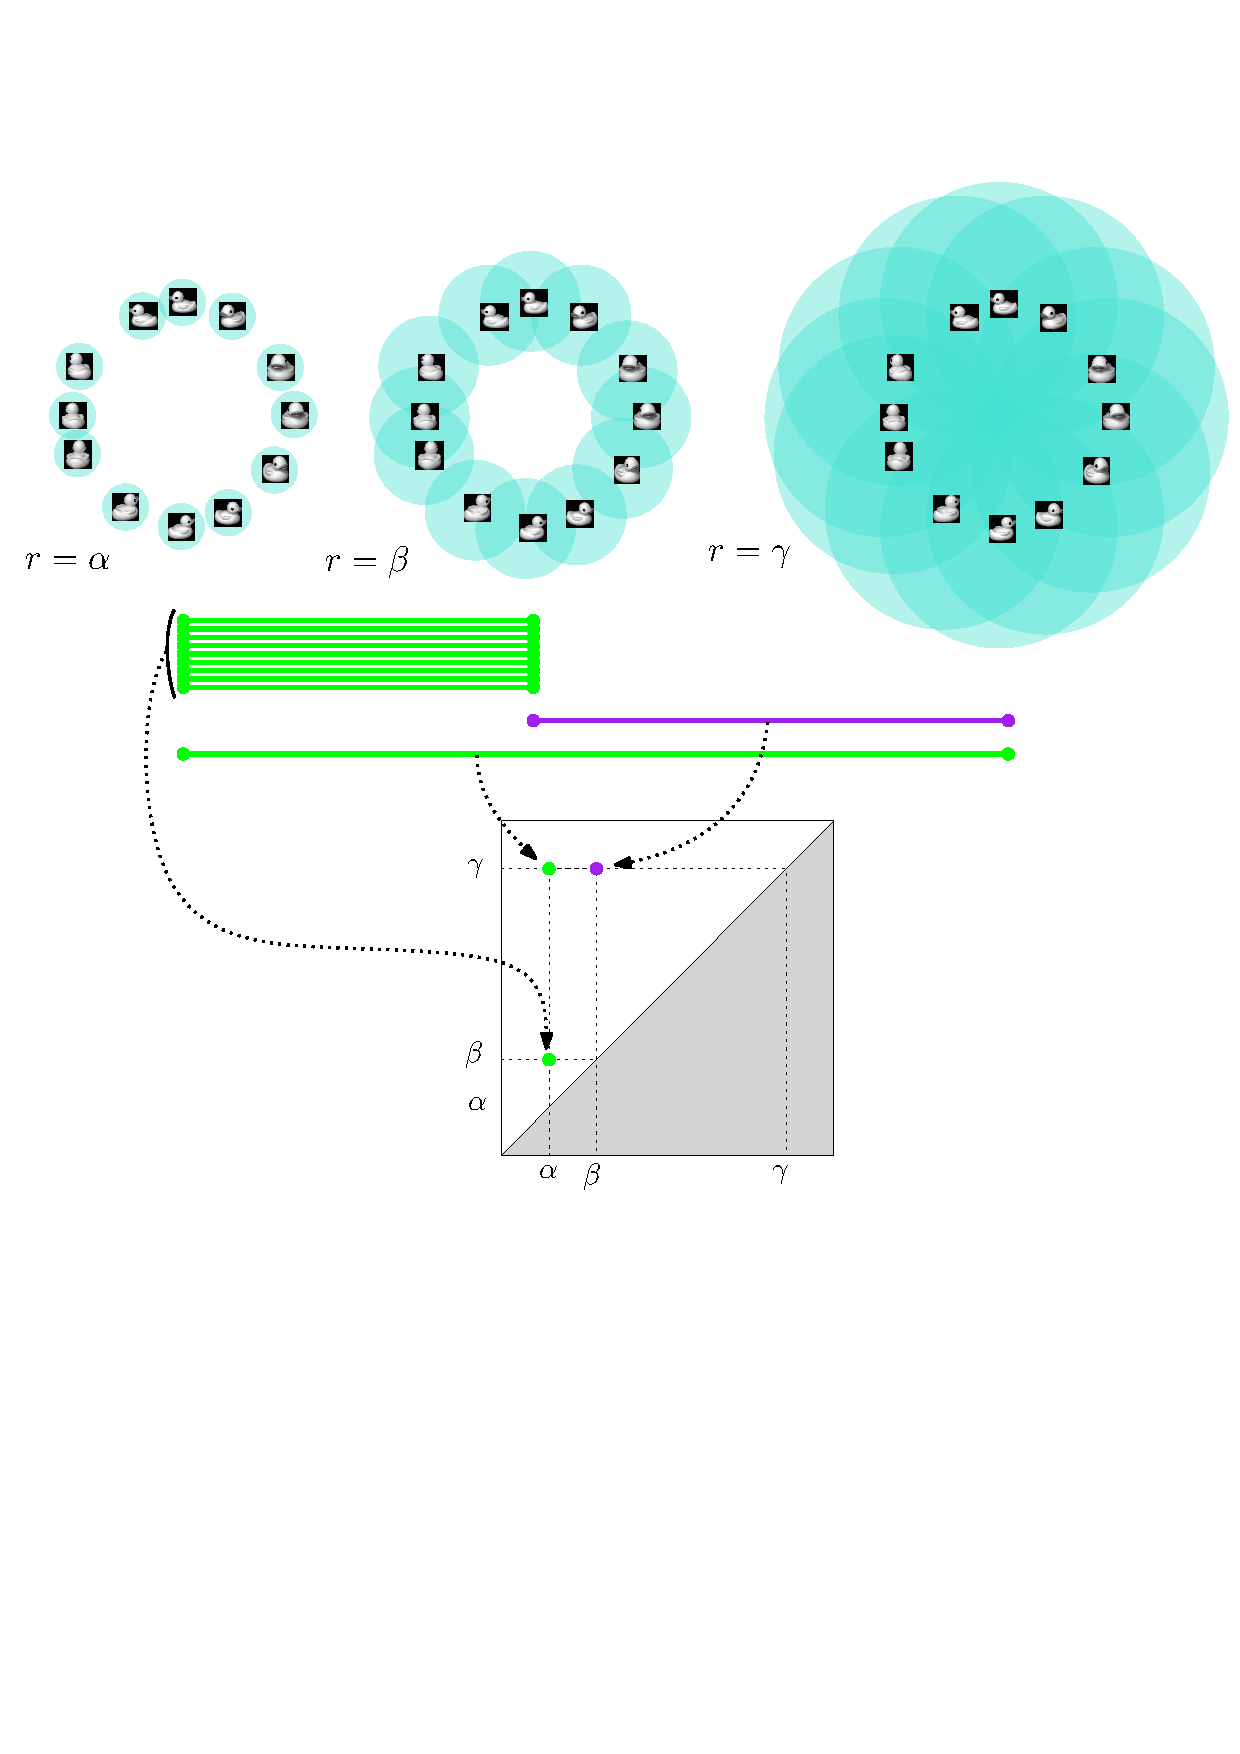
\includegraphics[width=0.8\textwidth]{figures/ExamplePersistence}
%\caption[Persistence diagrams induced by growing balls]{\label{fig:ExamplePersistence} Three difference unions of balls centered on images seen as vectors in high-dimensional Euclidean space.
%The appearance and disappearance of topological features like connected components or holes is recorded and stored in the so-called {\em persistence diagram},
%in which green points represent 0-dimensional features and purple points represent 1-dimensional ones.}
%\end{figure}	

\begin{figure}[h]\centering
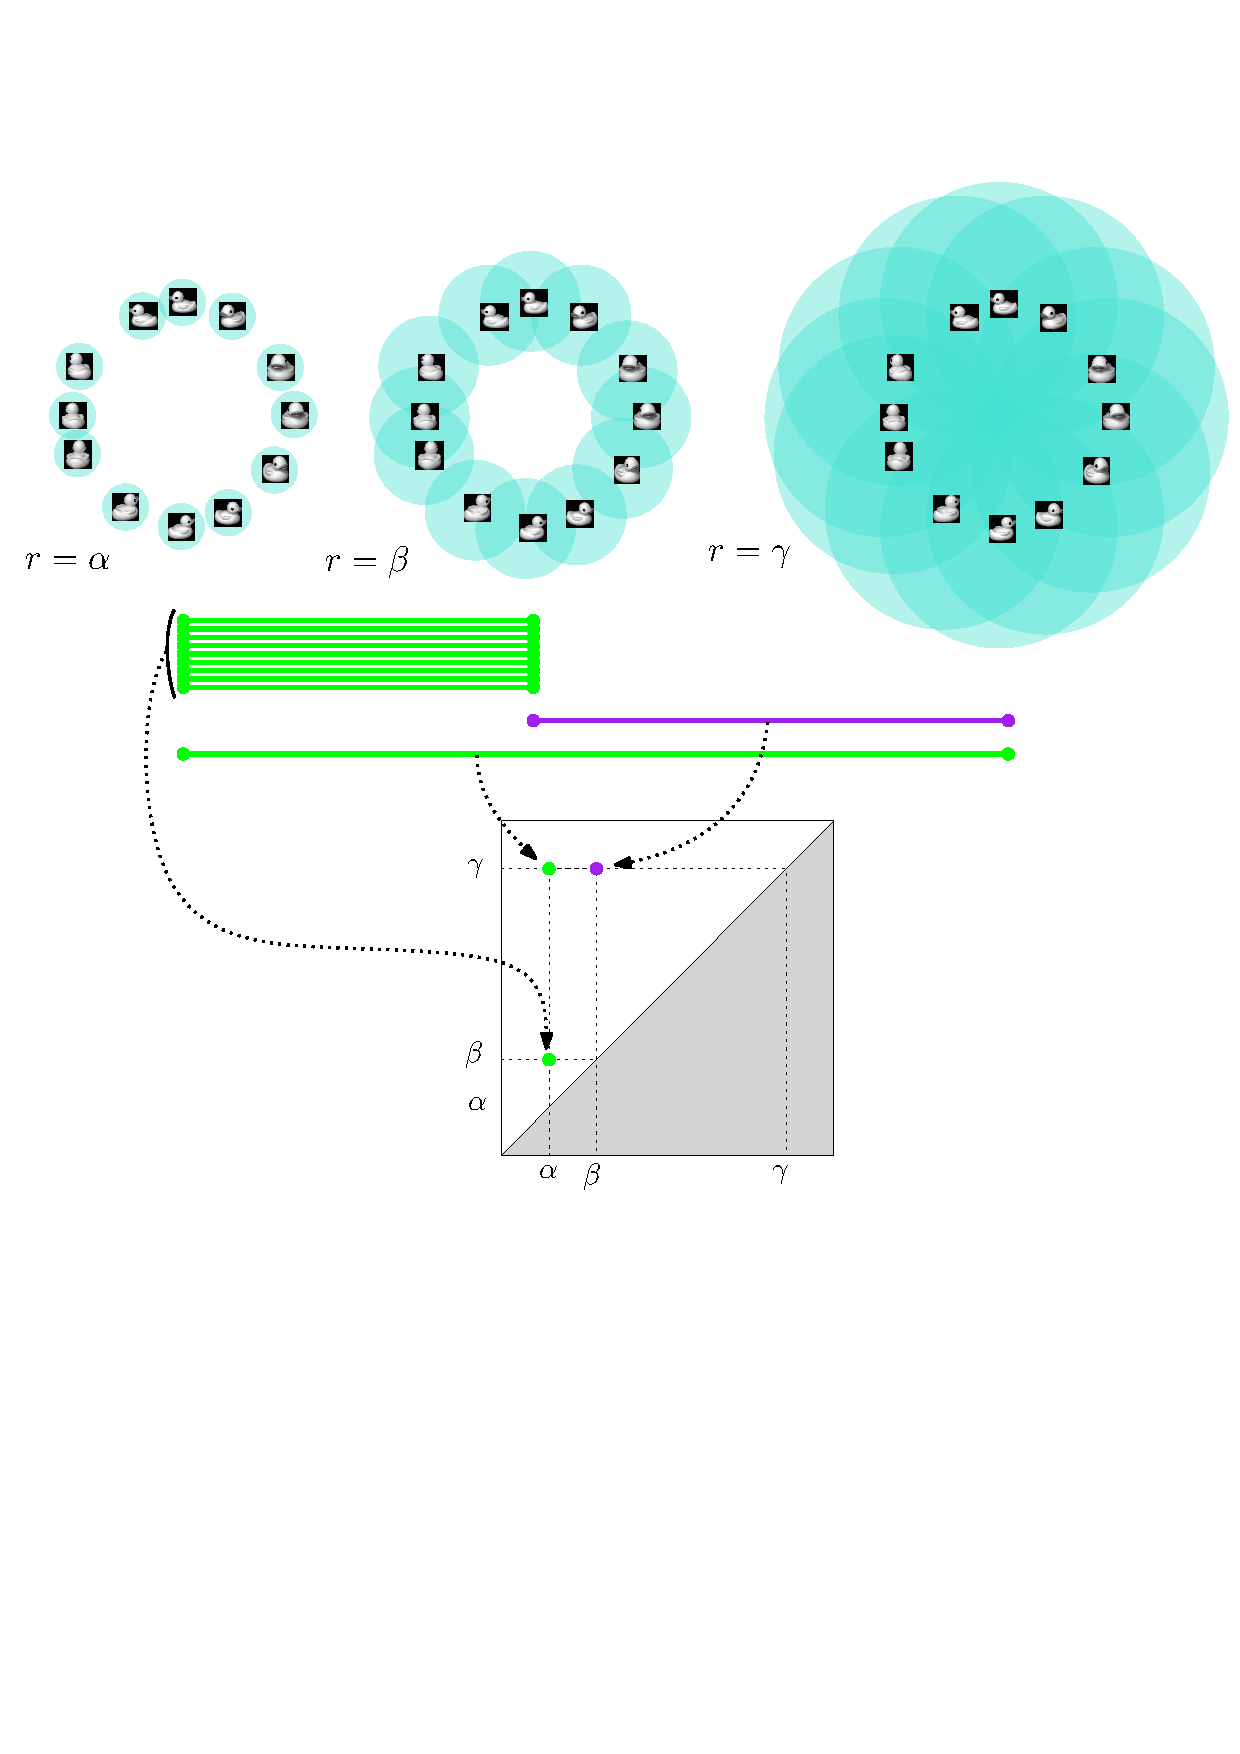
\includegraphics[width=0.8\textwidth]{figures/ExamplePersistence}
\caption[Diagrames de persistance induit par des boules grossissantes]{\label{fig:ExemplePersistance} 
Trois diff\'erentes unions de boules centr\'ees sur des images vus comme des vecteurs dans un espace Euclidien de grande dimension.
L'apparition et la disparition d'attributs topologiques, comme des composantes connexes ou des trous, est enregistr\'ee dans un {\em diagramme de persistance},
dans lequel les points repr\'esentant des attributs en dimension 0 sont en vert, et ceux repr\'esentant des attributs en dimension 1 sont en violet.}
\end{figure}

Quand le rayon des boules vaut $\alpha$, l'union des boules est simplement l'union de dix composantes connexes, dont l'homologie en dimension 1
et sup\'erieure est triviale.
Cependant, quand le rayon devient $\beta$, l'union des boules a l'homologie d'un cercle, dont le trou en dimension 1
devient rempli quand le rayon devient $\gamma$. On dit que les composantes connexes sont n\'ees \`a la valeur $\alpha$,
et neuf sont mortes, c'est-\`a-dire se sont fait relier \`a la dixi\`eme, \`a la valeur $\beta$. De la m\^eme mani\`ere, le trou en dimension 1
est apparu au rayon $\beta$, et a disparu au rayon $\gamma$. Enfin, la dixi\`eme composante connexe est apparue au rayon $\alpha$
et a persist\'e jusqu'au rayon $\gamma$. Cette information est encod\'ee dans le {\em diagramme de persistance}, qui est un multi-ensemble
\footnote{Un multi-ensemble est une g\'en\'eralisation d'un ensemble, dans laquelle les points ont des multiplicit\'es.}
% pouvant contenir plusieurs fois le m\^eme point.} 
de points, chacun repr\'esentant
un attribut topologique, et ayant les rayons de naissance et de mort comme coordonn\'ees.
La distance \`a la diagonale fournit une quantit\'e utile et interpr\'etable dans les diagrammes de persistance. En effet, si un point est loin
de la diagonale, alors son ordonn\'ee est largement sup\'erieur \`a son abscisse, ce qui signifie que l'attribut topologique correspondant
\'etait pr\'esent dans l'union des boules pour une large gamme de rayons diff\'erents, indiquant ainsi que l'attribut topologique
a des chances d'\^etre pr\'esent dans l'objet sous-jacent, et d'\^etre une information pertinente. Au contraire, les points proches de la diagonale
repr\'esentent des attributs qui ont disparu rapidement apr\`es \^etre apparus. Ces attributs \'ephem\`eres correspondent plut\^ot \`a du bruit ou des 
attributs de l'objet sous-jacent qui ne sont pas pertinents. C'est le cas par exemple des neuf composantes connexes de l'union des boules au rayon $\alpha$
dans la    Figure~\ref{fig:ExemplePersistance}, qui ont disparu au rayon $\beta$, proche de $\alpha$.
Il est \`a noter que nous avons \'expliqu\'e la construction dans le cas o\`u il n'y a que trois unions de boules, mais il est bien s\^ur possible
de construire un diagramme de persistance quand le rayon des boules augmente continument de $0$ \`a $+\infty$.
Dans ce cas, le trou de dimension 1 a une abscisse situ\'ee entre $\alpha$ et $\beta$ (car il n'est pas encore pr\'esent pour le rayon $\alpha$
et est d\'ej\`a l\`a au rayon $\beta$), et une ordonn\'ee situ\'ee entre $\beta$ et $\gamma$ (car il a d\'ej\`a disparu au rayon $\gamma$).
De m\^eme, toutes les composantes connexes ont pour abscisse $0$. Neuf d'entre elles\footnote{En fait, chaque point est une composante connexe au rayon $0$.} 
ont une ordonn\'ee comprise  entre $\alpha$ et $\beta$
et l'ordonn\'ee de la dixi\`eme est $+\infty$ puisqu'elle est toujours pr\'esente, quelque soit le rayon des boules.

%When the radius of the balls is $\alpha$,
%the union of balls is a just a union of ten connected components with trivial homology in dimension 1 and above.
%However, when the radius is $\beta$, the union of balls has the homology of a circle, whose 1-dimensional hole
%eventually gets filled in when the radius increases to $\gamma$. Hence, we say that the connected components were born at value $\alpha$,
%and nine of them died, or got merged to the tenth one, at radius $\beta$. Similarly, the 1-dimensional hole was born, or appeared, at value $\beta$ and
%died, or got filled in, at value $\gamma$. Finally, the tenth connected component appeared at radius $\beta$ and remained all the way until radius $\gamma$.
%This is summarized in the {\em persistence diagram}, which is a multiset
%\footnote{A multiset is a set where one can find the same element multiple times.} of points, each of which 
%representing a topological feature and having the birth and death radii as coordinates. 
%The distance to the diagonal is a useful interpretable quantity in persistence diagrams. Indeed, if a point is far from the diagonal, then 
%its ordinate, or death radius, is much larger than its abscissae, or birth radius. This means that the corresponding topological feature was
%present in the union of balls for a large interval of radii, suggesting that the feature is likely to be present in the underlying object, and thus significant.
%On the contrary, points close to the diagonal represent features that disappeared quickly after their appearance. These fleeting features are 
%likely to be nonsignificant features or noise artifacts. Consider for instance the nine connected components in the union of balls of 
%radius $\alpha$ in Figure~\ref{fig:ExamplePersistence}, which disappeared at radius $\beta$ slightly larger than $\alpha$.

Les diagrammes de persistance peuvent en faire \^etre d\'efinis beaucoup plus g\'en\'eralement.
%M\^eme si nous avons pr\'esent\'e un exemple sur un  nuage de points, les diagrammmes de persistance peuvent \^etre d\'efinis et construits
%\`a partir d'une tr\`es grande vari\'et\'e d'espaces
 - m\^eme si l'interpr\'etation en terme d'\'echelle n'est plus forc\'ement pertinente.
Tout ce qui est requis est une famille d'espaces intriqu\'es les uns dans les autres, appel\'ee {\em filtration}, 
c'est-\`a-dire une famille $\{X_\alpha\}_{\alpha\in A}$,
o\`u $A$ est un ensemble d'indices totalement ordonn\'es, telle que $\alpha\leq\beta\Rightarrow X_\alpha\subseteq X_\beta$.
La construction du diagramme de persistance est alors la m\^eme, c'est-\`a-dire l'enregistrement de l'apparition et de la disparition
d'attributs topologiques quand on parcourt $A$ par ordre croissant. Dans l'exemple pr\'ec\'edent, la filtration contient trois espaces, qui sont 
les trois diff\'erentes unions de boules, chaque union \'etant indic\'ee par le rayon de ses boules.
Il est clair dans ce cas que ces trois espaces sont intriqu\'es car une boule est toujours incluse dans la boule de m\^eme centre avec un rayon sup\'erieur.


%Even though we presented an example on a point cloud, persistence diagrams can be defined and built over much larger classes of spaces---even
%though the interpretation with scales may no longer be true.
%All that is needed is a family of spaces which is nested with respect to the inclusion, i.e. a family $\{X_\alpha\}_{\alpha\in A}$, where 
%$A$ is an ordered index set, such that $\alpha\leq\beta\Rightarrow X_\alpha\subseteq X_\beta$.
%Then, the construction of persistence diagrams remains the same, i.e. keeping track of the appearance and disappearance of topological features
%as we go through all indices in ascending order.
%In the previous example, the correspondings spaces
%were the different unions of balls, each union being indexed by the radius of its balls.
%It is clear in this case that the spaces are nested since a ball
%is always included in the ball with same center and larger radius.

Une mani\`ere pratique de construire une filtration est d'utiliser les {\em sous-niveaux} d'une fonction continue \`a valeurs
r\'eelles $f$, c'est-\`a-dire les espaces de la forme $f^{-1}((-\infty,\alpha])$. En effet, il est \'evident que 
$f^{-1}((-\infty,\alpha])\subseteq f^{-1}((-\infty,\beta])$ pour tous $\alpha\leq\beta\in\R$. 
Par exemple, l'union des boules de rayon $r$ centr\'ees sur les points d'un nuage $P$ %: $\cup_{p\in P}B(p,r)$, 
est \'egale au sous-niveau de la fontion distance au nuage $P$ : $d_P^{-1}((-\infty,r])$, o\`u $d_P(x)=\min_{p\in P}d(x,p)$.
Ainsi, d\`es qu'une fonction continue \`a valeurs r\'eelles est \`a disposition, un diagramme de persistance peut \^etre construit, ce qui explique
pourquoi le diagramme de persistance est un descripteur prolifique.
%utilis\'e non seulement pour les bases de donn\'ees, mais aussi pour les points de donn\'ees eux-m\^emes, comme illustr\'e par 
Prenons par exemple l'image floue d'un z\'ero, affich\'ee dans le coin inf\'erieur droit de la Figure~\ref{fig:zeroflou},
pour laquelle le niveau de gris des pixels est utilis\'e comme fonction continue pour calculer un diagramme de persistance. De nouveau, on trouve deux points se distinguant 
des autres dans le diagramme de persistance, l'un repr\'esentant la composant connexe du z\'ero, et l'autre son trou de dimension 1. Le reste 
des points est engendr\'e par le bruit pr\'esent dans l'image.

%A common way to build such a family of nested spaces is to use the {\em sublevel sets} of a continuous scalar-valued function $f$, which are sets of the form
%$f^{-1}((-\infty,\alpha])$. Indeed, it is clear that $f^{-1}((-\infty,\alpha])\subseteq f^{-1}((-\infty,\beta])$ for any $\alpha\leq\beta\in\R$. 
%For instance, given a point cloud $P$, the unions of balls with radius $r$ centered on points of $P$: $\cup_{p\in P}B(p,r)$, 
%is equal to the sublevel set of the distance function to  $P$:
%$d_P^{-1}((-\infty,r])$,
%where $d_P(x)=\min_{p\in P}d(x,p)$.
%Hence, as soon as there is a continuous scalar-valued function at hand, a persistence diagram can be computed, which explains
%why the persistence diagram is a versatile descriptor that can be used not only for datasets, but also for data points. 
%Take for instance the blurry image of a zero in the down right corner of Figure~\ref{fig:blurryzero}, where
%the grey value function is used to compute the persistence diagram. Again, there are two points standing out
%in the persistence diagram, one representing the connected component of the zero, and the other representing 
%the 1-dimensional hole induced by the zero. All other points are noise. 

%\begin{figure}[h]\centering
%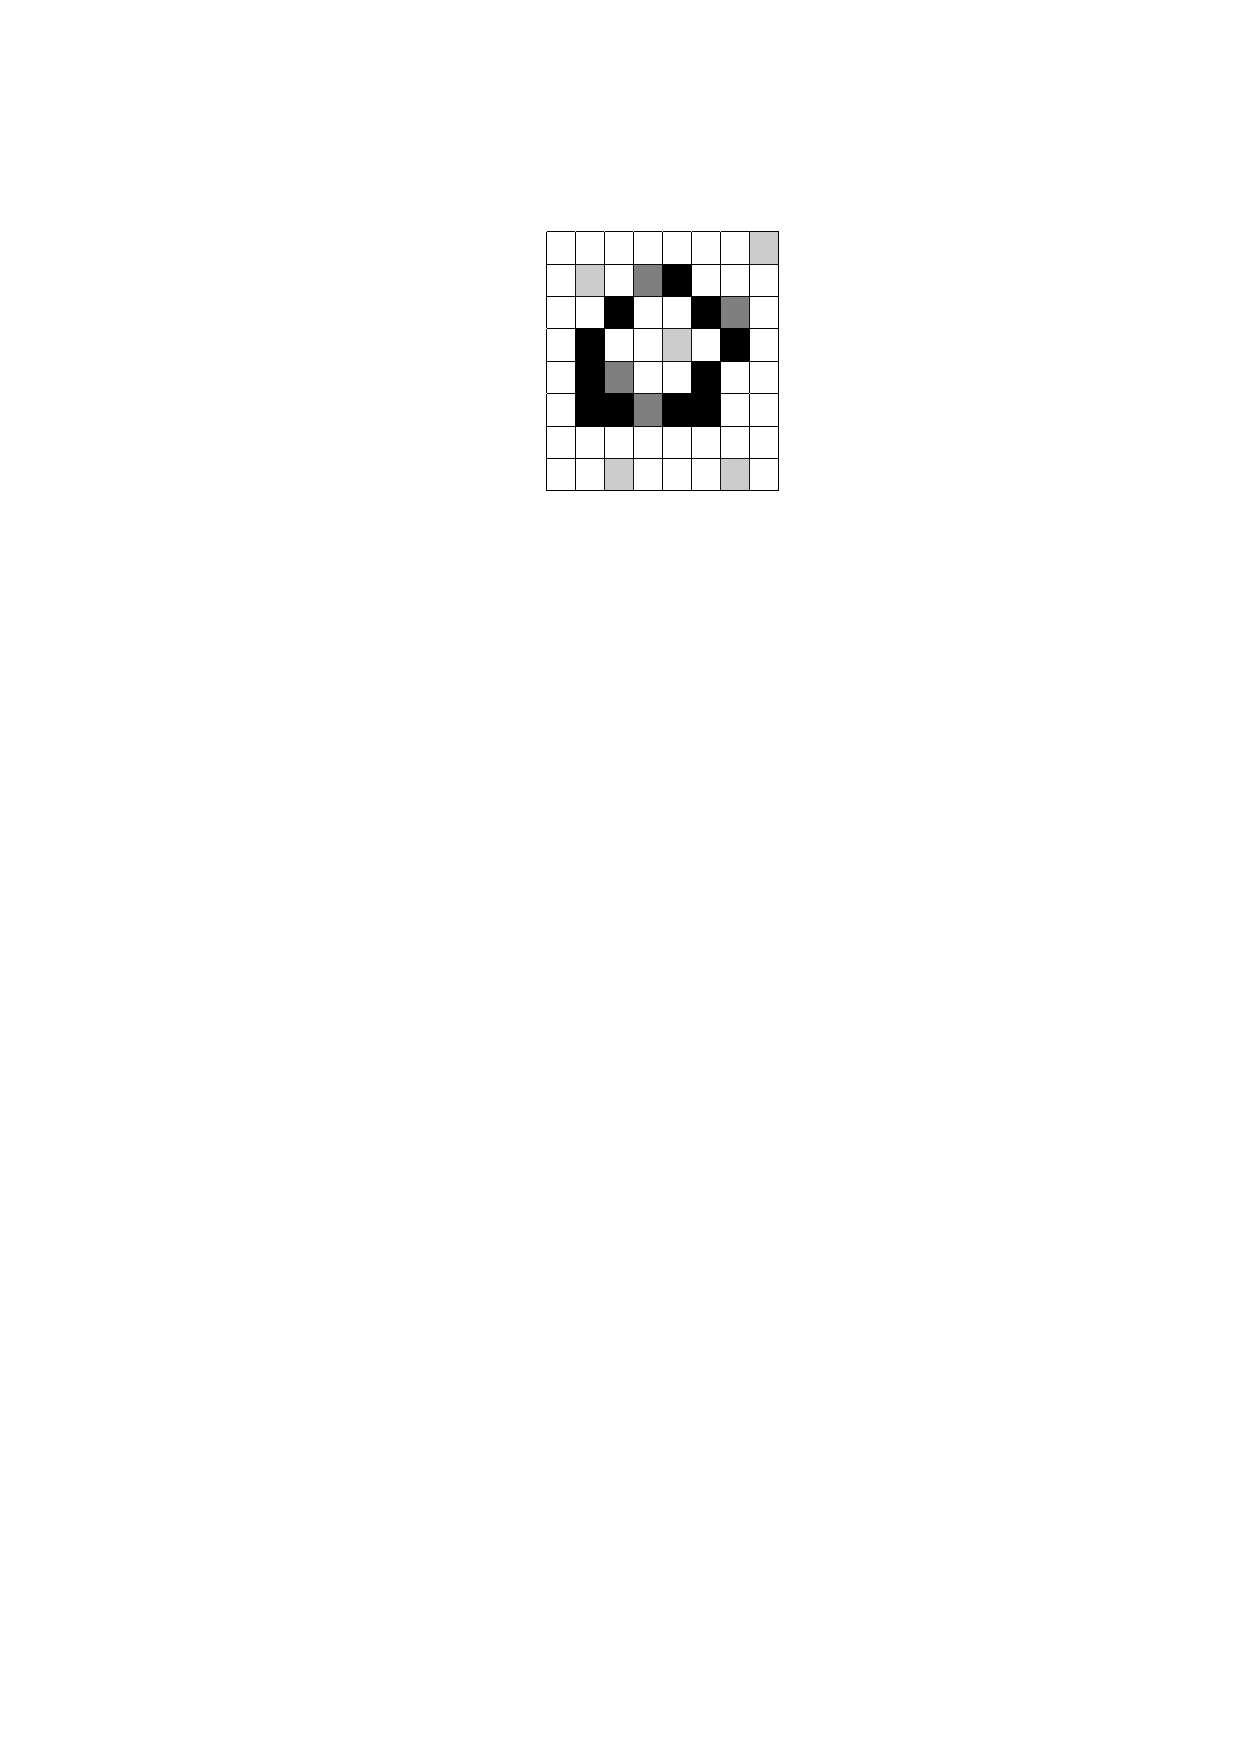
\includegraphics[width=5cm]{figures/ExampleImage}
%\caption{\label{fig:blurryzero}}
%\end{figure} 

\begin{figure}[h]\centering
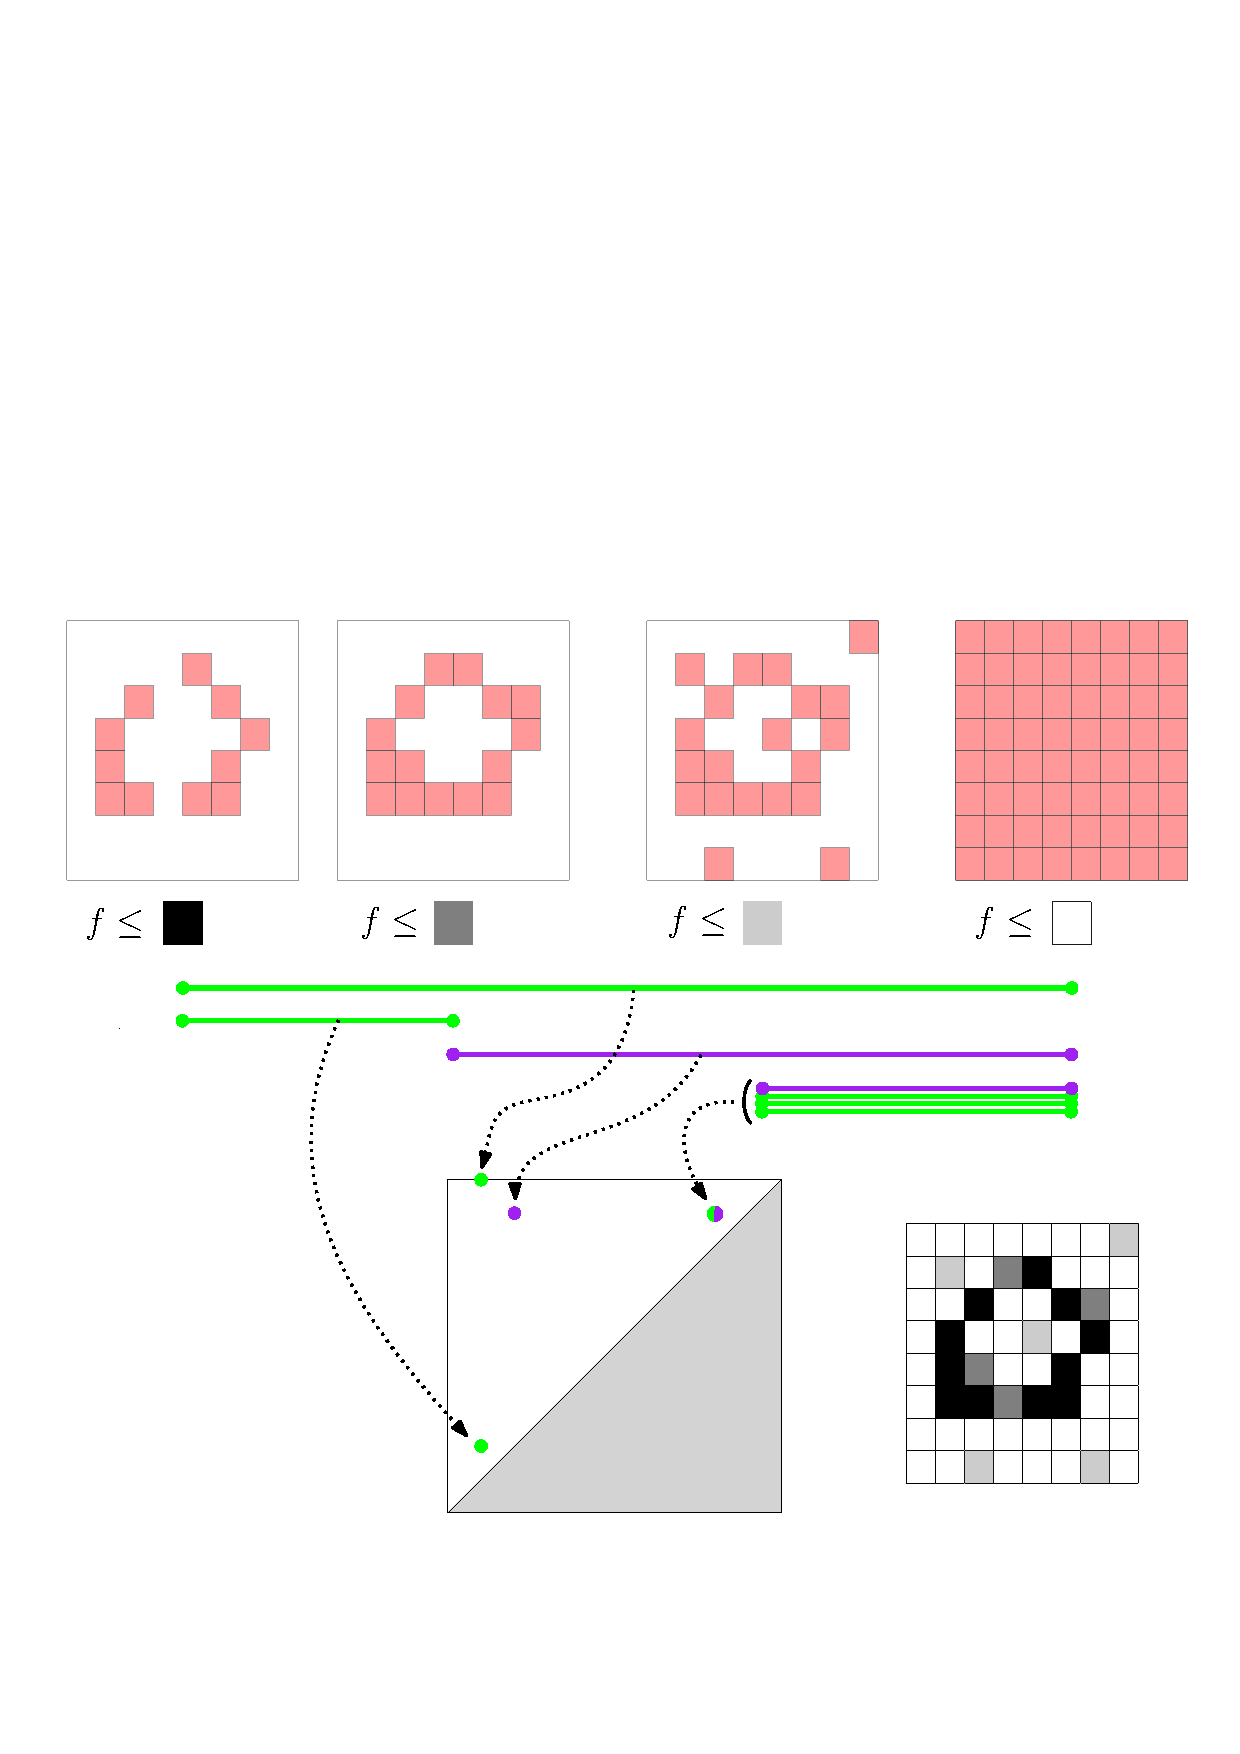
\includegraphics[width=0.8\textwidth]{figures/ExamplePersistence2}
\caption[Diagramme de persistance d'une image]{\label{fig:zeroflou} 
Autre exemple d'une construction de diagramme de persistance,
avec les sous-niveaux du niveau de gris des pixels d'une image floue d'un z\'ero.}
\end{figure}

%\begin{figure}[h]\centering
%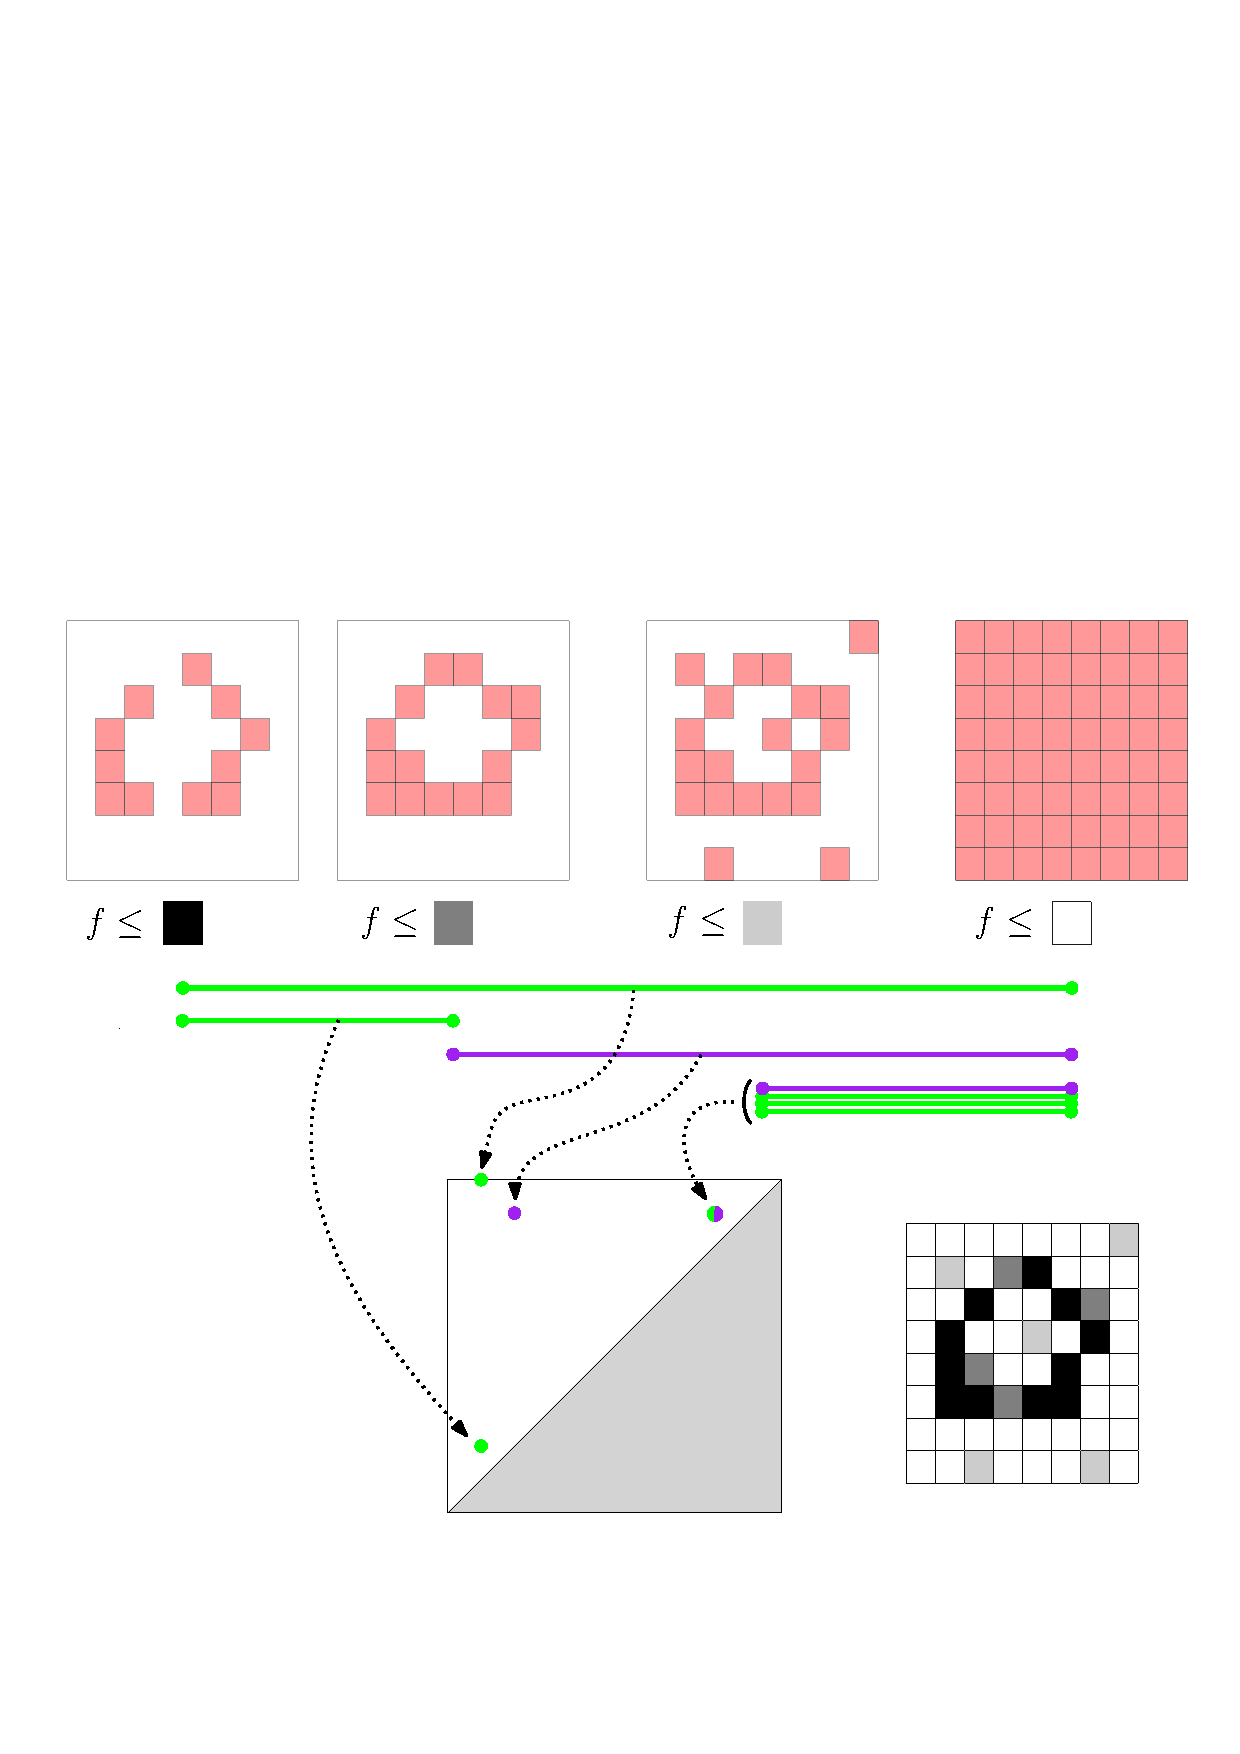
\includegraphics[width=0.8\textwidth]{figures/ExamplePersistence2}
%\caption[Persistence diagram of image]{\label{fig:blurryzero} Another example of a persistence diagram construction with the sublevel sets of the 
%grey value function defined on a blurry image of a zero.}
%\end{figure}	

Une des raisons pour lesquelles les diagrammes de persistance sont des descripteurs appr\'eci\'es est qu'en plus d'\^etre invariant
par d\'eformation continue (sans d\'echirement ou recollement), ils sont {\em stables}~\cite{Chazal09a,Cohen07}. En effet, si des diagrammes de persistance sont 
calcul\'es avec les sous-niveaux de fonctions similaires, alors la distance entre eux est born\'ee sup\'erieurement par la diff\'erence
entre les fonctions en norme infinie :  
$$\distb(\dg(f),\dg(g))\leq \|f-g\|_\infty,$$
o\`u $\distb$ d\'esigne la distance bottleneck entre diagrammes de persistance, qui est le co\^ut de la meilleure correspondance  partielle
entre les points de chaque diagramme.
Cela signifie que, par exemple, si les positions des images de la Figure~\ref{fig:ExemplePersistance} sont l\'eg\`erement perturb\'ees,
ou si l'image floue du z\'ero de la Figure~\ref{fig:zeroflou} est l\'eg\`erement modifi\'ee, les diagrammes de persistance 
correspondant seront tr\`es proches des originaux avec la distance bottleneck.

Les diagrammes de persistance
ont aid\'e \`a am\'eliorer l'analyse des donn\'ees dans de nombreuses applications, allant de l'analyse de forme 3D~\cite{Carriere15a, Chazal09c} 
\`a la transition de phase de mat\'eriaux~\cite{Gameiro16, Hiraoka16} et la g\'enomique~\cite{Camara16,Chan13} pour n'en citer que quelques-unes. 


%One of the reasons why persistence diagrams are useful descriptors is that, in addition to be invariant to continuous deformations, 
%they are {\em stable}~\cite{Chazal09a,Cohen07}. Indeed, if persistence diagrams
%are computed with sublevel sets of similar functions, 
%then the distance between them  is upper bounded by the difference between the functions in the sup norm:
%$$\distb(\dg(f),\dg(g))\leq \|f-g\|_\infty,$$ where $\distb$ stands for the bottleneck distance between persistence diagrams,
%which is the cost of the best partial matching that one can find between the points of the persistence diagrams.
%This means that, for instance, if the positions of the images in Figure~\ref{fig:ExamplePersistence} are slightly perturbed, 
%or if the blurry image of a zero in Figure~\ref{fig:blurryzero} is slightly changed, then the 
%resulting persistence diagrams will end up very close to the original ones in the bottleneck distance.

\paragraph*{Mapper.} Comme expliqu\'e plus haut, les diagrammes de persistance synth\'etisent l'information de nature topologique 
contenue dans les donn\'ees.
Cependant, ils perdent beaucoup d'information g\'eom\'etrique dans le processus : ils est ais\'e de construire des espaces diff\'erents ayant les 
m\^emes diagrammes de persistance. Le {\em Mapper}\footnote{Dans cette th\`ese, on appelle {\em Mapper} l'objet math\'ematique,
et pas l'algorithme utilis\'e pour le construire.}, introduit par~\cite{Singh07}, est une approximation directe de l'objet sous-jacent,
qui contient non seulement les attributs topologiques, mais aussi de l'information additionnelle, concernant le positionnement des
attributs les uns par rapport aux autres par exemple. Comme pour les diagrammes de persistance, une fonction r\'eelle continue, appel\'ee parfois
{\em filtre}, est requise, ainsi qu'une couverture de son image par des intervalles ouverts qui se chevauchent. 
L'id\'ee est de calculer les ant\'ec\'edents par $f$ de tous les intervalles de la couverture, de les raffiner en leurs composantes connexes via des techniques
de clustering, et de finalement lier les composantes connexes entre elles si elles contiennent des points de donn\'ees en commun.
 


%\paragraph*{Mapper.} As explained above, persistence diagrams summarize the topological information in data.
%However, they lose a lot of information in the process: it is easy to build different spaces with the same persistence diagrams.
%The {\em Mapper}\footnote{In this thesis, we call {\em Mapper} the
%mathematical object, not the algorithm used to build it.}, 
%which was introduced in~\cite{Singh07}, is a direct approximation of the underlying object. Hence, it encompasses not only the topological features,
%but also additional information, on how the features are positioned with respect to each other for instance.
%As for persistence diagrams, a continuous scalar-valued function, sometimes called {\em filter}, is needed, as well as a cover of 
%its image with open overlapping intervals.
%The idea is to compute the preimages under $f$ of all intervals in the cover, apply clustering on these preimages to refine them into connected components,
%and finally to link the connected components if they contain data points in common.  

\begin{figure}[h]\centering
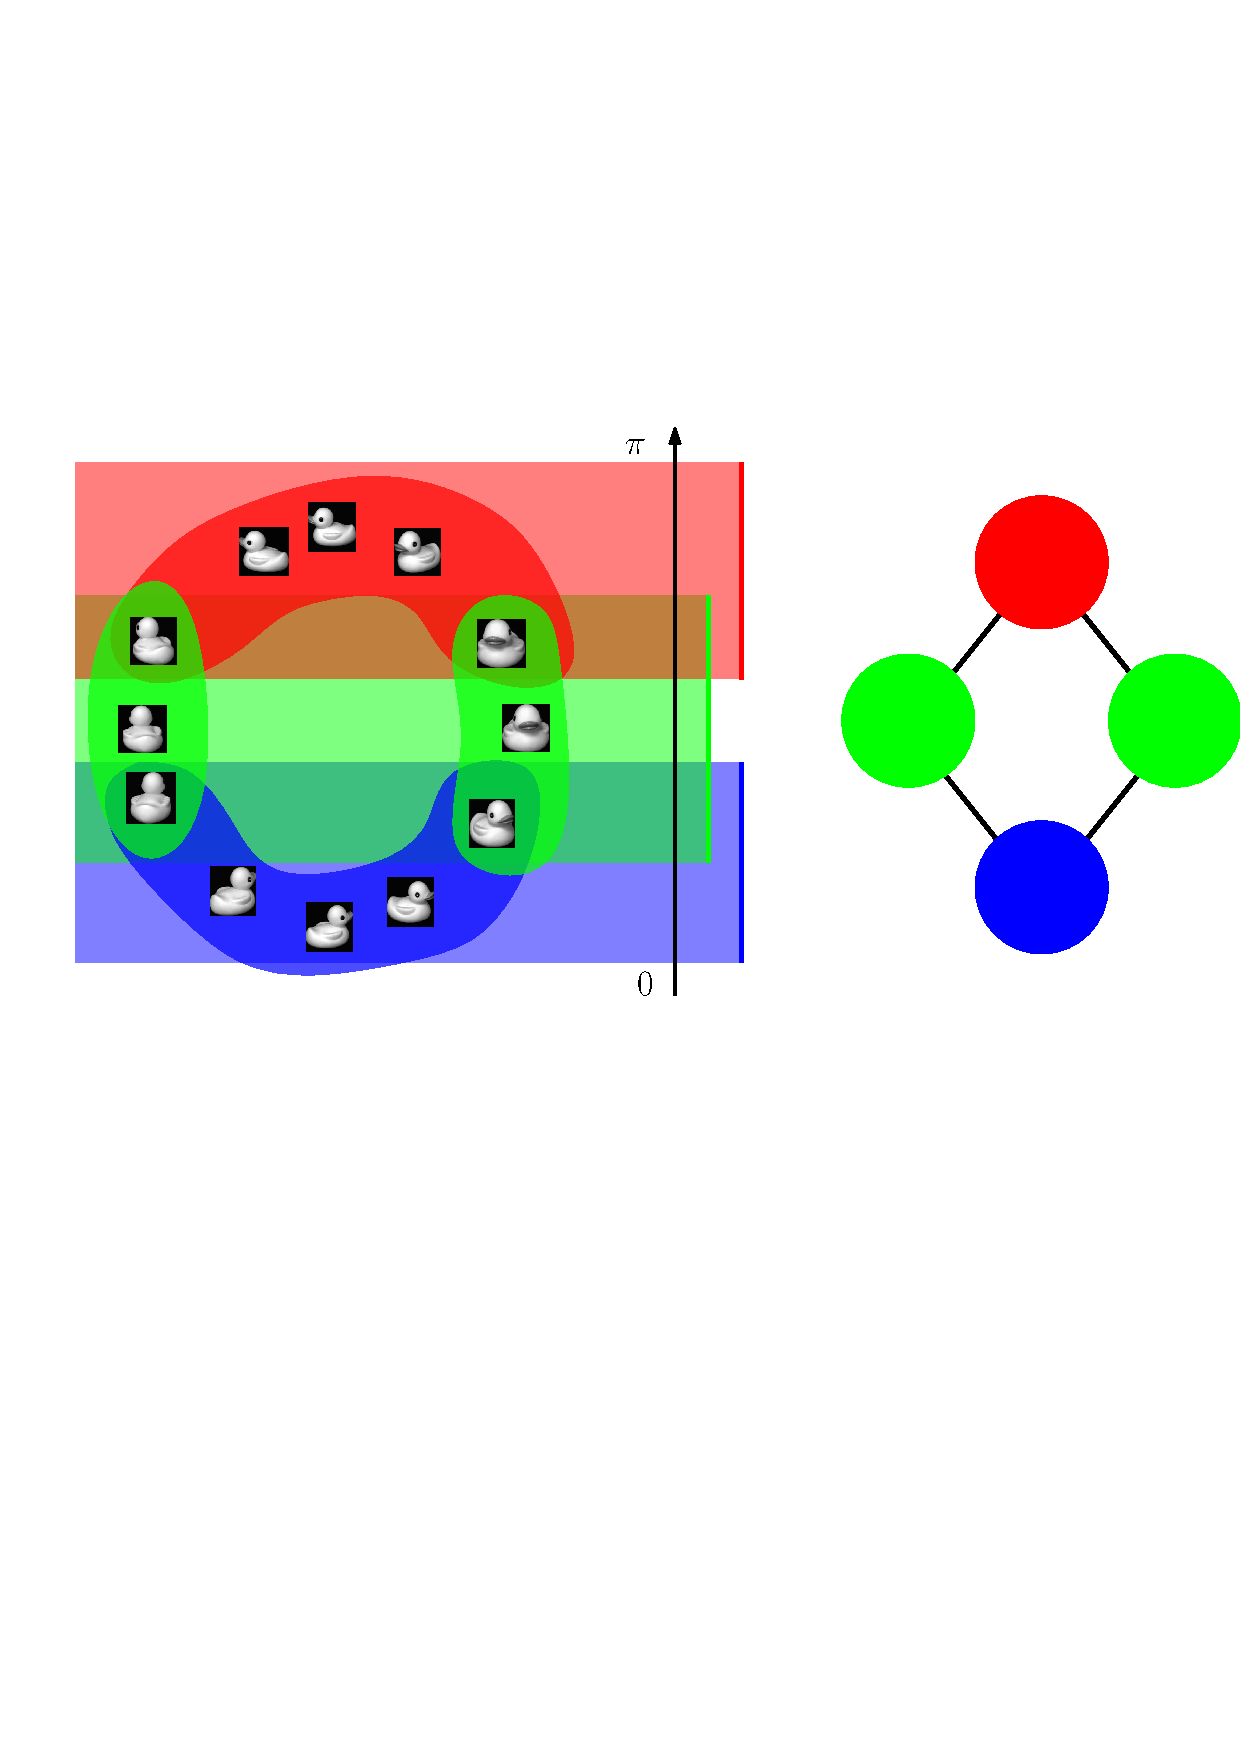
\includegraphics[width=.75\textwidth]{figures/ExampleMapper}
\caption[Mapper calcul\'e sur des images]{\label{fig:mapperima}
Exemple de Mapper calcul\'e sur le nuage d'images, avec la fonction d'angle et une couverture de trois intervalles.}
\end{figure}

%\begin{figure}[h]\centering
%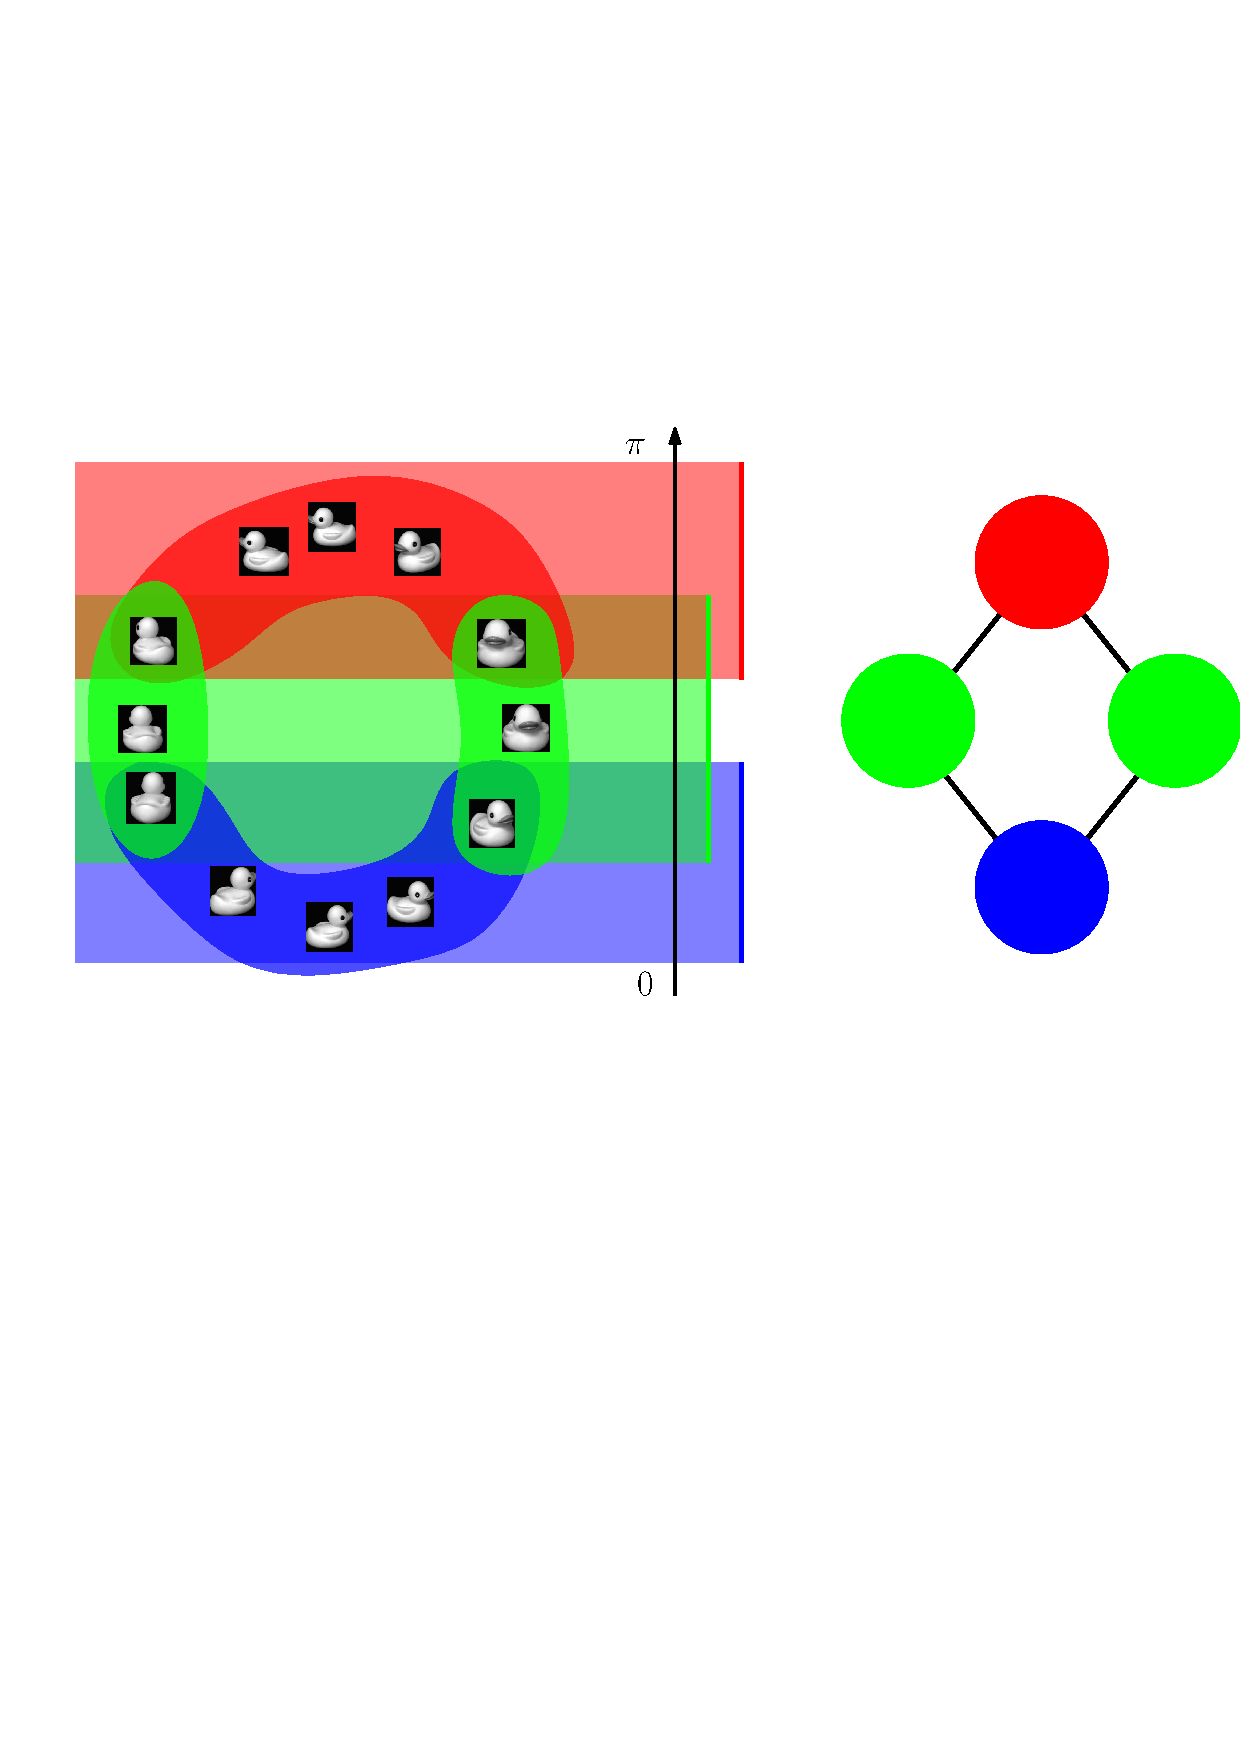
\includegraphics[width=.75\textwidth]{figures/ExampleMapper}
%\caption[Mapper on images]{\label{fig:mapper}Example of Mapper computed on the point cloud of images with the angle function and a cover of three intervals.}
%\end{figure}	

Nous fournissons un exemple dans la Figure~\ref{fig:mapperima}, o\`u nous consid\'erons de nouveau le nuage d'images. La fonction r\'eelle continue
est la valeur absolue de l'angle \`a partir duquel l'image a \'et\'e prise, et son image $[0,\pi]$ est couverte par trois intervalles (bleu, rouge et vert).
Dans les ant\'ec\'edents des intervalles rouge et bleu, il y a une seule composant connexe, tandis qu'il y en a deux dans l'ant\'ec\'edent de l'intervalle vert.
Le Mapper est obtenu en ajoutant des ar\`etes entre les composantes connexes, en fonction de la pr\'esence ou non de points de donn\'ees en commun \`a l'int\'erieur
de ces composantes; par exemple, les composantes connexes vertes et bleues, ou vertes et rouges, sont reli\'ees, mais pas celles qui sont rouges et bleues.
Le Mapper a l'homologie d'un cercle, est constitue une approximation directe du support sous-jacent au nuage d'images.

%We provide an example in Figure~\ref{fig:mapper}, where we consider again the point cloud of images. The continuous scalar-valued function is 
%the absolute value of the angle at which the picture was taken, and its image $[0,\pi]$ is covered with three intervals, the blue, green and red ones. 
%In the preimage of the red and blue intervals there is just one connected component, whereas there are two in the preimage of the green interval.
%We obtain the Mapper by putting edges between the connected components according to whether they share data points or not; for instance 
%green and blue or green and red connected components are linked whereas red and blue are not. The Mapper has the homology of the circle, and is a 
%direct approximation of the underlying support of the point cloud. 

Il est bon de remarquer que les longueurs des intervalles contr\^olent directement l'\'echelle \`a partir de laquelle on observe le nuage : si les
intervalles sont petits, le Mapper va avoir beaucoup de composantes d\'econnect\'ees puisque les ant\'ec\'edents contiendront au plus un point de donn\'ee.
A l'oppos\'e, si les intervalles sont larges, le Mapper aura peu de composantes puisque les ant\'ec\'edents vont contenir beaucoup de points de donn\'ees.

%Note that the lengths of the intervals in the cover directly control the scale at which data is observed: if the intervals are very small, the Mapper
%will have many disconnected nodes since the preimages of the intervals will contain at most one point. 
%On the opposite, if the intervals have large lengths,
%the Mapper will have only few nodes since the preimages of the intervals are going to contain many points.  

En pratique, le Mapper a deux domaines d'applications majeures. Le premier est la visualisation et le clustering.
En effet,  le Mapper fournit une visualisation des donn\'ees sous forme de graphe dont la topologie refl\`ete
celle des donn\'ees. Il apporte ainsi une information compl\'ementaire \`a celle des algorithmes de clustering usuels concernant
la structure interne des clusters 
%les sous-populations int\'eressantes des donn\'ees 
par l'identification de {\em branches} et de {\em boucles}
qui mettent en lumi\`ere des 
attributs topologiques
%sous-population 
potentiellement remarquables dans les groupes identifi\'es par clustering.
Voir par exemple~\cite{Yao09, Lum13, Sarikonda14, Hinks15} pour des exemples d'applications.
La deuxi\`eme application est la s\'election d'attributs. En effet, chaque attribut des donn\'ees peut \^etre \'evalu\'e
en regard de sa capacit\'e \`a diff\'erencier les 
attributs topologiques
%sous-populations int\'eressantes 
mentionn\'es plus haut (branches et boucles)
du reste des donn\'ees, via l'utilisation de tests statistiques, comme celui de Kolmogorov-Smirnov.
Voir par exemple~\cite{Lum13, Nielson15, Rucco15} pour des exemples d'applications.

%In practice, the Mapper has two major applications. The first one is data visualization and clustering.
%Indeed, the Mapper provides a visualization of the data in the form of a graph whose topology reflects
%that of the data. As such, it brings additional information to the usual clustering algorithms 
%about the interesting subpopulations of the data 
%by identifying {\em flares} and {\em loops} that outline potentially remarkable subpopulations
%in the various clusters. See e.g.~\cite{Yao09, Lum13, Sarikonda14, Hinks15} for examples of applications. 
%The second application of Mapper deals with feature selection. Indeed,
%each feature of the data can be evaluated on its ability to discriminate  
%the interesting subpopulations mentioned above (flares, loops) from the rest of the data, 
%using for instance Kolmogorov-Smirnov tests.
%See e.g.~\cite{Lum13, Nielson15, Rucco15} for examples of applications.   


\subsection{Principales limitations}

M\^eme si le Mapper et les diagrammes de persistance b\'en\'eficient de propri\'et\'es d\'esirables, plusieurs limitations
refr\`enent leur usage pratique, \`a savoir la {\em la difficult\'e de la s\'election de param\`etres pour Mapper}
%{\em manque de distance et de stabilit\'e pour le Mapper}
 et la {\em non lin\'earit\'e} de l'espace des diagrammes de persistance.

%\section{Main bottlenecks}

%Even though Mapper and persistence diagrams enjoy many desireable properties, several limitations
%slightly jeopardize their effective use in practice, namely the {\em lack of distance and stability results} for Mapper
%and the {\em non linearity} of the space of persistence diagrams. 



\paragraph*{Distance et stabilit\'e pour les Mappers et les graphes de Reeb}

%\paragraph*{Distances and stability for Mappers and Reeb graphs.}
%

Un probl\`eme du Mapper est que, contrairement aux diagrammes de persistance, il a un param\`etre, la couverture,
dont la s\'election \`a priori est difficile. A cause de cela, le Mapper appara\^it comme une construction tr\`es {\em instable} : 
il arrive que des Mappers calcul\'es sur des nuages de points similaires, comme dans la Figure~\ref{fig:instabiliteMapper},
ou avec des couvertures proches, comme dans la Figure~\ref{fig:instabilite}, soient tr\`es diff\'erents.

%One problem with the Mapper is that, contrary to the persistence diagrams, it has a parameter, which is the cover,
%and it is unclear how this cover should be tuned beforehand.
%Because of this, %arbitrary fixed cover, or scale,
%the Mapper seems to be a very {\em instable} construction:
%Indeed, a Mapper needs an arbitrary choice of cover, or scale, to be computed. Hence, 
%it may happen that Mappers computed on close point clouds, 
%as in Figure~\ref{fig:instabMapper}, or with similar covers, as in Figure~\ref{fig:instab},
%end up being very different.

\begin{figure}[h]\centering
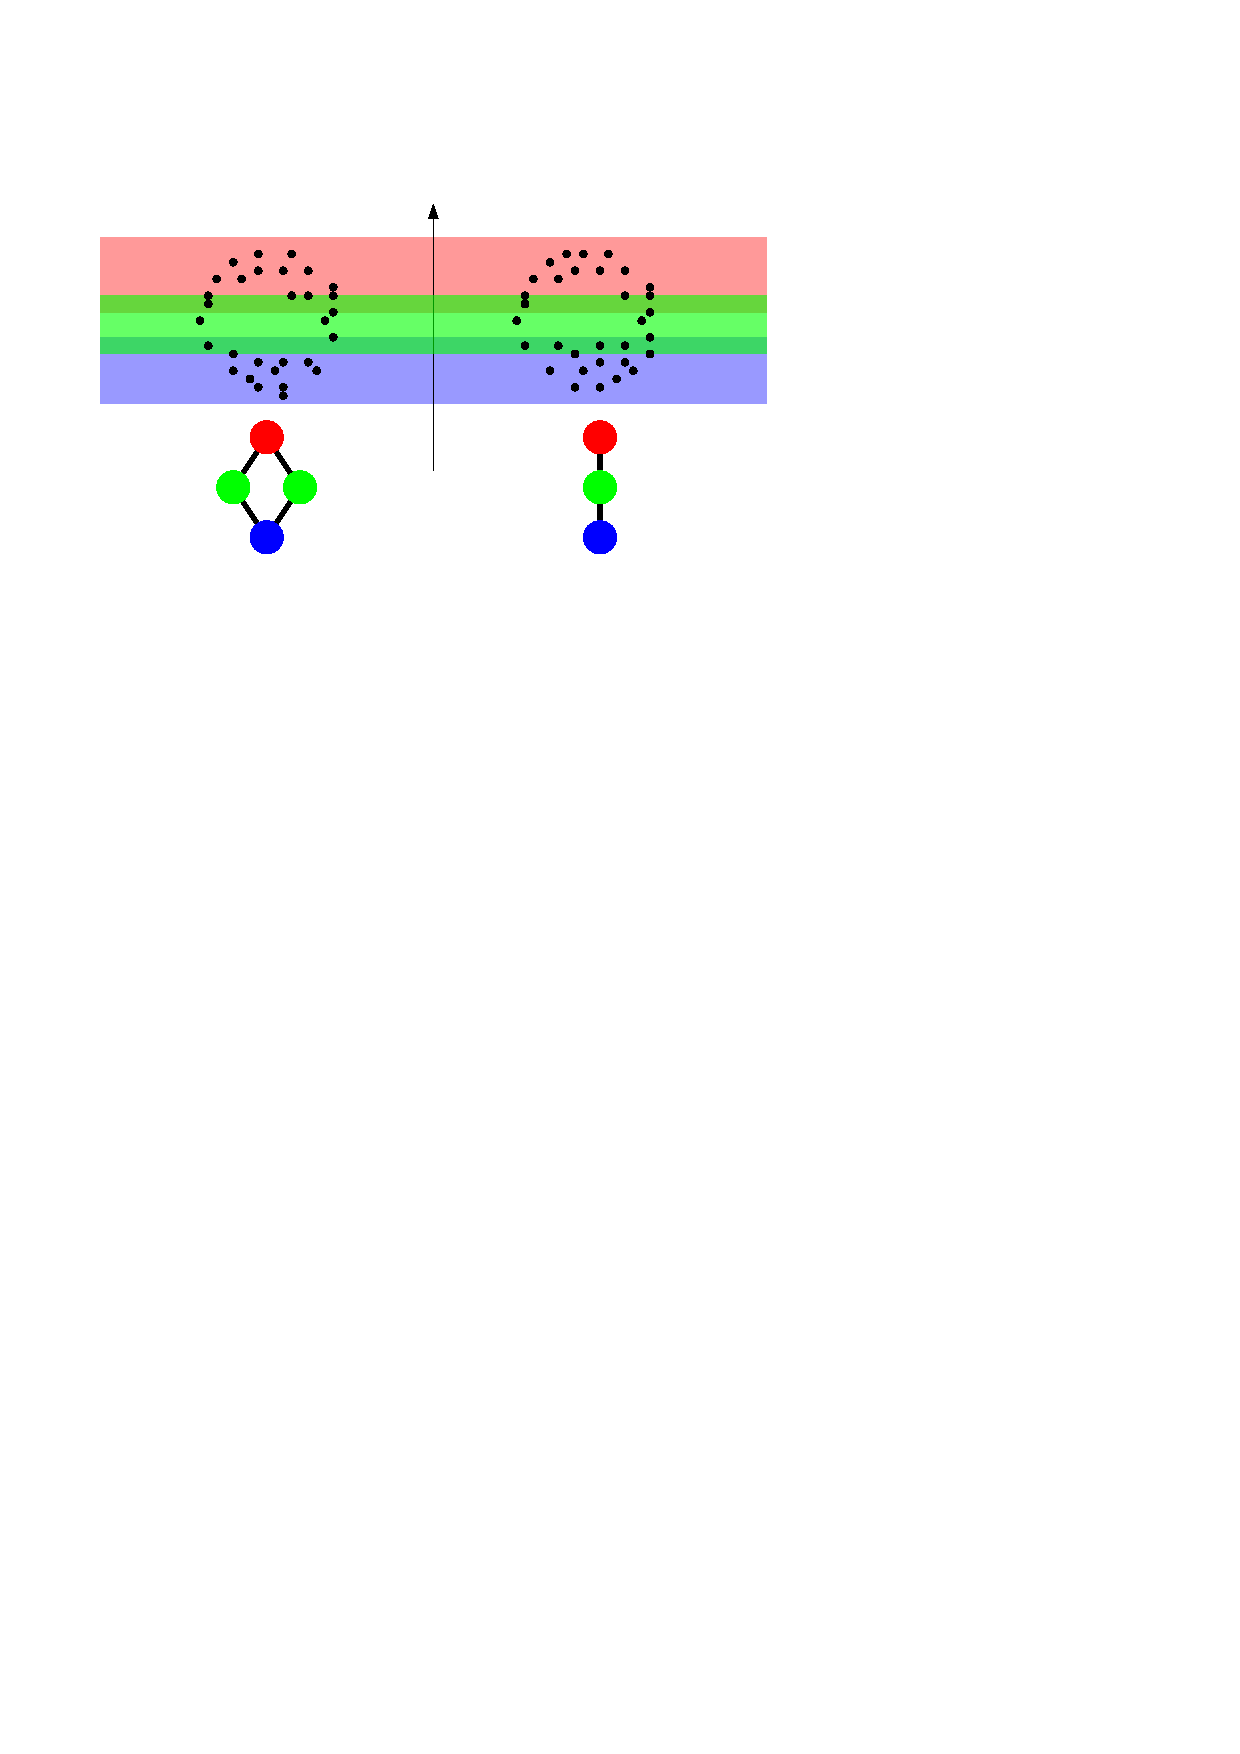
\includegraphics[width=10cm]{figures/ExampleInstabilityMapper}
\caption[Instabilit\'e de Mappers calcul\'es sur des espaces proches]{\label{fig:instabiliteMapper} 
Mappers calcul\'es sur des \'echantillonnages similaires du cercle, avec la fonction hauteur et une couverture  compos\'ee de trois intervalles.}
\end{figure}


%\begin{figure}[h]\centering
%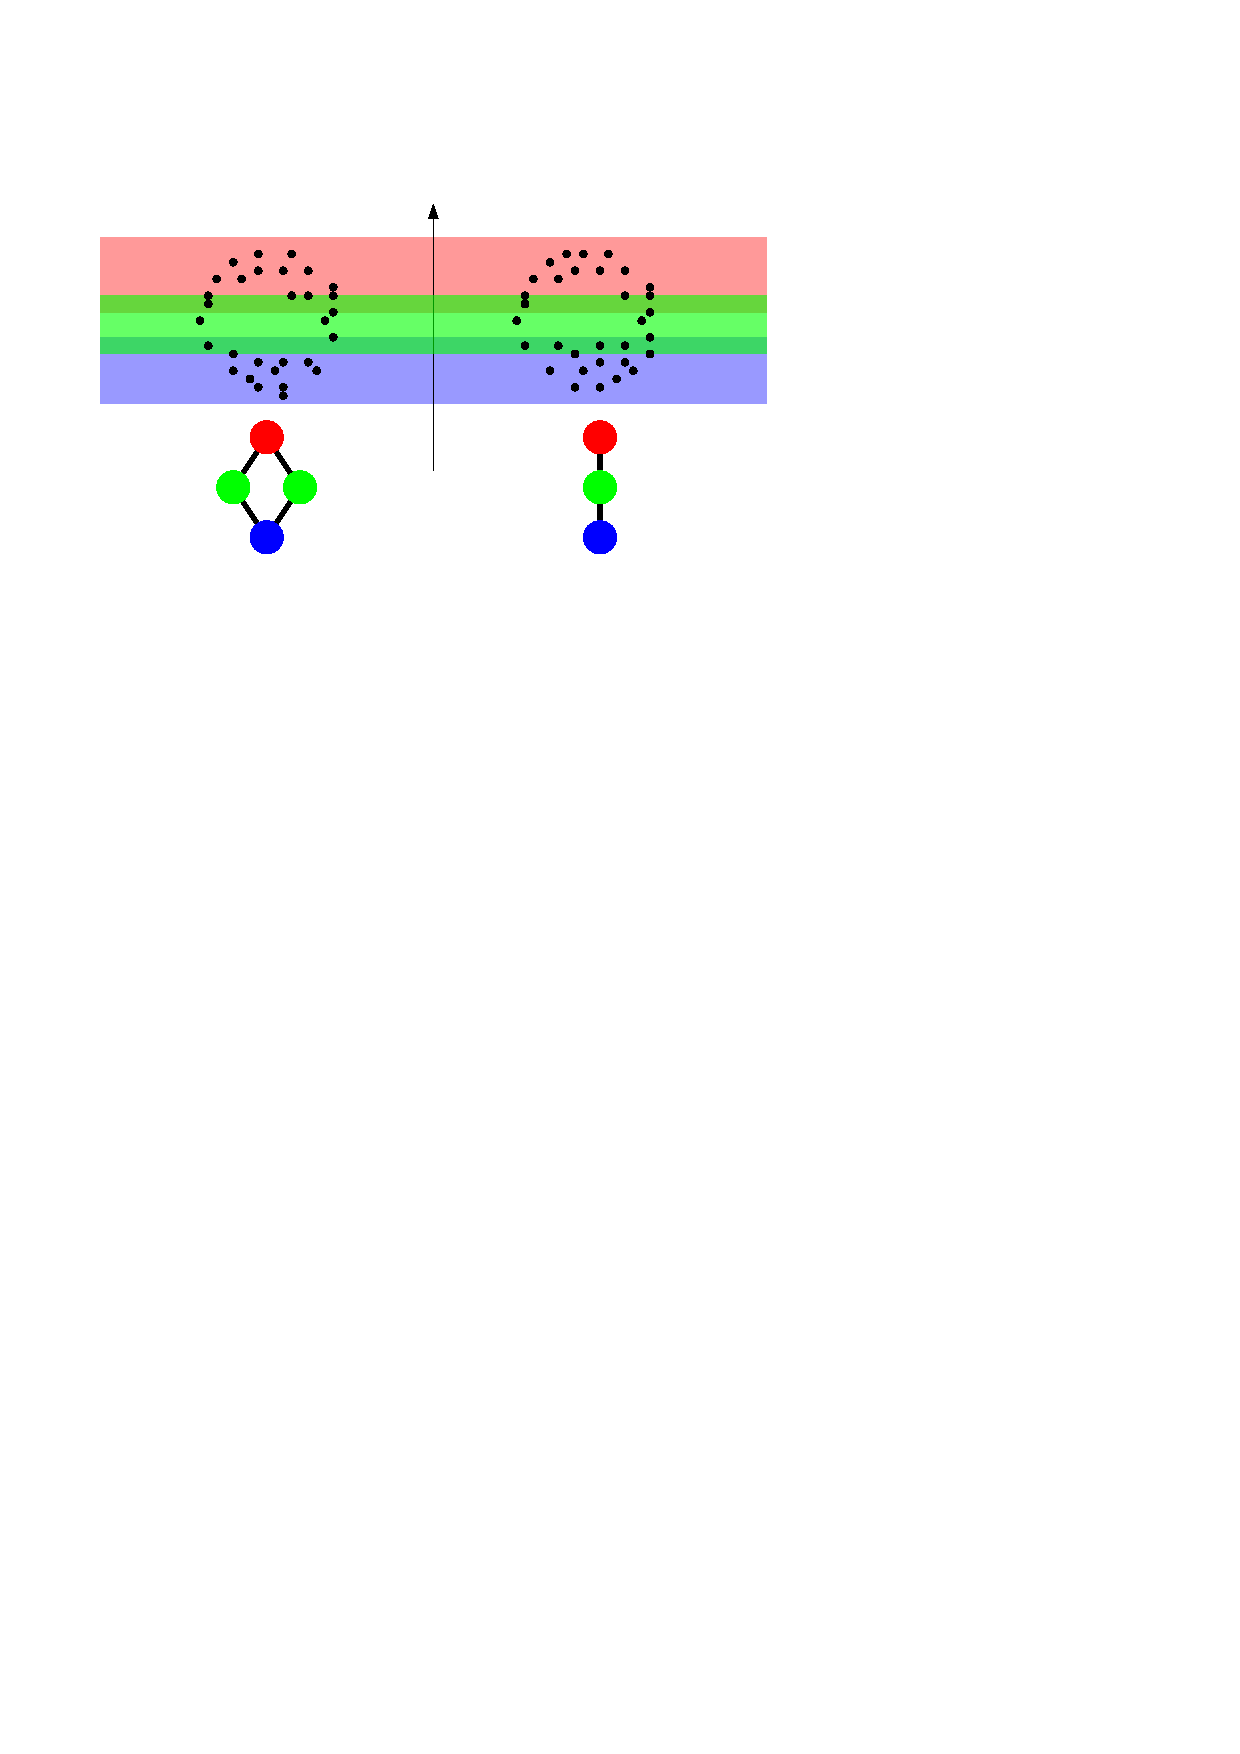
\includegraphics[width=10cm]{figures/ExampleInstabilityMapper}
%\caption[Instability of Mapper computed on close spaces]{\label{fig:instabMapper} Mappers of two similar samplings of the circle, computed with the height function
%and a cover with three intervals.}
%\end{figure}

Ce probl\`eme majeur est un obstacle important \`a son utilisation en exploration de donn\'ees.
La seule r\'eponse dans l'\'etat-de-l'art consiste \`a s\'electionner des param\`etres dans une grille de valeurs
pour lesquels le Mapper semble stable - voir~\cite{Nielson15} par exemple.

%This major drawback of Mapper is an important obstacle to its use  
%in exploratory data analysis with non trivial datasets. %We give another illustration of this phenomenon  on a dataset that we study further in Chapter~\ref{chap:MapperStatistic}. 
%The only answer proposed to 
%this drawback in the literature consists in selecting parameters in a range of values for which 
%the Mapper seems to be stable---see for instance~\cite{Nielson15}. 

\begin{figure}
\begin{tabular}{cc}
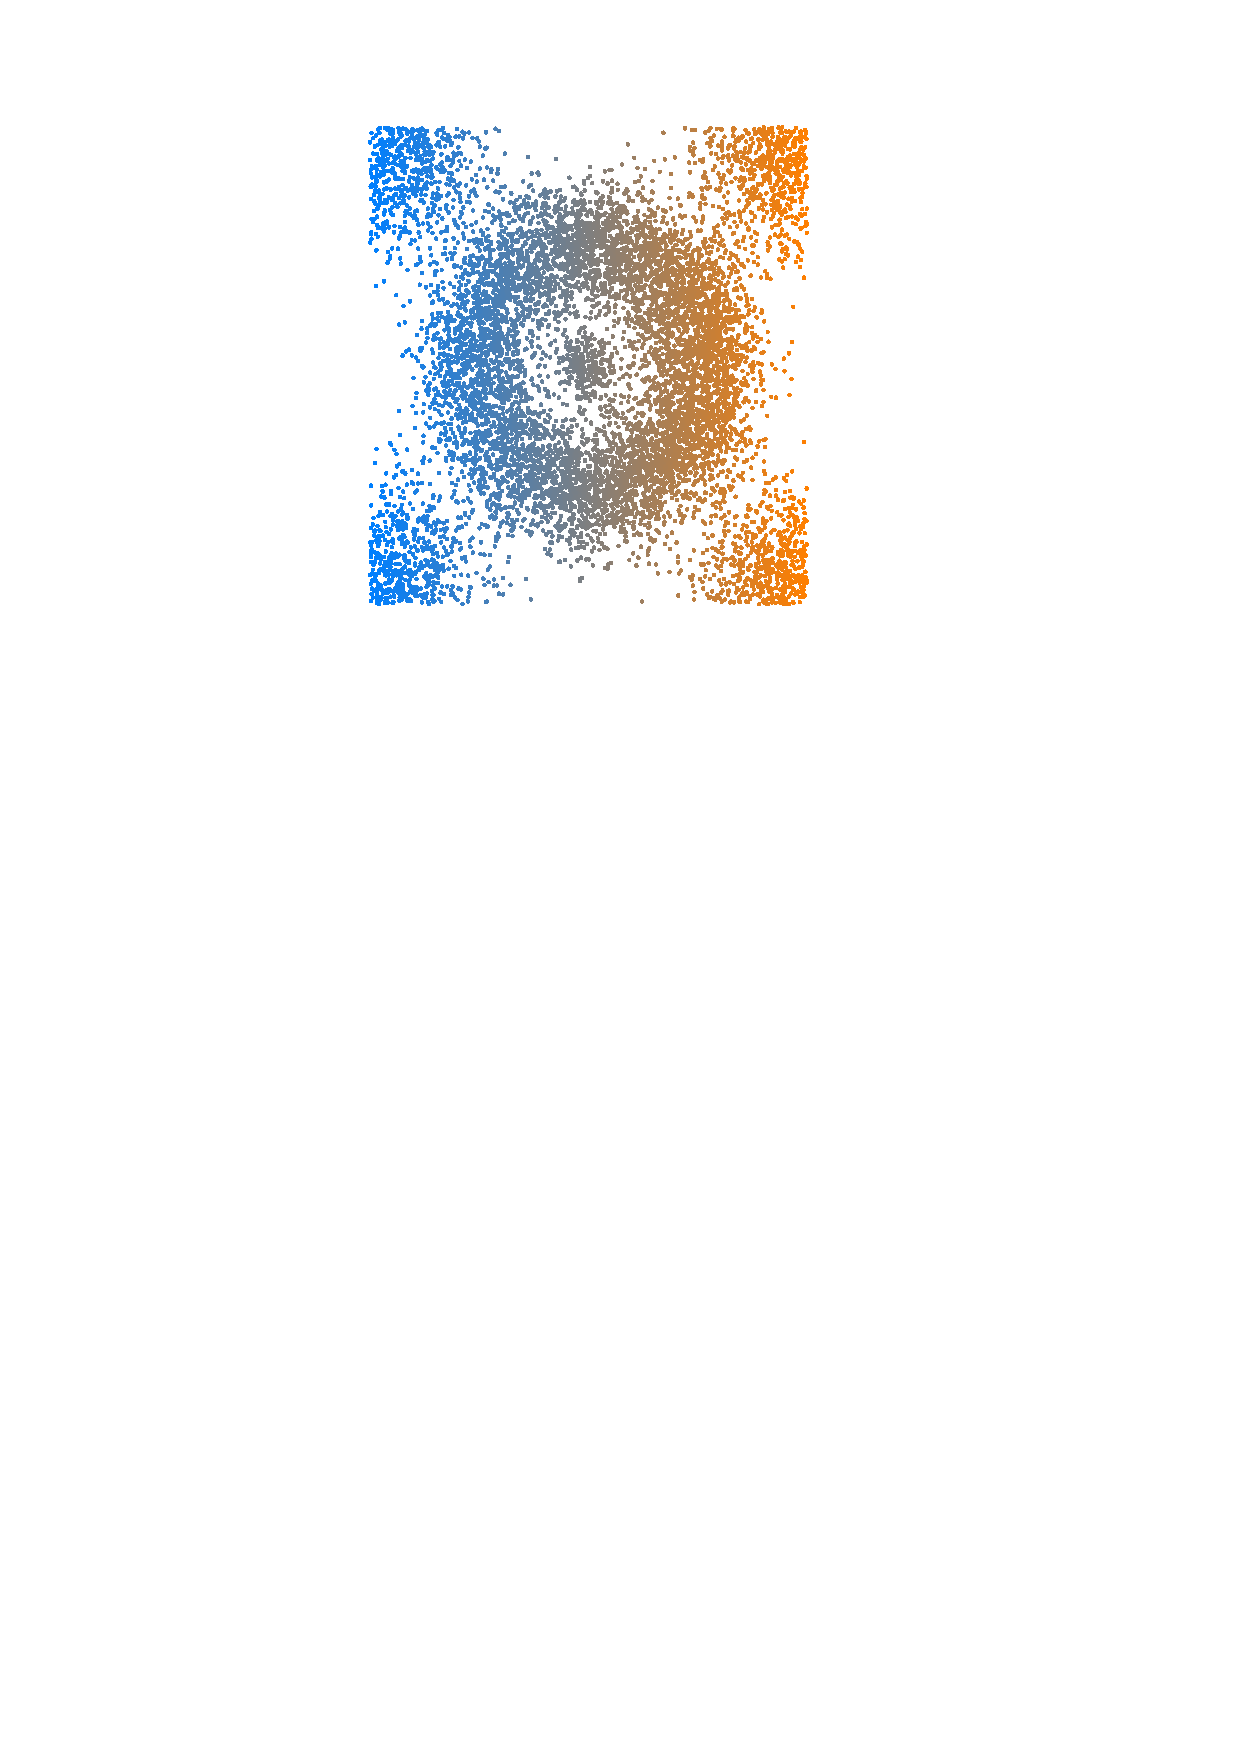
\includegraphics[width=6cm]{figures/crater_instab} & 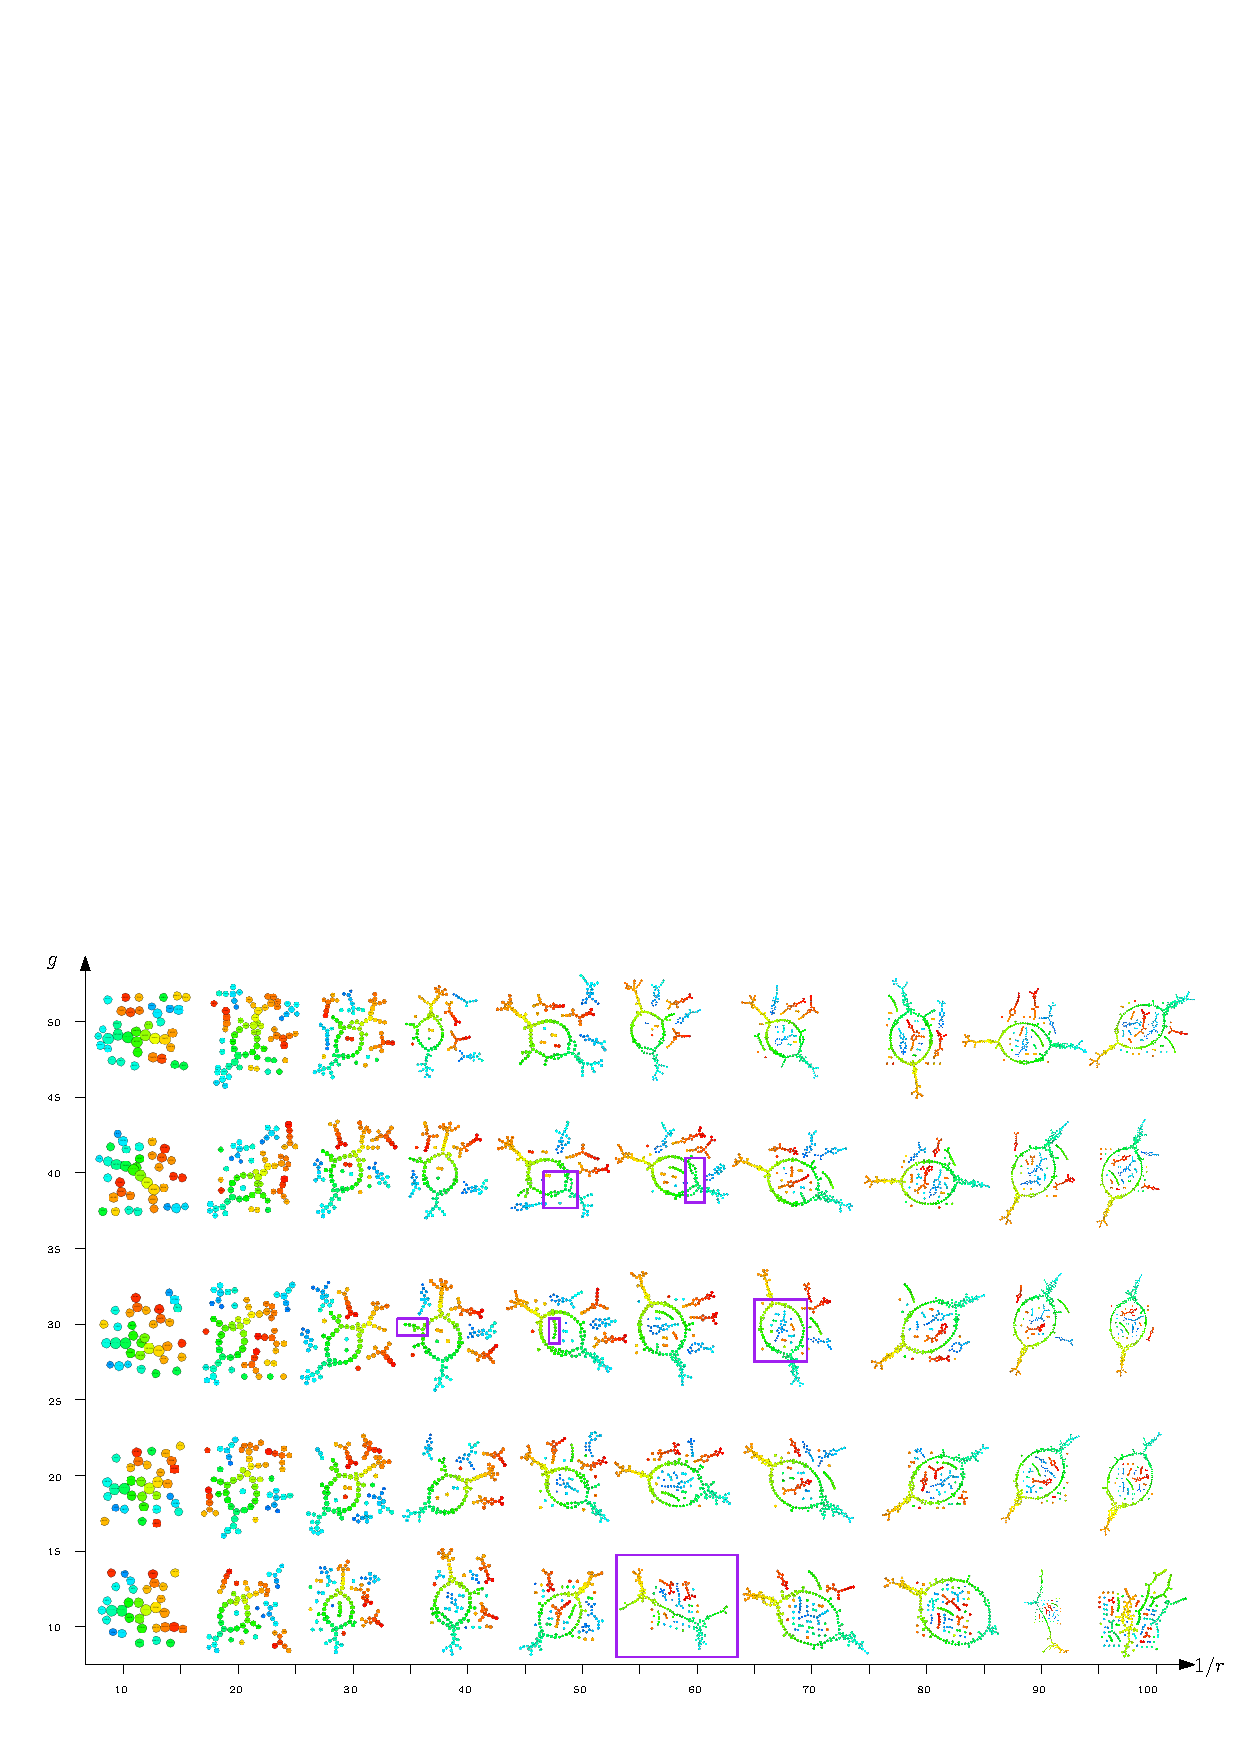
\includegraphics[width=10cm]{figures/instab}
\end{tabular}
\caption[Instabilit\'e de Mappers calcul\'es avec des couvertures proches ]{\label{fig:instabilite}
Un ensemble de Mappers calcul\'es sur le jeu de donn\'ees du crat\`ere avec des couvertures diff\'erentes ($r$ est la longueur des intervalles et $g$
est le pourcentage de chevauchement) et la coordonn\'ee horizontale. Gauche : jeu de donn\'ees du crat\`ere color\'e par les valeurs
de fonction, allant de bleu \`a orange. Droite : Mappers calcul\'es avec des param\`etres diff\'erents.
Les rectangles violets indiquent les attributs topologiques qui apparaissent ou disparaissent soudainement dans les Mappers.}
\end{figure}


%\begin{figure}
%\begin{tabular}{cc}
%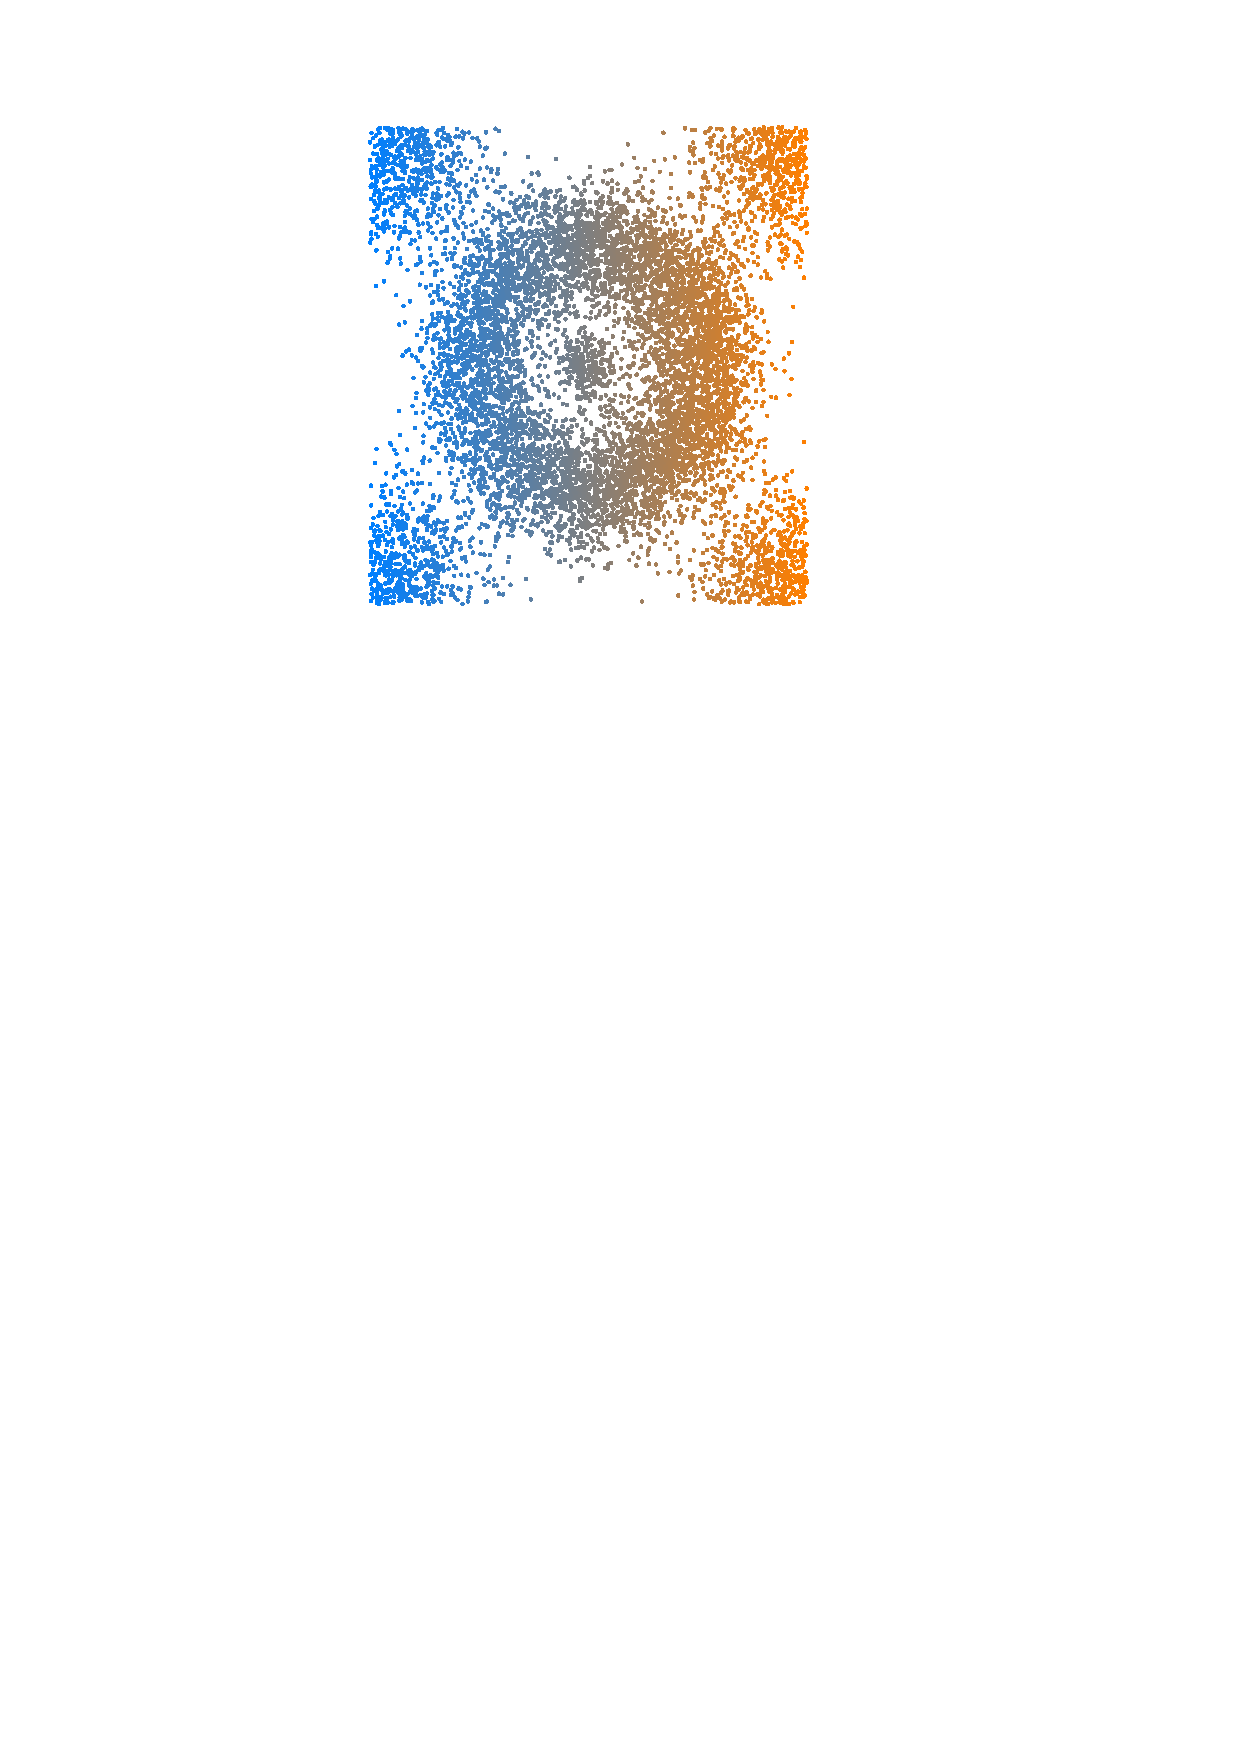
\includegraphics[width=6cm]{figures/crater_instab} & 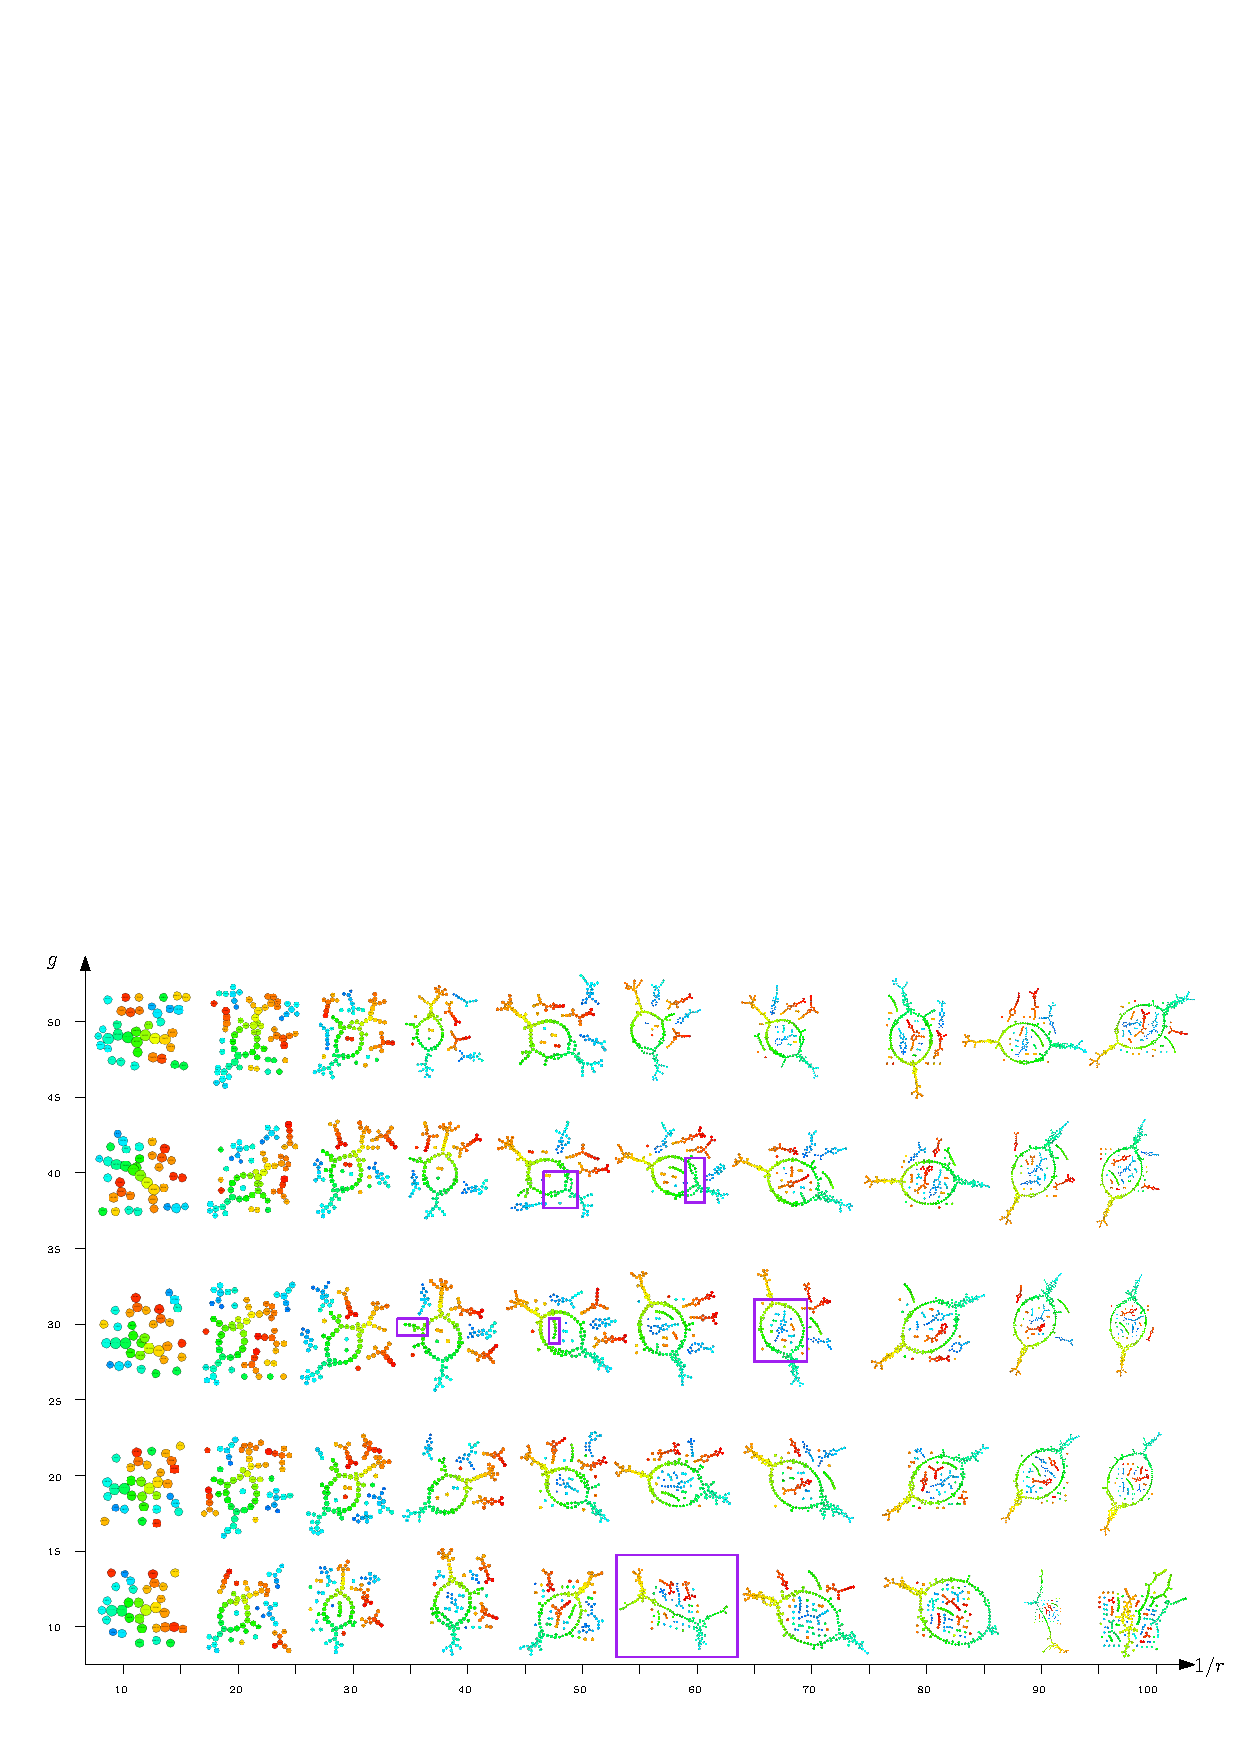
\includegraphics[width=10cm]{figures/instab}
%\end{tabular}
%\caption[Instability of Mapper computed with close covers]{\label{fig:instab}
%A collection of Mappers of the crater dataset computed with various covers ($r$ is the length of the intervals and $g$ is their overlap percentage)
%and the horizontal coordinate.
%Left: crater dataset colored with function values, from blue to orange. Right: outputs of Mapper with various parameters. 
%One can see that for some Mappers,
%The purple squares indicate topological features that suddenly appear and disappear in the Mappers. 
%These are discretization artifacts, that we overcome in this Chapter by appropriately tuning the parameters.
%}
%\end{figure}

Ainsi, prouver un r\'esultat de stabilit\'e pour les Mappers n\'ecessite de les comparer avec une distance qui d\'epend au moins de la couverture utilis\'ee.
Malheureusement, m\^eme si des distances th\'eoriques peuvent \^etre d\'efinies~\cite{Munch16}, 
la d\'efinition d'une distance calculable et interpr\'etable entre Mappers manque dans l'\'etat-de-l'art.
Pour g\'erer ce probl\`eme, on peut prendre inspiration d'une classe de descripteurs tr\`es semblables aux Mappers, les {\em graphes de Reeb}. 


%Hence, deriving a stability theorem for Mappers would require to compare them with a metric that depends at least on the cover. 
%Unfortunately, even the definition of a distance between Mappers is lacking in the literature. 
%To tackle this problem, one can take inspiration from another class of descriptors, which are very similar to Mapper, called the {\em Reeb graphs}.

\paragraph*{Graphes de Reeb.} M\^eme si les Mappers sont d\'efinis pour des nuages de points, leur extension \`a des espaces non discrets
est \'evidente, la diff\'erence \'etant que des techniques de clustering ne sont pas n\'ecessaires pour calculer les composantes connexes 
des ant\'ec\'edents puisqu'elles sont bien d\'efinies. Dans ce cas, faire tendre la longueur des intervalles vers z\'ero d\'efinit le {\em graphe de Reeb}.
%Il peut aussi \^etre d\'efini de mani\`ere \'equivalente comme l'espace quotient calcul\'e en identifiant tous les points appartenant \`a la m\^eme
%composante connexe d'un niveau de la fonction :  $f^{-1}(\alpha)$, o\`u $\alpha\in\R$.
Ainsi, les Mappers (calcul\'es sur des espaces non discrets) ne sont que des {\em approximations}, ou des {\em versions pixelis\'ees} des
graphes de Reeb, comme illustr\'e dans la Figure~\ref{fig:pixelizationM}.

%\paragraph*{Reeb graphs.} Note that the Mapper was originally defined for point clouds, but it can straightforwardly be extended to possibly
%non discrete topological spaces, for which clustering is not needed to compute the connected components of preimages.
%In that case, making the lengths of cover intervals go to zero leads to a limiting object called the {\em Reeb graph}.
%It can be equivalently defined as a quotient space computed by gluing together all
%points belonging to the same connected component of a level set of the filter: $f^{-1}(\alpha)$ where $\alpha\in\R$.
%Hence, Mappers (computed on non discrete topological spaces) are nothing but {\em approximations}, or 
%{\em pixelized versions} of Reeb graphs, as illustrated in Figure~\ref{fig:pixelization}.

\begin{figure}[h]\centering
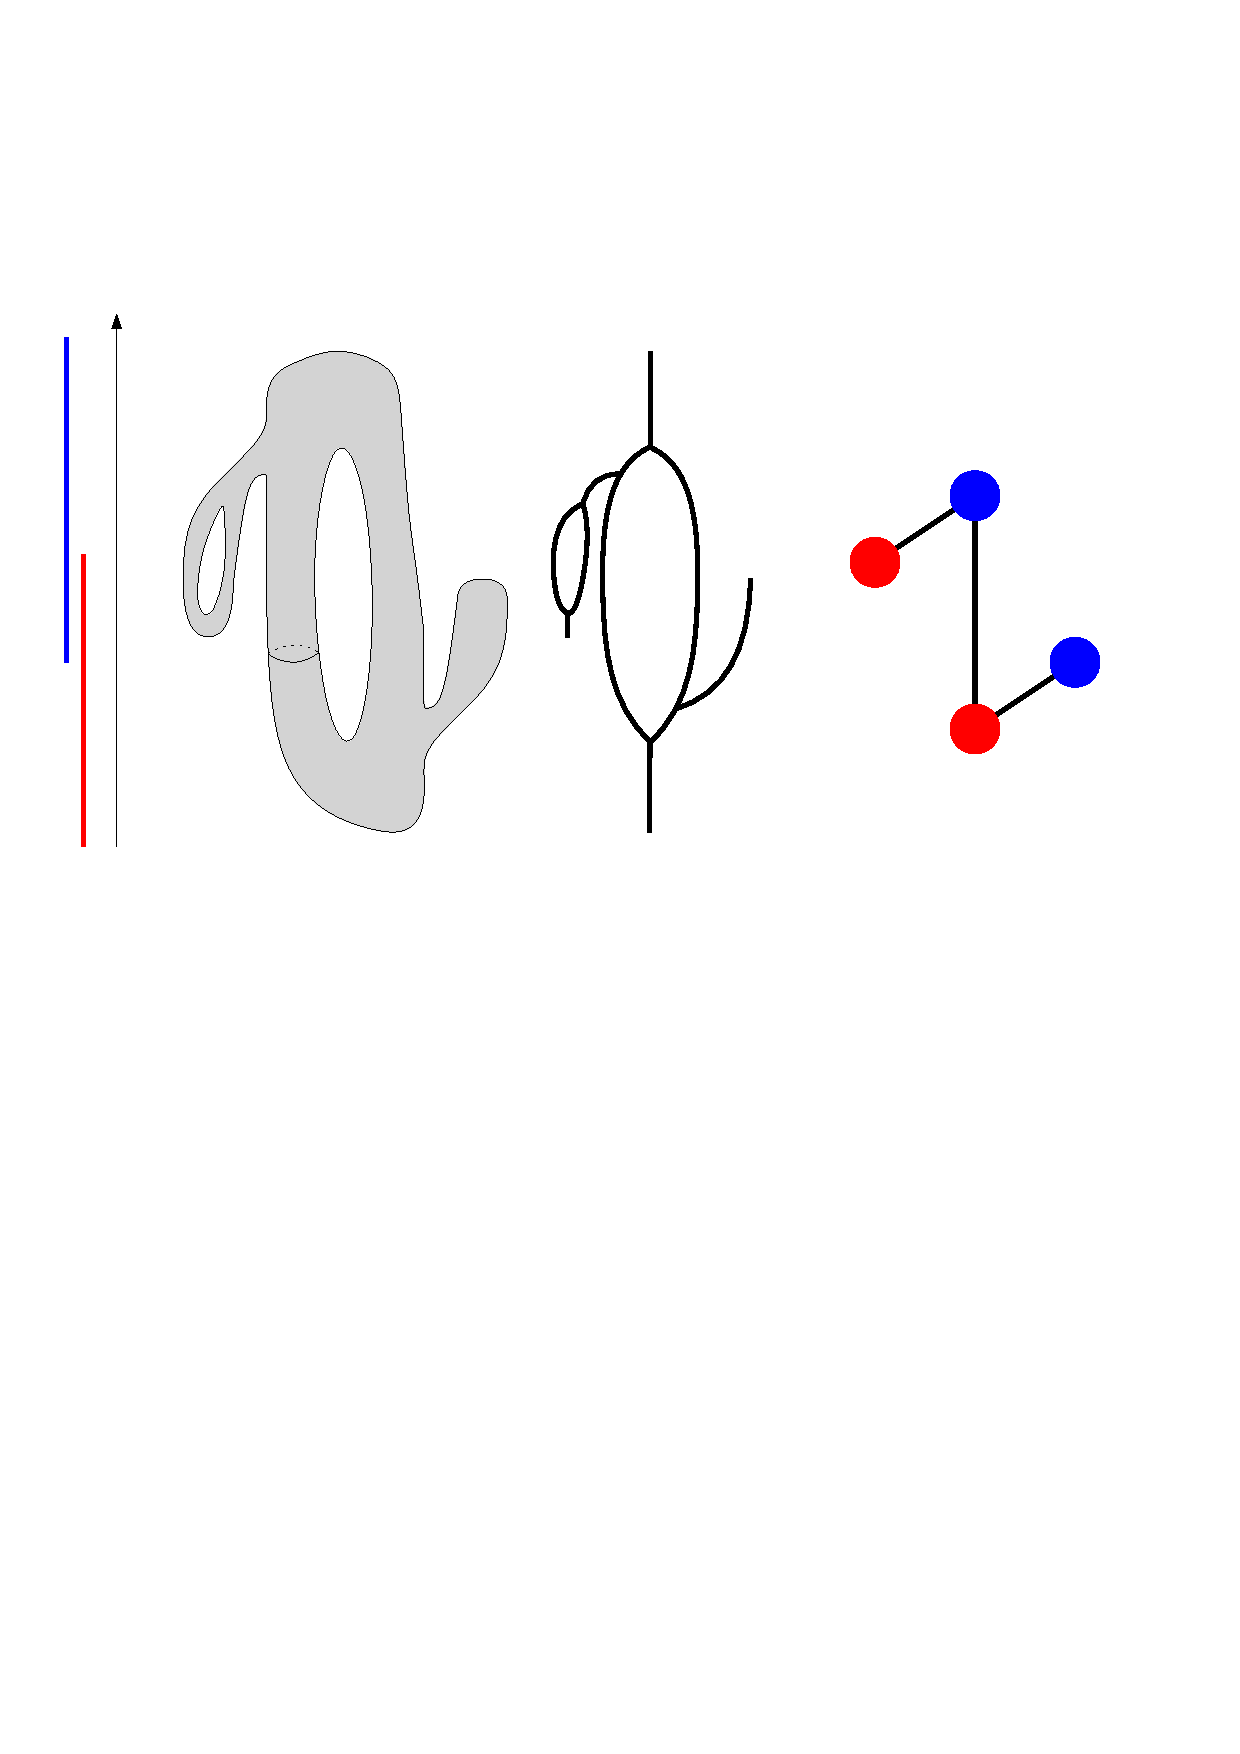
\includegraphics[width=10cm]{figures/ExamplePixelization}
\caption[Mapper vu comme une pixelisation du graphe de Reeb]{\label{fig:pixelizationM} 
Une surface plong\'ee dans $\R^3$ (gauche), son graphe de Reeb calcul\'e avec la fonction hauteur (milieu)
et son Mapper calcul\'e avec la fonction hauteur et une couverture \`a deux intervalles (droite).}
\end{figure}

%\begin{figure}[h]\centering
%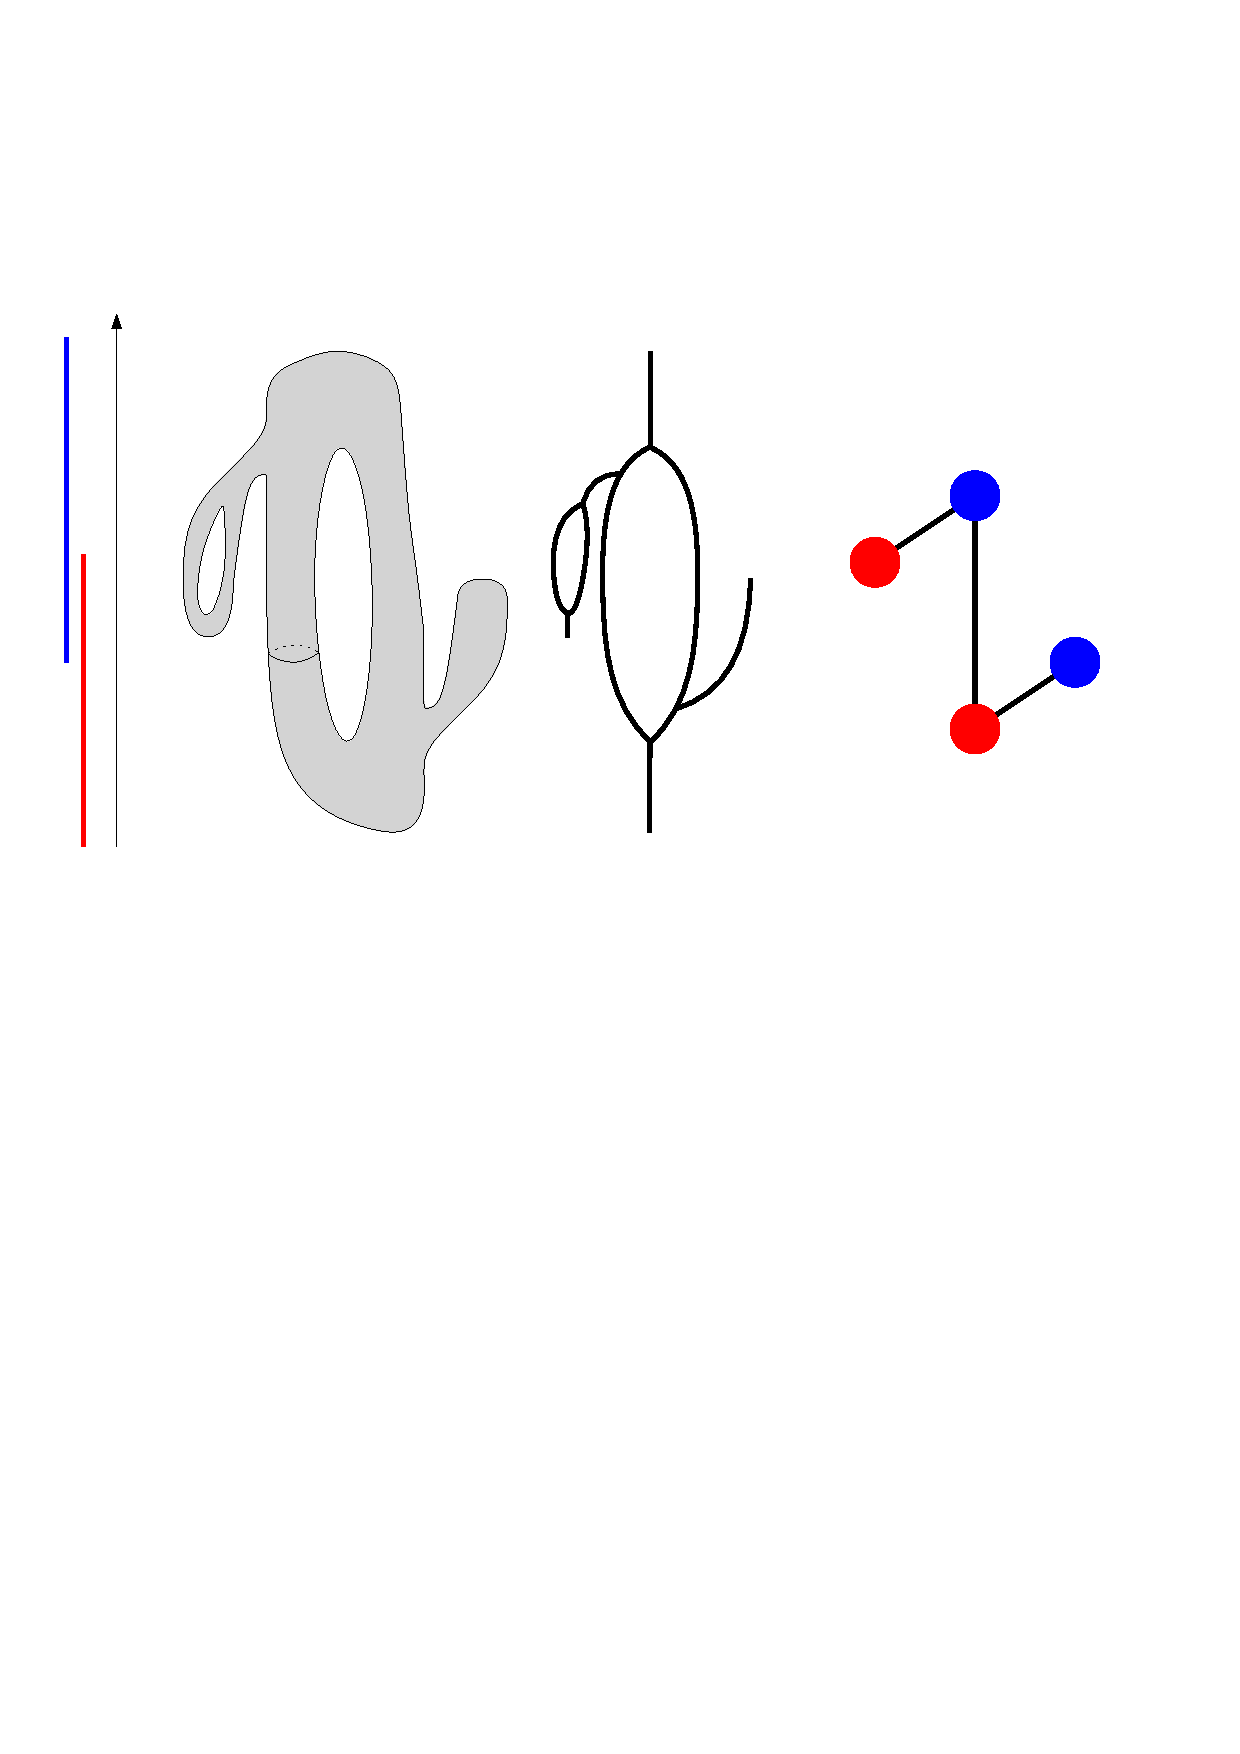
\includegraphics[width=10cm]{figures/ExamplePixelization}
%\caption[Mapper as a pixelization of the Reeb graph]{\label{fig:pixelization} A surface embedded in $\R^3$ (left), its Reeb graph computed with the height function (middle) and 
%its Mapper computed with the height function and a cover with two intervals (right).}
%end{figure}
  
Cette observation est cruciale car plusieurs distances, ainsi que des r\'esultats de stabilit\'e, ont \'et\'e obtenus 
pour les graphes de Reeb~\cite{Bauer16,Bauer14,deSilva16} et peuvent \^etre \'etendus aux Mappers.
Cependant, ces distances ne sont pas calculables et ne peuvent pas \^etre utilis\'ees en tant que telles en pratique~\cite{Agarwal15}.
La question de savoir s'il est possible de d\'efinir des distances stables et calculables pour les Mappers reste ainsi ouverte.

%This observation is important since several natural metrics enjoying stability theorems already exist for Reeb graphs~\cite{Bauer16,Bauer14,deSilva16}
%and can be extended for Mappers. 
%However, these metrics are not computable and thus cannot be used as is in practice~\cite{Agarwal15}. Hence, there is an open question about how
%to define metrics for Mappers which would be both computable and stable.


  
%from the continuous
%\footnote{By continuous, we mean computable on possibly non discrete topological spaces.} counterpart of Mapper, 
%called the {\em Reeb graph}: the Reeb graph of a topological space is computed by   It can be 
%seen as a Mapper computed with open intervals whose length is infinitely small. 
%Alternatively, the Mapper can be seen as a {\em pixelized} version of the Reeb graph. 
%The problem is that of the distance used to compare Mappers. Indeed, it is unclear how to properly measure the similarity of Mappers. 
%In order to obtain a stability result similar to that of persistence diagrams,
%a suitable distance should depend on the cover used to compute the Mappers. 

\paragraph*{Non lin\'earit\'e de l'espace des diagrammes de persistance.}

M\^eme si les diagrammes de persistance sont stables, ils ne peuvent pas \^etre utilis\'es syst\'ematiquement par des algorithmes
d'apprentissage automatique. En effet, une classe tr\`es large de ces algorithmes n\'ecessitent que les donn\'ees soient soit des vecteurs
d'un espace Euclidien (comme les for\^ets al\'eatoires), ou d'un espace de Hilbert (comme les SVM).
L'espace des diagrammes de persistance, \'equip\'e avec la distance bottleneck, n'est malheureusement ni l'un ni l'autre.
M\^eme les moyennes de Fr\'echet ne sont pas bien d\'efinies~\cite{Turner14}. 
L'{\em astuce du noyau} permet cependant de traiter ce genre de donn\'ees.
En supposant que les points de donn\'ees vivent dans un espace m\'etrique $(X,d_X)$, l'astuce du noyau n\'ecessite seulement 
une fonction semi-d\'efinie positive, appel\'ee {\em noyau}, c'est-\`a-dire une fonction $k:X\times X\rightarrow\R$ telle que, pour tous 
$a_1,\cdots,a_n\in\R$ et  $x_1,\cdots,x_n\in X$, on ait :
$$\sum_{i,j}a_ia_jk(x_i,x_j)\geq 0.$$ 
Gr\`ace au th\'eor\^eme de Moore-Aronszajn~\cite{Aronszajn50}, les valeurs du  noyau calcul\'ees sur des points de donn\'ees peuvent \^etre d\'emontr\'ees
\'egales \`a l'\'evaluation d'un produit scalaire entre les images des points de donn\'ees par un plongement dans un espace de Hilbert sp\'ecifique
qui d\'epend uniquement de $k$ et qui est en g\'en\'eral inconnu.
Plus formellement, il existe un espace de Hilbert $\mathcal H_k$ tel que, pour tous $x,y\in X$, on ait : 
$$k(x,y)=\langle\Phi_k(x),\Phi_k(y)\rangle_{\mathcal H_k},$$
pour un certain plongement $\Phi_k$.
Les valeurs du noyau peuvent donc \^etre consid\'er\'ees comme des produits scalaires g\'en\'eralis\'es entre les points de donn\'ees, et peuvent \^etre
directement utilis\'es par les algorithmes d'apprentissage.
Dans le cas qui nous int\'eresse, la question est ainsi de trouver de tels noyaux pour les diagrammes de persistance.



%\paragraph*{Non linearity of persistence diagrams.}
%
%Even though persistence diagrams are stable descriptors, they cannot be plugged directly into Machine Learning algorithms.
%Indeed, most of these algorithms require the data to lie either in Euclidean space (such as random forests), 
%or at least in a Hilbert space (such as SVM).
%However, the space of persistence diagrams, equipped with the bottleneck distance, is neither Euclidean nor Hilbert.
%Even Fr\'echet means are not well-defined~\cite{Turner14}. Fortunately,
%the {\em kernel trick} allows to handle this kind of data.
%Assuming data points lie in metric space $(X,d_X)$, the kernel trick only requires a positive semi-definite function,  
%called a {\em kernel}, i.e. a function $k:X\times X\rightarrow\R$ such that, for any $a_1,\cdots,a_n\in\R$ and $x_1,\cdots,x_n\in X$:
%$$\sum_{i,j}a_ia_jk(x_i,x_j)\geq 0.$$ 
%Due to Moore-Aronszajn's theorem~\cite{Aronszajn50}, kernel values can be proven equal to the evaluation
%of the scalar product between embeddings of data into a specific Hilbert space that depends only on $k$ and is generally unknown. 
%More formally, there exists a Hilbert space $\mathcal H_k$ such that, for any $x,y\in X$: 
%$$k(x,y)=\langle\Phi_k(x),\Phi_k(y)\rangle_{\mathcal H_k},$$
%where the embedding $\Phi_k$ is called the {\em feature map} of $k$.
%Kernel values can thus be seen as generalized scalar products between data points, and can be directly plugged into Machine Learning algorithms. 
%Hence, in our case, the question becomes that of finding kernels for persistence diagrams.

Une mani\`ere standard de proc\'eder pour d\'efinir un noyau pour des points d'un espace m\'etrique $(X,d_X)$
est d'utiliser des fonctions {\em Gaussiennes} : 
$$k_\sigma(x,y)={\rm exp}\left(-\frac{d_X(x,y)}{2\sigma^2}\right),$$
o\`u $\sigma>0$ est un param\`etre d'\'echelle. Un th\'eor\^eme de Berg et al.~\cite{Berg84} stipule que  
$k_\sigma$ est un noyau, c'est-\`a-dire une fonction semi-d\'efinie positive, pour tous  $\sigma>0$
si et seulement si $d_X$ est {\em conditionnellement semi-d\'efinite n\'egative}, c'est-\`a-dire est telle qu'on ait 
$\sum_{i,j}a_ia_jd_X(x_i,x_j)\leq 0$ pour tous $x_1,\cdots,x_n\in X$ et $a_1,\cdots,a_n\in\R$ tels que $\sum_{i=1}^n a_i=0$.
Malheureusement, comme montr\'e par Reininghaus et al.~\cite{Reininghaus14}, %ont montr\'e que 
la distance bottleneck $\distb$ pour les diagrammes de persistance n'est pas conditionnellement semi-d\'efinite n\'egative. Il est m\^eme possible de trouver
des contre-exemples pour les distances de Wasserstein,
une autre classe de distance pour diagrammes. L'utilisation de noyaux Gaussiens pour les diagrammes de persistance est donc impossible
avec leurs m\'etriques canoniques. 

%A common way to define kernels for points lying in a metric space $(X,d_X)$ is to use {\em Gaussian} functions:
%$$k_\sigma(x,y)={\rm exp}\left(-\frac{d_X(x,y)}{2\sigma^2}\right),$$
%where $\sigma >0$ is a bandwidth parameter. A theorem of Berg et al.~\cite{Berg84} shows that $k_\sigma$ is a kernel, i.e. positive semi-definite, for all $\sigma>0$
%if and only if $d_X$ is {\em negative semi-definite}, meaning that  $\sum_{i,j}a_ia_jd_X(x_i,x_j)\leq 0$, for any $x_1,\cdots,x_n\in X$ and $a_1,\cdots,a_n\in\R$
%such that $\sum_{i=1}^n a_i=0$. Unfortunately, Reininghaus et al.~\cite{Reininghaus14} have shown that the bottleneck distance $\distb$ for persistence diagrams
% is not negative semi-definite. Actually, one can build
%counter examples even for Wasserstein distances, which is another widely used class of distances.
%Hence, the use of Gaussian-type kernels for persistence diagrams is not possible with their canonical metrics.   

N\'eanmoins, plusieurs noyaux ont \'et\'e propos\'es au cours des derni\`eres ann\'ees~\cite{Adams17,Bubenik15,Kusano16,Reininghaus15}, 
b\'en\'eficiant tous de r\'esultats de stabilit\'e bornant sup\'erieurement la distance entre les plongements des diagrammes par les distances
bottleneck ou de Wasserstein entre les diagrammes eux-m\^emes. En d'autres termes, la distorsion m\'etrique 
$${\rm dist}(\dg,\dg')=\frac{\|\Phi_k(\dg)-\Phi_k(\dg')\|_{\mathcal H_k}}{\distb(\dg,\dg')}$$
est born\'ee sup\'erieurement.
Cependant, le calcul d'une borne inf\'erieure non triviale reste ouvert : il se pourrait que les plongements de diagrammes diff\'erents soient 
en fait tr\`es proches l'un de l'autre, ce qui n'est pas d\'esirable en pratique pour la discriminativit\'e d'un noyau.
Par exemple, le plongement constant, qui envoie tous les diagrammes sur un m\^eme point d'un espace de Hilbert sp\'ecifique,
est stable (les distances entre images dans l'espace de Hilbert \'etant toujours nulles), mais les 
r\'esultats du noyau correspondant seront \'evidemment tr\`es faibles.   
Plus g\'en\'eralement, le comportement et les propri\'et\'es des distances dans les espaces de Hilbert induits par des noyaux sont flous,
et la question de savoir s'il existe des noyaux avec des propri\'et\'es th\'eoriques de discriminativit\'e est ouverte. 

%Nevertheless, several kernels for persistence diagrams have been proposed in the last few years~\cite{Adams17,Bubenik15,Kusano16,Reininghaus15}, 
%all of them enjoying stability theorems upper bounding the distance
%between the embeddings of the persistence diagrams by the bottleneck or the Wasserstein distances between them. 
%Hence, the metric distortion $${\rm dist}(\dg,\dg')=\frac{\|\Phi_k(\dg)-\Phi_k(\dg')\|_{\mathcal H_k}}{\distb(\dg,\dg')}$$
%is in general upper bounded. However, it is unclear whether it is also lower bounded or not: it may happen that the embeddings
%of very different persistence diagrams actually lie very close to each other, which is not desireable as for the discriminative power of the kernel.
%Think for instance of a constant kernel embedding: all persistence diagrams are mapped to the same element of a specific Hilbert space. 
%These embeddings are stable since their pairwise distances are all zero, but of course the kernel's results are very poor when 
%plugged into Machine Learning algorithms.  
%More generally, little is known concerning the behaviour and the properties of metrics of Hilbert spaces induced by kernels for persistence diagrams,
%and it remains an open question whether theoretical results on discriminative power of kernels can be stated and proved or not.     

\subsection{Contributions}


%\section{Contributions}


Dans cette th\`ese, nous nous penchons sur trois probl\`emes : 
l'interpr\'etation des attributs topologiques) du Mapper (par exemple avec des r\'egions de confiance), le r\'eglage de ses param\`etres, et
l'int\'egration globale des descripteurs topologiques en apprentissage automatique. 
%nous proposons des r\'eponses aux limitations des graphes de Reeb, Mappers et diagrammes de persistance soulev\'ees plus haut.

%In this thesis, we investigate and propose answers to the limitations of Reeb graphs, Mapper and persistence diagrams that we mentioned before. 

\paragraph*{Distance entre graphes de Reeb.} Dans le Chapitre~\ref{chap:backgroundTelescopesReeb}, nous d\'efinissons une pseudodistance calculable
entre graphes de Reeb, qui revient \`a comparer leurs diagrammes de persistance.
Nous montrons aussi que cette pseudodistance est en fait {\em localement \'equivalente} aux autres distances existantes pour les graphes de Reeb.
Cette \'equivalence locale est alors utilis\'ee pour \'etudier les propri\'et\'es de l'espace m\'etrique des graphes de Reeb, 
\'equip\'e des distances {\em intrins\`eques}.
Nous montrons que toutes ces distances intrins\`eques sont {\em fortement \'equivalentes}, ce qui nous permet d'englober toutes les techniques
pour comparer des graphes de Reeb en une seule approche. Ce travail a \'et\'e publi\'e dans les proceedings du Symposium on 
Computational Geometry 2017~\cite{Carriere17a}.   

%\paragraph*{Distance between Reeb graphs.} 
%In Chapter~\ref{chap:backgroundTelescopesReeb}, we define a computable pseudometric between Reeb graphs
%by comparing their persistence diagrams.
%We recall that, as explained before, all proposed metrics so far for Reeb graphs 
%are intractable. Hence, our first contribution is to  
%Even though this distance is only a pseudometric, we are able to show
%that it is {\em locally equivalent} to other metrics. This local equivalence is then used to study metric properties of the space of Reeb graphs
%equipped with {\em intrinsic metrics}: we prove that all such intrinsic metrics are {\em strongly equivalent}, thus encompassing 
%all approaches to compare Reeb graphs into a single framework. This work has been published~\cite{Carriere17a}. 

\paragraph*{Structure du Mapper.} Dans le Chapitre~\ref{chap:MapperStability}, nous fournissons un lien entre les diagrammes de persistance
du graphe de Reeb et ceux du Mapper (calcul\'e sur le m\^eme espace topologique).
Plus sp\'ecifiquement, nous montrons que le diagramme de persistance du Mapper est obtenu \`a partir de celui du graphe de Reeb en supprimant 
des points sp\'ecifiques, \`a savoir ceux qui appartiennent \`a des r\'egions du plan qui d\'ependent uniquement de la couverture utilis\'ee pour calculer le Mapper.
Cette relation explicite nous permet alors d'\'etendre la pseudodistance entre graphes de Reeb aux Mappers. Nous montrons
finalement que cette pseudodistance {\em stabilise} les Mappers : nous fournissons un th\'eor\^eme de stabilit\'e pour des Mappers compar\'es avec cette pseudodistance.
Ce travail a \'et\'e publi\'e dans les proceedings du Symposium on Computational Geometry 2016~\cite{Carriere16} et une version longue a \'et\'e soumise au 
Journal of Foundations of Computational Mathematics~\cite{Carriere15c}.

%\paragraph*{Structure of the Mapper.} In Chapter~\ref{chap:MapperStability}, we provide a link between the persistence diagrams of the Reeb graph
%and those of the Mapper (computed on a non discrete topological space). 
%More specifically, we show that the persistence diagram of the Mapper is obtained by removing specific points
%from the persistence diagram of the Reeb graph, namely those that lie in areas of the plane that only depend on the cover used to
%compute the Mapper. This explicit relation allows us to extend the computable pseudometric between Reeb graphs to Mappers. We then show
%that this distance {\em stabilizes} the Mapper, i.e. we provide a stability theorem for Mappers compared with this distance. 
%This work has been published in~\cite{Carriere16} and a journal version is submitted~\cite{Carriere15c}.

\paragraph*{Cas discret.} Dans le Chapitre~\ref{chap:MapperStatistic}, nous \'etendons les r\'esultats pr\'ec\'edents au cas o\`u
les Mappers sont calcul\'es sur des espaces discrets, c'est-\`a-dire des nuages de points, et les composantes connexes sont calcul\'ees avec
du single-linkage clustering. En particulier, nous fournissons des conditions suffisantes pour lesquelles le Mapper calcul\'e sur un nuage de points 
coincide avec celui calcul\'e sur le support. De plus, nous montrons que le Mapper converge vers le graphe de Reeb avec une vitesse de convergence
{\em optimale}, au sens o\`u aucun estimateur du graphe de Reeb ne peut converger plus vite. Les param\`etres utilis\'es pour d\'emontrer l'optimalit\'e
fournissent en plus des {\em heuristiques pour le r\'eglage automatique} de ces param\`etres. Ces heuristiques se basent sur des techniques
de sous-\'echantillonnage et d\'ependent uniquement de la cardinalit\'e du nuage de points de donn\'ees. Finalement, nous proposons
un moyen de calculer des {\em r\'egions de confiance} pour les diff\'erents attributs topologiques du Mapper.
Ce travail a \'et\'e soumis au Journal of Machine Learning Research~\cite{Carriere17c}. 

%\paragraph*{Discrete setting.} In Chapter~\ref{chap:MapperStatistic}, we extend the previous theoretical results to 
%the case where Mappers are computed on point clouds, and
%where connected components are computed with single-linkage clustering. Indeed, we provide sufficient conditions for which the Mapper computed on
%a point cloud coincides with the one computed on the (non discrete) support. 
%Moreover, we show that the Mapper computed on the sampling of a topological space converges to the corresponding Reeb graph with an {\em optimal}
%rate of convergence, i.e. no other estimator of the Reeb graph can converge faster. 
%Finding Mapper parameters for which the rate of convergence is optimal even allows us 
%to provide {\em heuristics on the choice of these parameters}. These heuristics rely on bootstrap and only depend on the number of points in the sampling. 
%We also provide a way to compute {\em confidence intervals} for the different topological features of the Mapper.
%This work is submitted~\cite{Carriere17c}.

\paragraph*{M\'ethodes \`a noyaux.} Dans le Chapitre~\ref{chap:LearningPDs}, nous appliquons des techniques d'apprentissage aux diagrammes
de persistance, via des m\'ethodes \`a noyaux.

Nous d\'efinissons d'abord un {\em noyau Gaussien} en utilisant une modification de la distance de Wasserstein, appel\'ee distance de 
{\em Sliced Wasserstein}. Nous montrons en effet que cette distance, \`a l'inverse de la distance de Wasserstein, est
bien conditionnellement semi-d\'efinie n\'egative, et permet donc de d\'efinir un noyau Gaussien. De plus, nous montrons que la distance induite
dans l'espace de Hilbert associ\'e est {\em \'equivalente} \`a la distance de Wasserstein de d\'epart.
Ainsi, ce noyau, en plus d'\^etre stable et Gaussien, est aussi th\'eoriquement discriminant. Nous en fournissons aussi une preuve empirique
en obtenant de nettes am\'eliorations par rapport aux autres noyaux de l'\'etat-de-l'art dans plusieurs applications. Ce travail a \'et\'e publi\'e 
dans les proceedings de l'International Conference on Machine Learning 2017~\cite{Carriere17e}.

Enfin, nous d\'efinissons aussi une {\em m\'ethode de vectorisation} pour envoyer les diagrammes de persistance dans  $\R^D$, o\`u $D\in\N^*$.
Ce plongement stable, m\^eme si non injectif, permet l'usage des diagrammes de persistance pour des probl\`emes et algorithmes o\`u des
vecteurs Euclidiens sont n\'ecessaires. Nous d\'etaillons alors une application o\`u une telle structure est requise, \`a savoir
le traitement de formes 3D, pour laquelle nous d\'emontrons que les diagrammes de persistance apportent une information compl\'ementaire
aux descripteurs traditionnels. Ce travail a \'et\'e publi\'e dans les proceedings du Symposium on Geometry Processing 2015~\cite{Carriere15a}. 


%\paragraph*{Kernel methods.} In Chapter~\ref{chap:LearningPDs}, we apply Machine Learning to topological descriptors. 
%Since Reeb graphs and Mappers are compared with their persistence diagrams, we focus on finding kernels for persistence diagrams.

%We first define a {\em Gaussian-type kernel} by using a modification of the first Wasserstein distance, called the {\em Sliced Wasserstein distance}.
%Indeed, we show that this distance, contrary to the original Wasserstein distance, is actually conditionnally negative semi-definite, and thus enables us to define
%a Gaussian kernel out of it. Morevover, we prove 
%two important metric properties of this kernel: first, 
%that the induced distance between persistence diagrams 
%in its corresponding Hilbert space 
%is {\em equivalent} to the original Wasserstein distance. 
%Hence, this kernel, in addition to be stable and Gaussian, is also theoretically discriminative.
%We provide empirical evidence of this statement by showing significant improvements over the state-of-the-art kernels
%for persistence diagrams. This work has been published in~\cite{Carriere17e}.
%Second, we provide empirical evidence that its behaviour is really close to that of a Gaussian function computed with the Wasserstein distance, suggesting
%that it is a natural kernel equivalent of the common Gaussian function.

%Finally, we also provide a {\em vectorization method} to map persistence diagrams to $\R^D$, $D\in\N^*$. This provably stable mapping, even though being not injective,
%enables the use of persistence diagrams in algorithms and problems where Euclidean vectors are required. We detail an application example in which
%such structure is needed, namely 3D shape segmentation, for which we demonstrate that persistence diagrams are useful descriptors that provide additional information
%to the  other usual descriptors. This work has been published in~\cite{Carriere15a}.  

 
\paragraph*{Comment lire cette th\`ese ?} Cette th\`ese est compos\'ee de quatre parties diff\'erentes :

\begin{itemize}
\item La premi\`ere est le Chapitre~\ref{chap:backgroundHomologyPersistence}, dans lequel nous d\'etaillons les fondations
th\'eoriques de l'homologie, la persistance, les graphes de Reeb et les Mappers. Nous expliquons aussi la {\em persistance \'etendue}
et la {\em persistance en zigzag}. 

%Ce chapitre ne n\'ecessite pas de connaissances particuli\`eres, et est n\'ecessaire \`a la compr\'ehension
%des r\'esultats de cette th\`ese. 

%\paragraph*{How to read this thesis?}
%This thesis is composed of four different parts:
%\begin{itemize}
%\item The first part is Chapter~\ref{chap:backgroundHomologyPersistence}, in which we provide theoretical foundations for homology, 
%persistence, Reeb graphs and Mapper. We also detail two extensions of persistence called {\em extended persistence} and 
%{\em levelset zigzag persistence}. This chapter does not require
%mathematical background and is necessary to understand our contributions 
%in the other parts of this thesis. %Chapters~\ref{chap:backgroundTelescopesReeb},~\ref{chap:MapperStability} and~\ref{chap:MapperStatistic}. 
%if the reader is already familiar with topology, he is free to skip this background part.

\item La deuxi\`eme partie est le Chapitre~\ref{chap:backgroundTelescopesReeb}, qui traite des graphes de Reeb et de leurs distances.
%Il est assez technique, et n\'ecessite des connaissances en topologie.

\item La troisi\`eme partie est compos\'ee des Chapitres~\ref{chap:MapperStability} et~\ref{chap:MapperStatistic}, qui traitent de Mapper.
%Ils n\'ecessitent des connaissances en topologie et ne sont pas ind\'ependants.
%Le Chapitre~\ref{chap:MapperStatistic} comprend aussi des notions statistiques. 

%\item The second part is Chapter~\ref{chap:backgroundTelescopesReeb}, which deals with Reeb graphs and their distances.
%It is rather technical, and require strong topological background.

%\item The third part is composed of 
%Chapters~\ref{chap:MapperStability} and~\ref{chap:MapperStatistic}, which are about Mapper.
%They require strong topological background and are not independent. 
%Chapters~\ref{chap:MapperStability} is required to read 
%Chapter~\ref{chap:MapperStatistic}  also has a statistical flavor.

%composed of Chapters~\ref{chap:backgroundTelescopesReeb},~\ref{chap:MapperStability} and~\ref{chap:MapperStatistic}.
%The contributions and results in this part are mostly of topological flavor. 
%It can be refined into two different subparts: one is 
%, and the other 
%These two subparts are independent from each other, and both require strong topological background.  

\item La quatri\`eme partie est le Chapitre~\ref{chap:LearningPDs}. Il traite des noyaux pour les diagrammes de persistance, 
dans des espaces de Hilbert en dimension finie et infinie. 

%Il est plus orient\'e vers l'apprentissage automatique, et ne n\'ecessite pas
%de connaissance en topologie, en dehors de la d\'efinition des diagrammes de persistance et de leurs distances usuelles. 

%\item The fourth part is Chapter~\ref{chap:LearningPDs}. It is about defining kernels for persistence diagrams, in both
%finite and infinite dimensional Hilbert spaces. It is more oriented towards Machine Learning and 
%does not require topological background, apart from the definition of persistence diagrams
%and their common metrics.
 
\end{itemize}

Voir la Figure~\ref{fig:these}. Le Chapitre~\ref{chap:backgroundHomologyPersistence} rappelle essentiellement les fondamentaux
en topologie. Les autres chapitres contiennent en revanche les contributions de cette th\`ese.
Les Chapitres~\ref{chap:backgroundTelescopesReeb} et~\ref{chap:MapperStability} sont tr\`es orient\'es topologie, tandis que le Chapitre~\ref{chap:MapperStatistic}
utilise plut\^ot des notions de statistiques, et que le Chapitre~\ref{chap:LearningPDs} se concentre davantage sur l'apprentissage automatique.
Ces chapitres ne sont pas ind\'ependants, comme illustr\'e par la Figure~\ref{fig:these}, mais les contributions de chaque chapitre
sont \'enonc\'ees dans les introductions correspondantes. 
Ainsi, pour chacun de ces chapitres, le lecteur, en fonction de ses go\^uts ou connaissances personnelles, peut soit se limiter \`a
l'introduction, soit lire le chapitre dans son int\'egralit\'e.
%
%La troisi\`eme partie est ind\'ependante de la deuxi\`eme : seule la Section~\ref{sec:stabdfd} du Chapitre~\ref{chap:MapperStability}
%et la preuve de la Proposition~\ref{prop:Measurability} du Chapitre~\ref{chap:MapperStatistic} n\'ecessitent
%des notions introduites dans la Section~\ref{sec:telescope} du Chapitre~\ref{chap:backgroundTelescopesReeb}.  
%La quatri\`eme partie est ind\'ependante de la troisi\`eme et de la deuxi\`eme. Ainsi, en fonction des connaissances du lecteur,
%chaque partie peut se lire (presque) ind\'ependamment. 

%The third part is almost independent from the second: only Section~\ref{sec:stabdfd} of Chapter~\ref{chap:MapperStability}
%and the proof of Proposition~\ref{prop:Measurability} in Chapter~\ref{chap:MapperStatistic} require notions 
%introduced in Section~\ref{sec:telescope} of Chapter~\ref{chap:backgroundTelescopesReeb}.  
%The fourth part is independent from the second and the third. 
%Hence, depending on the reader's background, each part can be read (almost) independently.
%See Figure~\ref{fig:thesis}.

\begin{figure}\centering
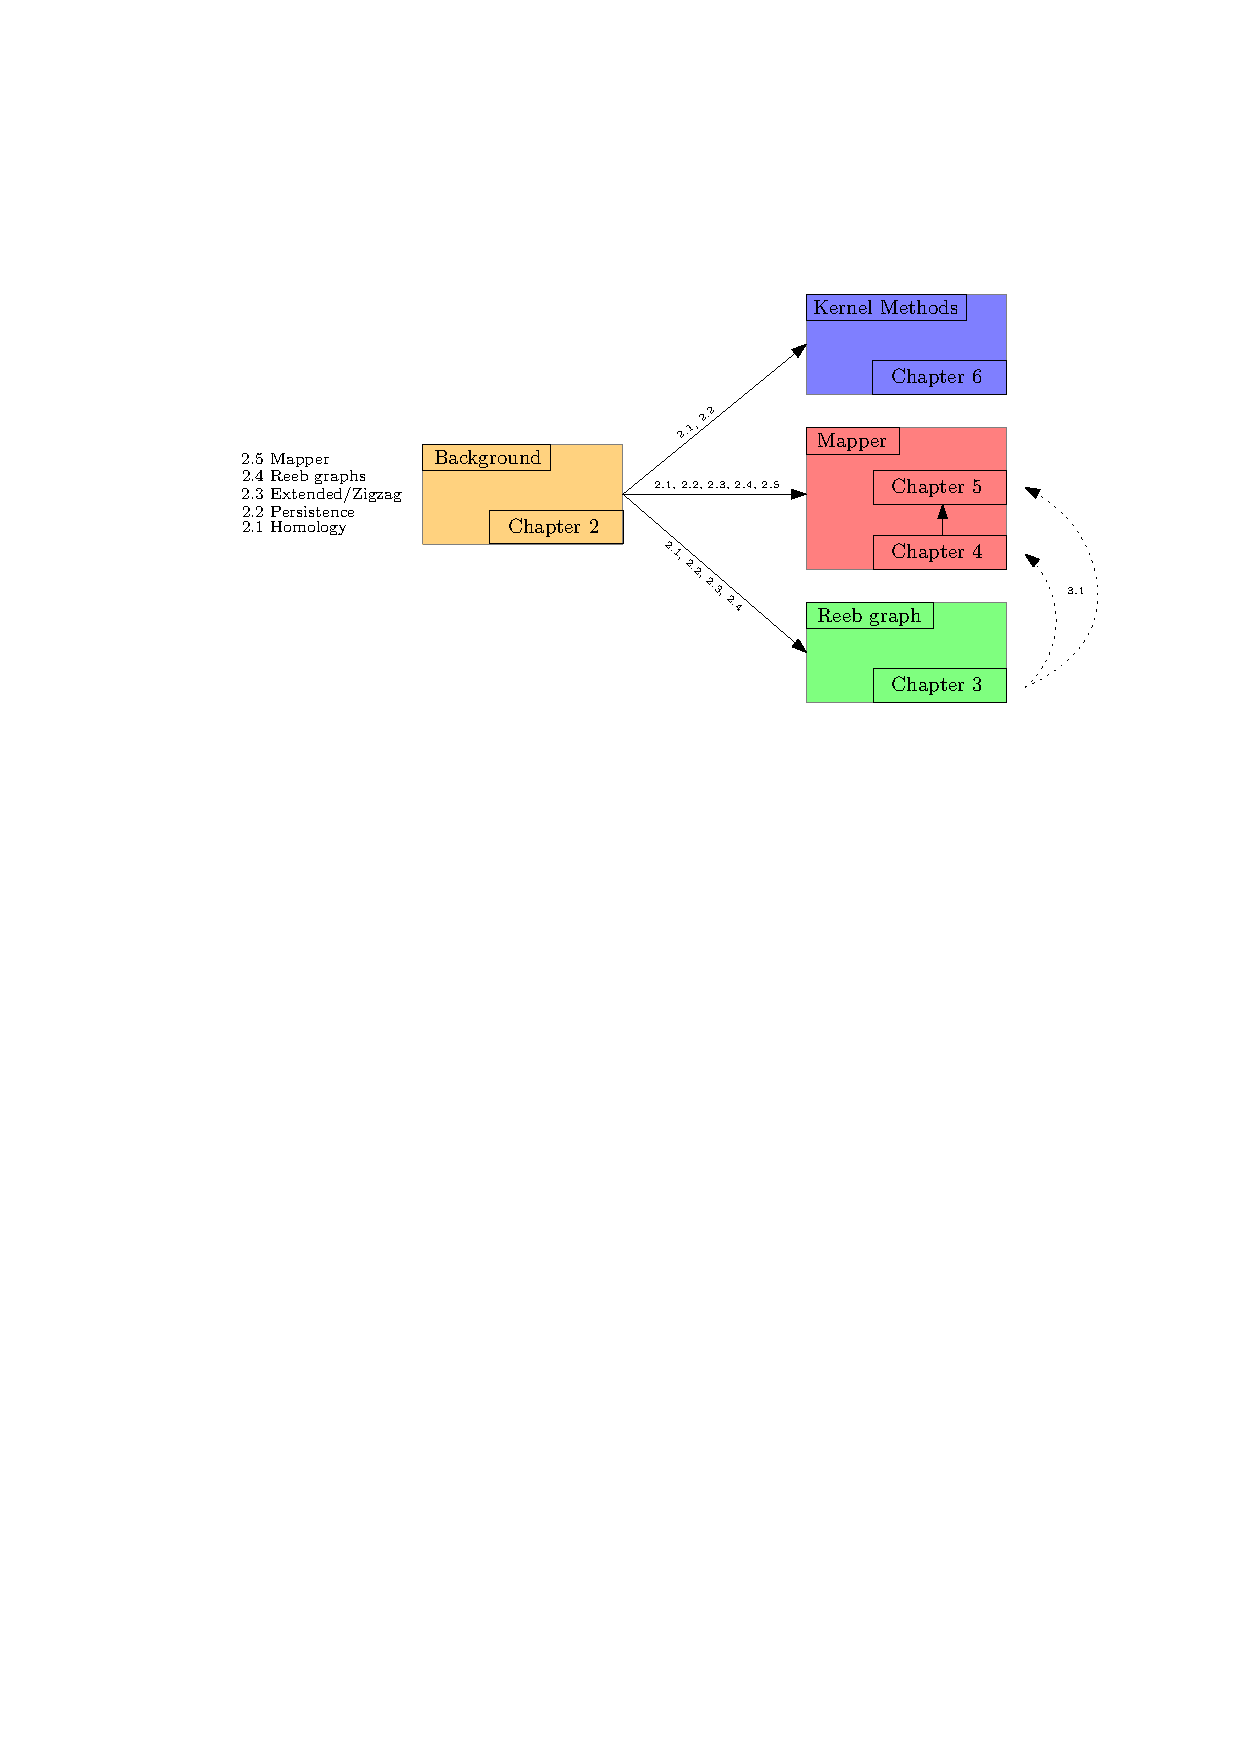
\includegraphics[width=0.95\textwidth]{figures/ThesisPlan}
\caption[Plan de la th\`ese]{\label{fig:these} Les fl\`eches indiquent des d\'ependances entre chapitres, 
et les fl\`eches en pointill\'es indiquent des d\'ependances partielles, c'est-\`a-dire que seule une petite
et non essentielle partie du chapitre d\'epend de l'autre. %Nous indiquons aussi les sections du 
%Chapitre~\ref{chap:backgroundHomologyPersistence} qui sont n\'ecessaires pour chaque partie.
}


%and dotted arrows indicate partial dependence, meaning 
%that only a small, skippable part of the chapter depends on the other. We also point out the background sections of 
%Chapter~\ref{chap:backgroundHomologyPersistence} which are required for each part.}
\end{figure}


%Hence, the reader which is unfamiliar  
%In Chapter~\ref{chap:MapperStability}, we provide links between Mapper and Reeb graphs in the case of non discrete topological spaces.
%We also define a distance between Mapper from the one between Reeb graphs introduced in the previous chapter. We also show a stability theorem 
%for Mappers equipped with this distance.
%Chapter~\ref{chap:MapperStatistic} is a direct continuation of chapter~\ref{chap:MapperStability}.
%\end{itemize}



